\section{RESULTADOS E DISCUSSÃO}

Neste capítulo, apresentam-se os resultados compostos por 315 simulações de Dinâmica Molecular, estruturadas de forma progressiva. A investigação parte de fosfolipídios puros e em misturas binárias frente a diferentes gradientes de hidratação compreendendo 105 simulações divididas em 35 réplicas cada, entre os regimes de 15, 27 e 45 moléculas de água por lipídio (W/L). Em seguida, a matriz lipídica é submetida à adição do colesterol em dois cenários distintos. No primeiro, sob hidratação de 40 W/L, executaram-se 105 simulações testando saturações de 0\%, 3\% e 30\% de colesterol. No segundo cenário, incorporou-se íons através da adição de NaCl, totalizando mais 105 simulações com proporções de 0\%, 4\% e 40\% de esterol. Por fim, mostram-se  os eixos energéticos fundamentais que governam e justificam as transformações macroscópicas observadas nos domínios estudados.

A integridade estrutural e a fase termodinâmica das bicamadas lipídicas são ditadas primariamente pelo balanço de forças laterais, expresso macroscopicamente pela área por lipídio ($A_L$). Para validar a influência do solvente na termodinâmica da bicamada, avaliou-se inicialmente o impacto de diferentes gradientes hídricos no sistema de DPPC (Figura \ref{fig:comparativo_hidratacao}). Os dados mostram que a redução da hidratação para níveis restritos (15 W/L) promove uma compressão lateral, induzindo uma transição de fase facilitada. Nota-se a convergência das curvas de expansão térmica entre os regimes de 40W/L e 45 W/L, provando que a membrana atinge o seu limite de dilatação induzida por solvente. Esta métrica estabelece 40W/L como hidratação ideal para as simulações, garantindo solvatação adequada sem os custos computacionais de simulações com mais partículas.

% --- Figura 4.1: Comparativo de Hidratação ---
\begin{figure}[htpb]
    \centering
    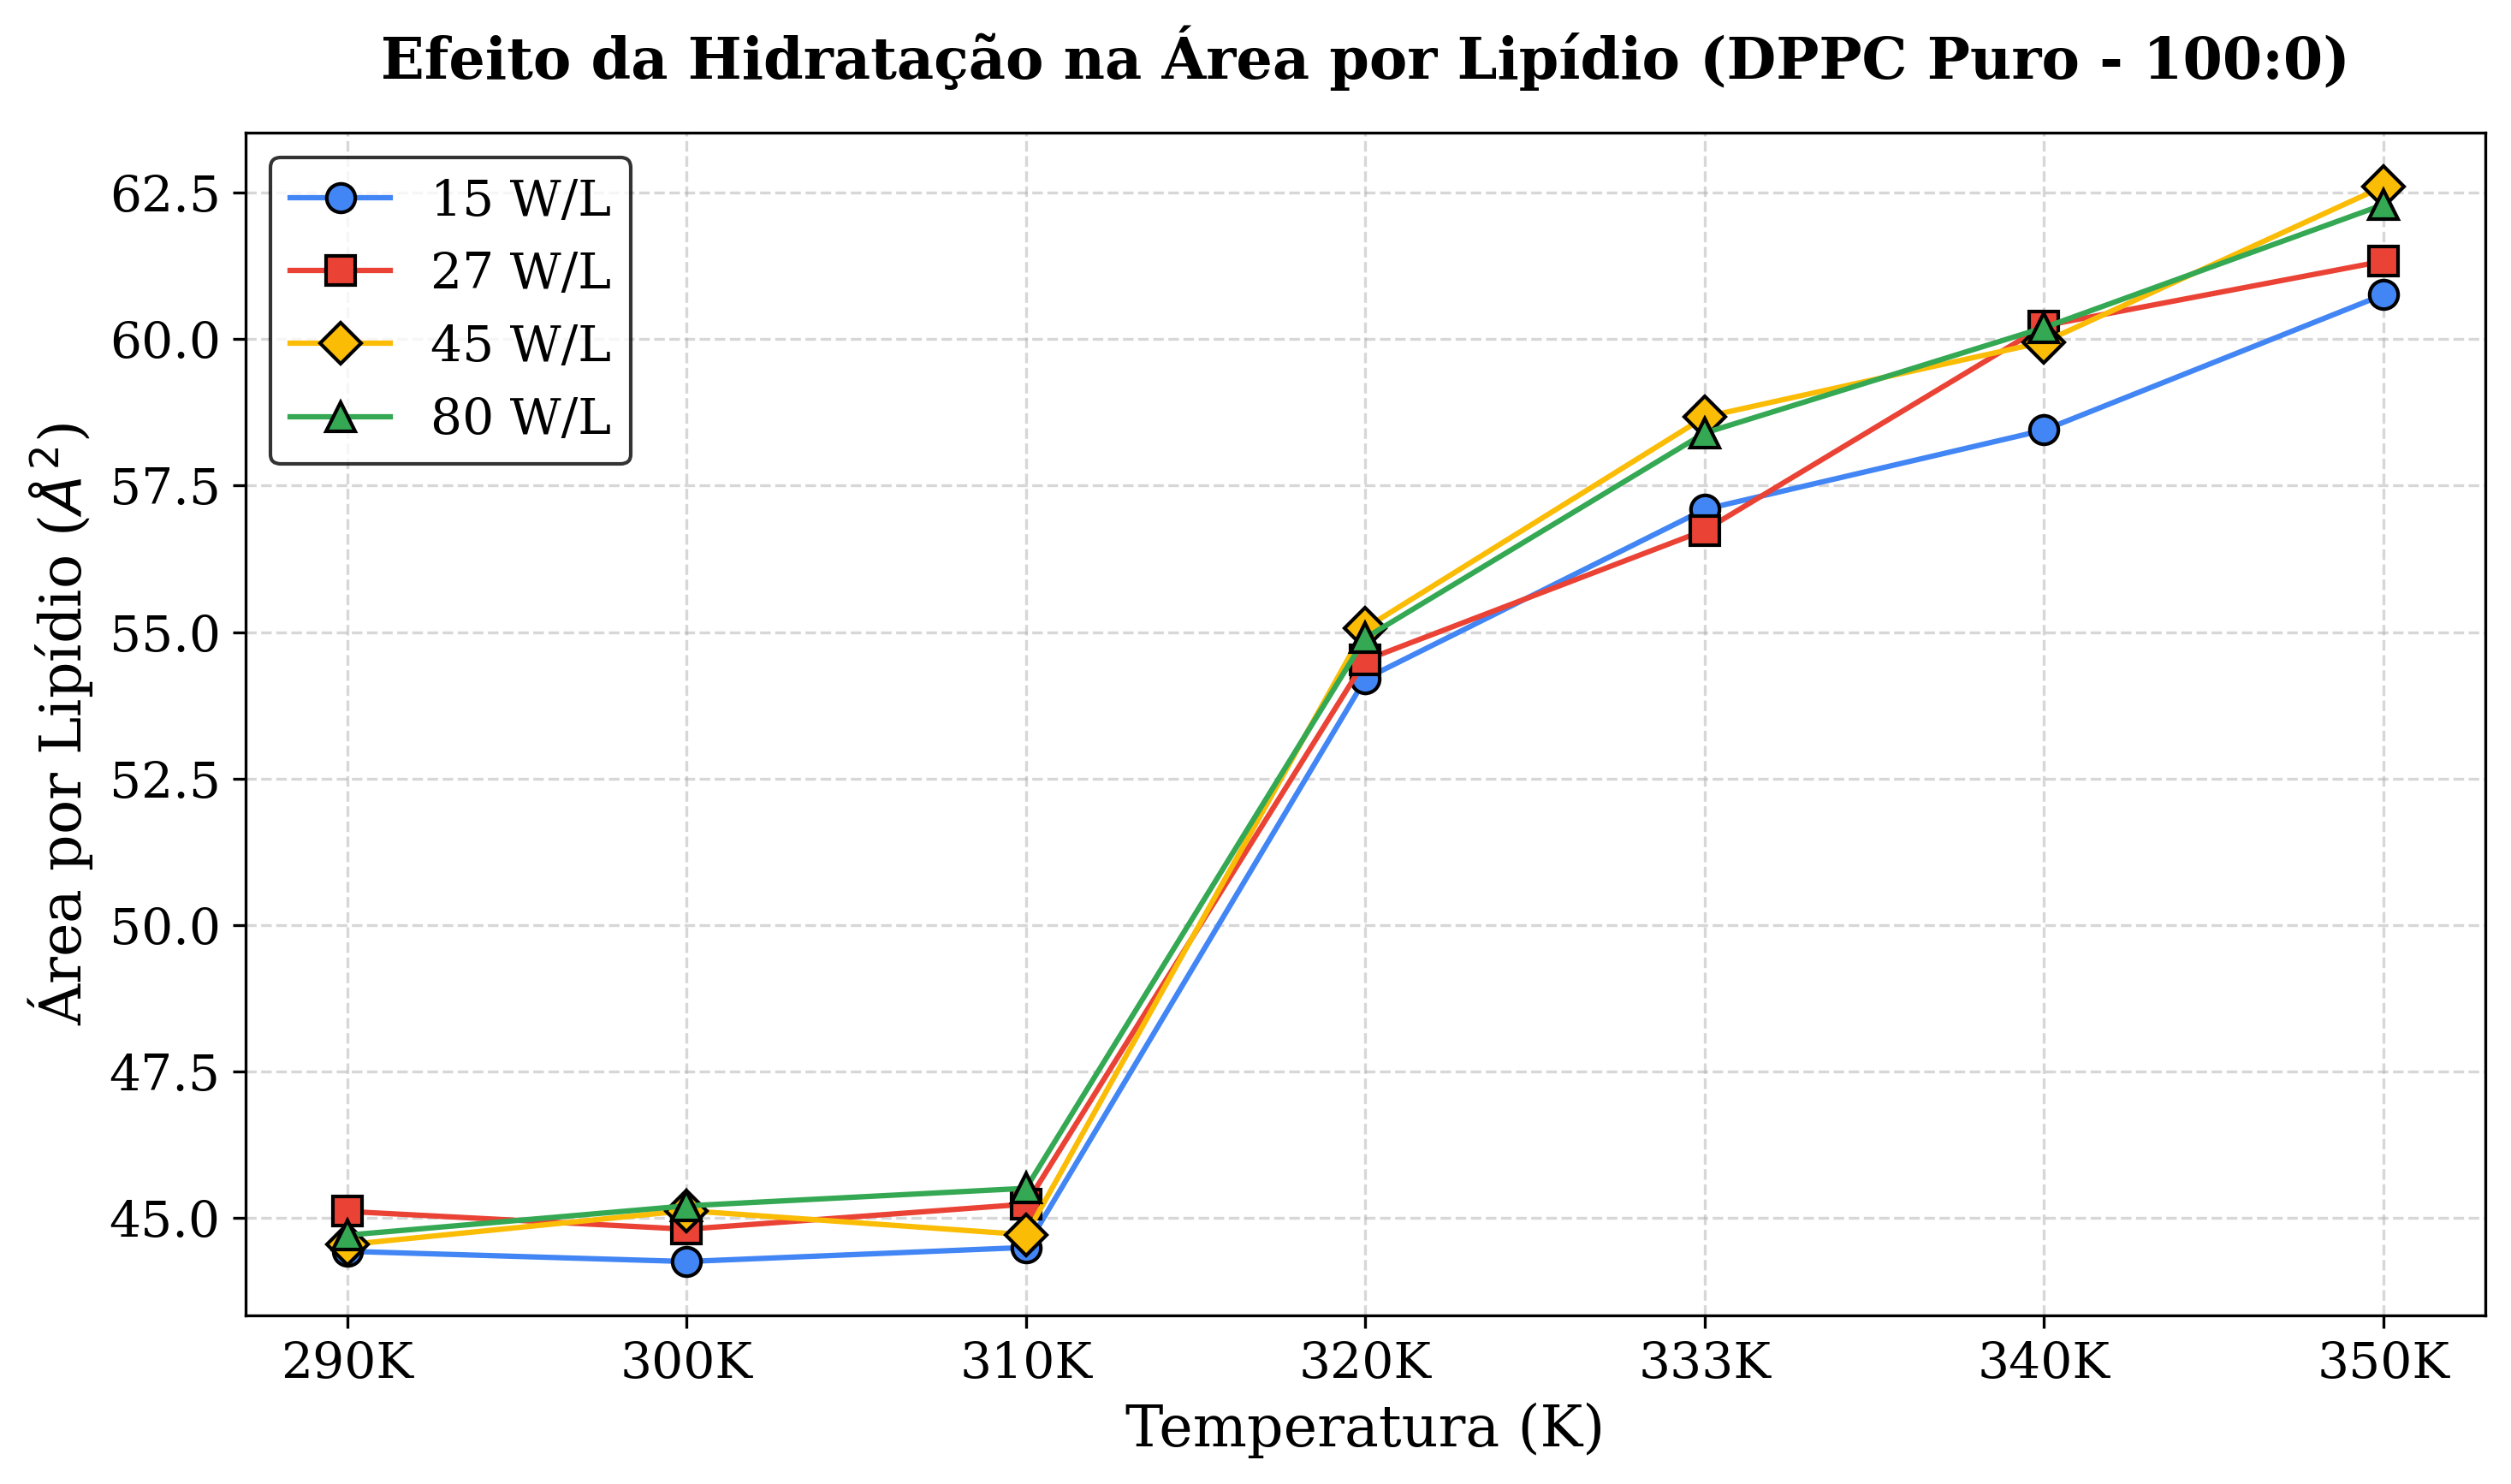
\includegraphics[width=\textwidth]{imagens/figura_4_1_google.png}
    \caption{Efeito do gradiente de hidratação na expansão térmica lateral do DPPC puro (100:0). A convergência entre os regimes de 40 W/L e 45 W/L estabelece o limite de dilatação induzida por solvente para o modelo Martini 3.}
    \label{fig:comparativo_hidratacao}
\end{figure}

A Figura \ref{fig:mosaico_4_2} reforça este panorama ao ilustrar a dinâmica de transição termotrópica para os lipídios de DPPC e DSPC puros, evidenciando os primeiros sinais de retenção cinética estrutural em regimes de média e alta hidratação. Contudo, a modelagem \textit{coarse-grained} (CG) baseada no campo de força Martini 3 envolve compromissos termodinâmicos. Para garantir a reprodução do comportamento cooperativo em misturas, o modelo impõe uma compactação artificial que subestima ligeiramente a $A_L$ na fase gel ($L_{\beta}$) e superestima a temperatura da transição principal ($T_m$) em aproximadamente 5 a 10 K \cite{pedersen2024}. 

% --- Figura 4.2: Mosaico DPPC vs DSPC ---
\begin{figure}[htpb]
    \centering
    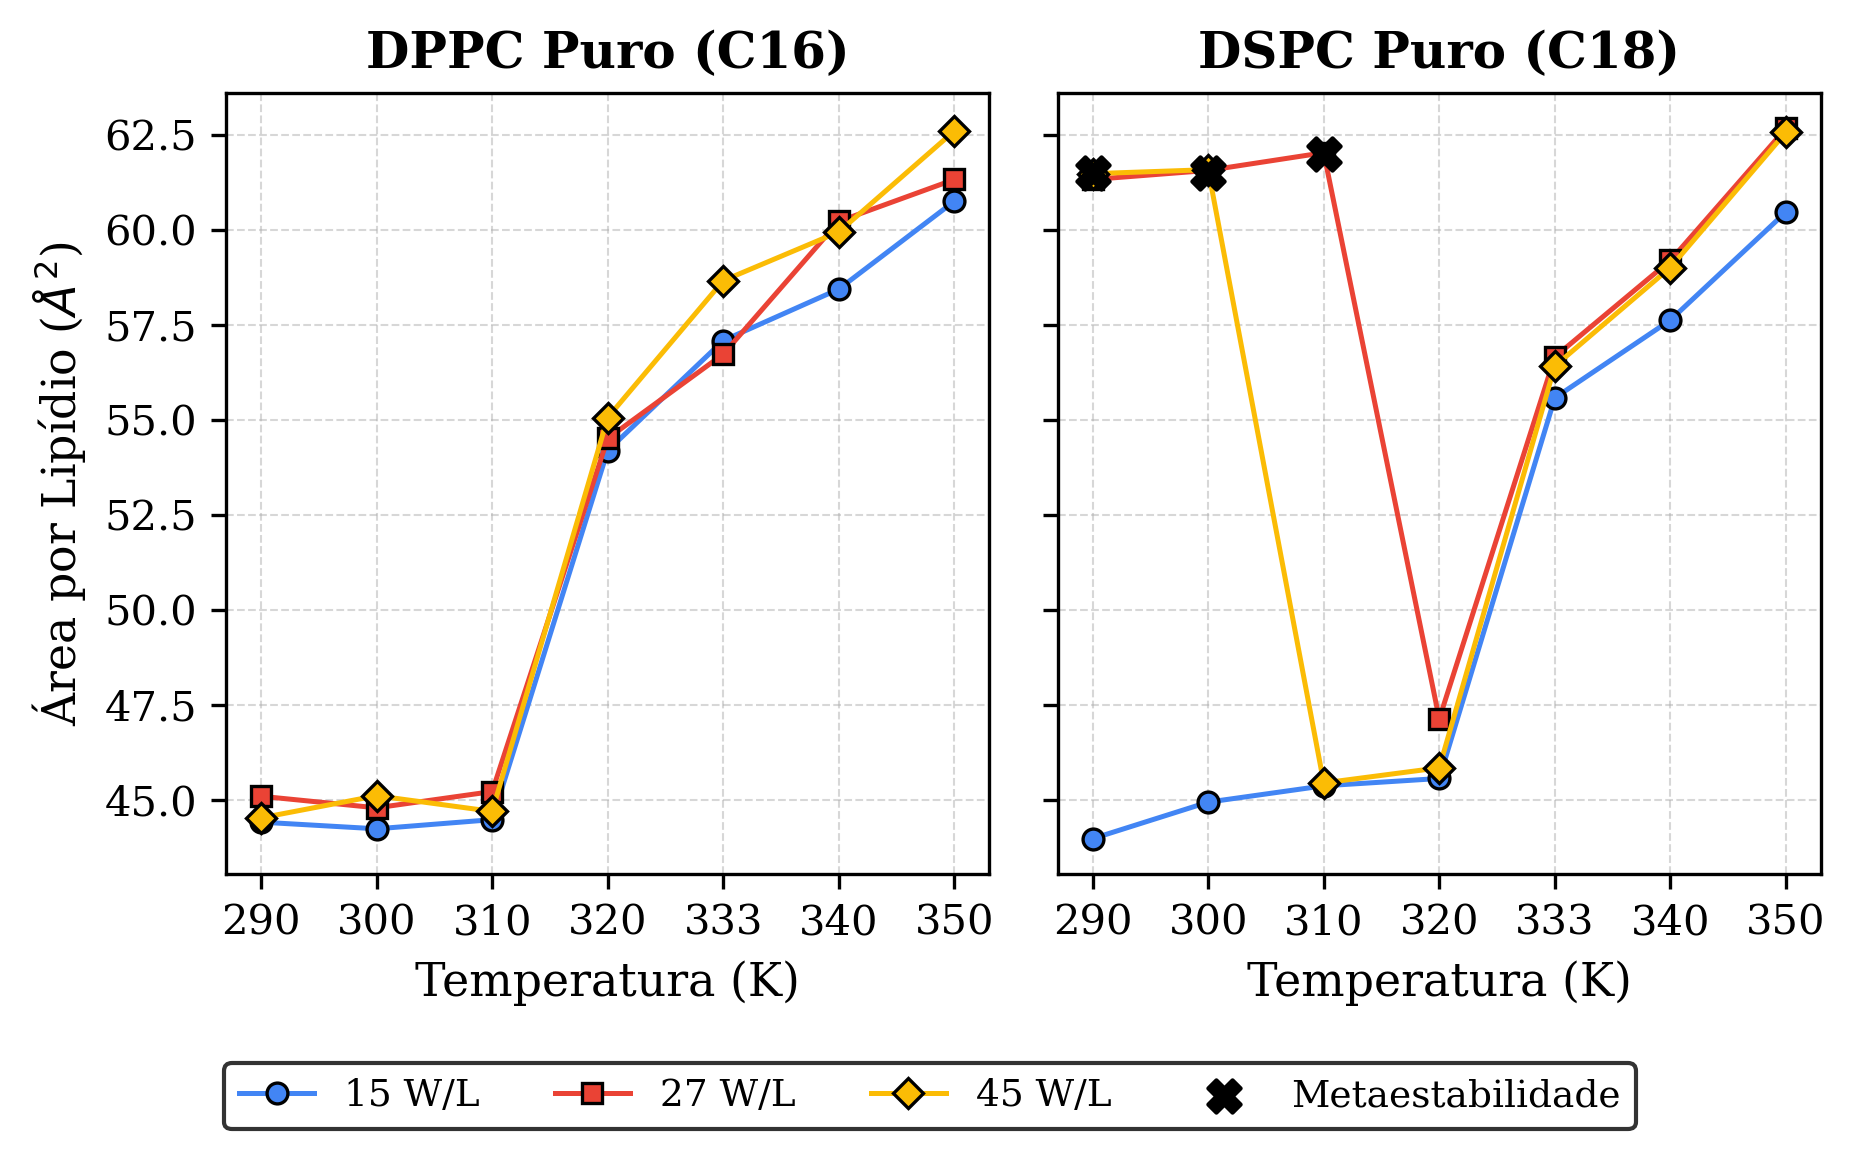
\includegraphics[width=\textwidth]{imagens/mosaico_figura_4_2.png}
    \caption{Influência da hidratação na transição termotrópica dos lipídios puros. À esquerda, a expansão do DPPC ($C_{16}$); à direita, a retenção do DSPC ($C_{18}$), evidenciando a barreira de um estado metaestável sob média e alta hidratação.}
    \label{fig:mosaico_4_2}
\end{figure}

Devido a estes desvios térmicos intrínsecos, uma comparação isotérmica direta entre as simulações e os dados experimentais seria incompatível entre os estados físicos da membrana. Para avaliar o deslocamento da temperatura de transição ($T_m$) e a metaestabilidade provocada pelo modelo Martini 3, a Tabela \ref{tab:comparativo_area} compara os estados experimentais de referência com os simulados para hidratação de 45W\_L.

\begin{table}[htpb]
    \centering
    \caption{\label{tab:comparativo_area} Comparativo da Área por Lipídio ($A_L$) em função da temperatura, evidenciando o deslocamento da transição de fase no modelo Martini 3 (sistema 45W\_L).}
    \renewcommand{\arraystretch}{1.2}
    \resizebox{\textwidth}{!}{%
    \begin{tabular}{llcccl}
        \toprule
        \multirow{2}{*}{\textbf{Lipídio}} & \multicolumn{2}{c}{\textbf{Referência Experimental \cite{kucerka2011}}} & \multicolumn{3}{c}{\textbf{Simulação Martini 3 (Este Trabalho)}} \\
        \cmidrule(lr){2-3} \cmidrule(lr){4-6}
         & \textbf{Fase a Temp. (K)} & \textbf{$A_L$ (\AA$^2$)} & \textbf{Temp. (K)} & \textbf{$A_L$ (\AA$^2$)} & \textbf{Fase Observada} \\
        \midrule
        \multirow{7}{*}{\textbf{DPPC}} & \multirow{3}{*}{Gel ($L_{\beta}$)} & \multirow{3}{*}{--}
         & 290 & $\sim 45,0$ & Gel ($L_{\beta}$) \\
         & & & 300 & $\sim 44,8$ & Gel ($L_{\beta}$) \\
         & & & 310 & $\sim 45,0$ & Gel ($L_{\beta}$) \\
        \cmidrule(lr){2-6}
         & \multirow{2}{*}{Fluida ($L_{\alpha}$) a 323} & \multirow{2}{*}{$63,1 \pm 1,3$} & 320 & $\sim 55,0$ & Transição de Fase \\
         & & & 333 & $\sim 58,6$ & Fluida ($L_{\alpha}$) \\
        \cmidrule(lr){2-6}
         & \multirow{2}{*}{Fluida ($L_{\alpha}$) a 333} & \multirow{2}{*}{$65,0 \pm 1,3$}
         & 340 & $\sim 60,0$ & Fluida ($L_{\alpha}$) \\
         & & & 350 & $\sim 62,6$ & Fluida ($L_{\alpha}$) \\
        \midrule
        \multirow{7}{*}{\textbf{DSPC}} & \multirow{4}{*}{Gel ($L_{\beta}$)} & \multirow{4}{*}{--}
         & 290 & $\sim 61,5$ & Metaestável \\
         & & & 300 & $\sim 61,5$ & Metaestável \\
         & & & 310 & $\sim 45,5$ & Gel ($L_{\beta}$) \\
         & & & 320 & $\sim 45,8$ & Gel ($L_{\beta}$) \\
        \cmidrule(lr){2-6}
         & \textit{Transição} ($T_m \approx 328$) & \textit{--} & 333 & $\sim 56,5$ & Transição de Fase \\
        \cmidrule(lr){2-6}
         & \multirow{2}{*}{Fluida ($L_{\alpha}$) a 338} & \multirow{2}{*}{$63,8 \pm 1,3$}
         & 340 & $\sim 59,0$ & Fluida ($L_{\alpha}$) \\
         & & & 350 & $\sim 62,6$ & Fluida ($L_{\alpha}$) \\
        \bottomrule
    \end{tabular}%
    }
\end{table}

Na fase fluida ($L_{\alpha}$), as simulações a 350 K convergem para um $A_L \approx 62,6$ \AA$^2$ tanto para o DPPC quanto para o DSPC. Estes valores encontram-se em concordância com os perfis de espalhamento de raios-X e nêutrons reportados pela literatura, que aferem áreas de 65,0 \AA$^2$ para o DPPC e 63,8 \AA$^2$ para o DSPC a 333 K \cite{kucerka2011}. 
O deslocamento térmico torna-se mais evidente ao observar que o DPPC simulado necessita atingir 350 K para igualar a dilatação que o lipídio \textit{in vivo} atinge a 323 K. No regime de gel ($L_{\beta}$), as simulações estabilizam em torno de 45,0 \AA$^2$, refletindo a compactação artificial do campo de força e justificando a ampla janela de transição térmica.

Este alargamento da transição térmica e a exigência de superaquecimento (necessitando atingir 350 K para a estabilização da fase fluida) contrastam com a característica das transições observadas \textit{in vitro}. Contudo, tal comportamento não indica ausência de equilíbrio, mas reflete fenômenos intrínsecos à simulação nesta metodologia. Embora suprimir os graus de liberdade, atuando como facilitador cinético para o efeito de avalanche termodinâmica, é exigido uma maior injeção de energia térmica para desestabilizar a rede lamelar. Em segundo lugar, a mecânica estatística estabelece que singularidades perfeitas de transição só emergem no limite termodinâmico ($N \to \infty$). Em sistemas sob nanoconfinamento, as flutuações de borda impõem o Efeito de Tamanho Finito (\textit{Finite-Size Effect \cite{hal_finitesize}}\cite{piskulich2022} ), que invariavelmente borra a curva de transição. Por fim, as extrações de energia foram parametrizadas para a totalidade da caixa, englobando as moléculas do solvente, que atua como reservatório termodinâmico, cuja expansão térmica  distorce o sinal macroscópico da fusão hidrofóbica interna.

A termodinâmica do sistema de DSPC puro no modelo utilizado, evidenciada pela série temporal da Figura \ref{fig:estabilidade}, em 290 K e 300 K, falha em nuclear espontaneamente, permanecendo retida num estado metaestável. Consequência do limite de resolução do mapeamento CG, que agrupa múltiplos átomos em esferas interativas, suprimindo as flutuações individuais. A divergência de nucleação entre o DPPC e o DSPC valida a sensibilidade do modelo. Para discriminar caudas lipídicas com diferença de dois carbonos, o DPPC utiliza contas de menor raio (\textit{small beads}), diminuindo o volume colisional. Em contrapartida, as caudas do DSPC são mapeadas com contas regulares \cite{pedersen2024}. O maior raio aumenta a fricção, fazendo com que as flutuações térmicas ($k_B T$) sejam insuficientes para superar a penalidade entálpica, mantendo a membrana no mesmo estado..

% --- Figura 4.4: Estabilidade / Série Temporal ---
\begin{figure}[htpb]
    \centering
    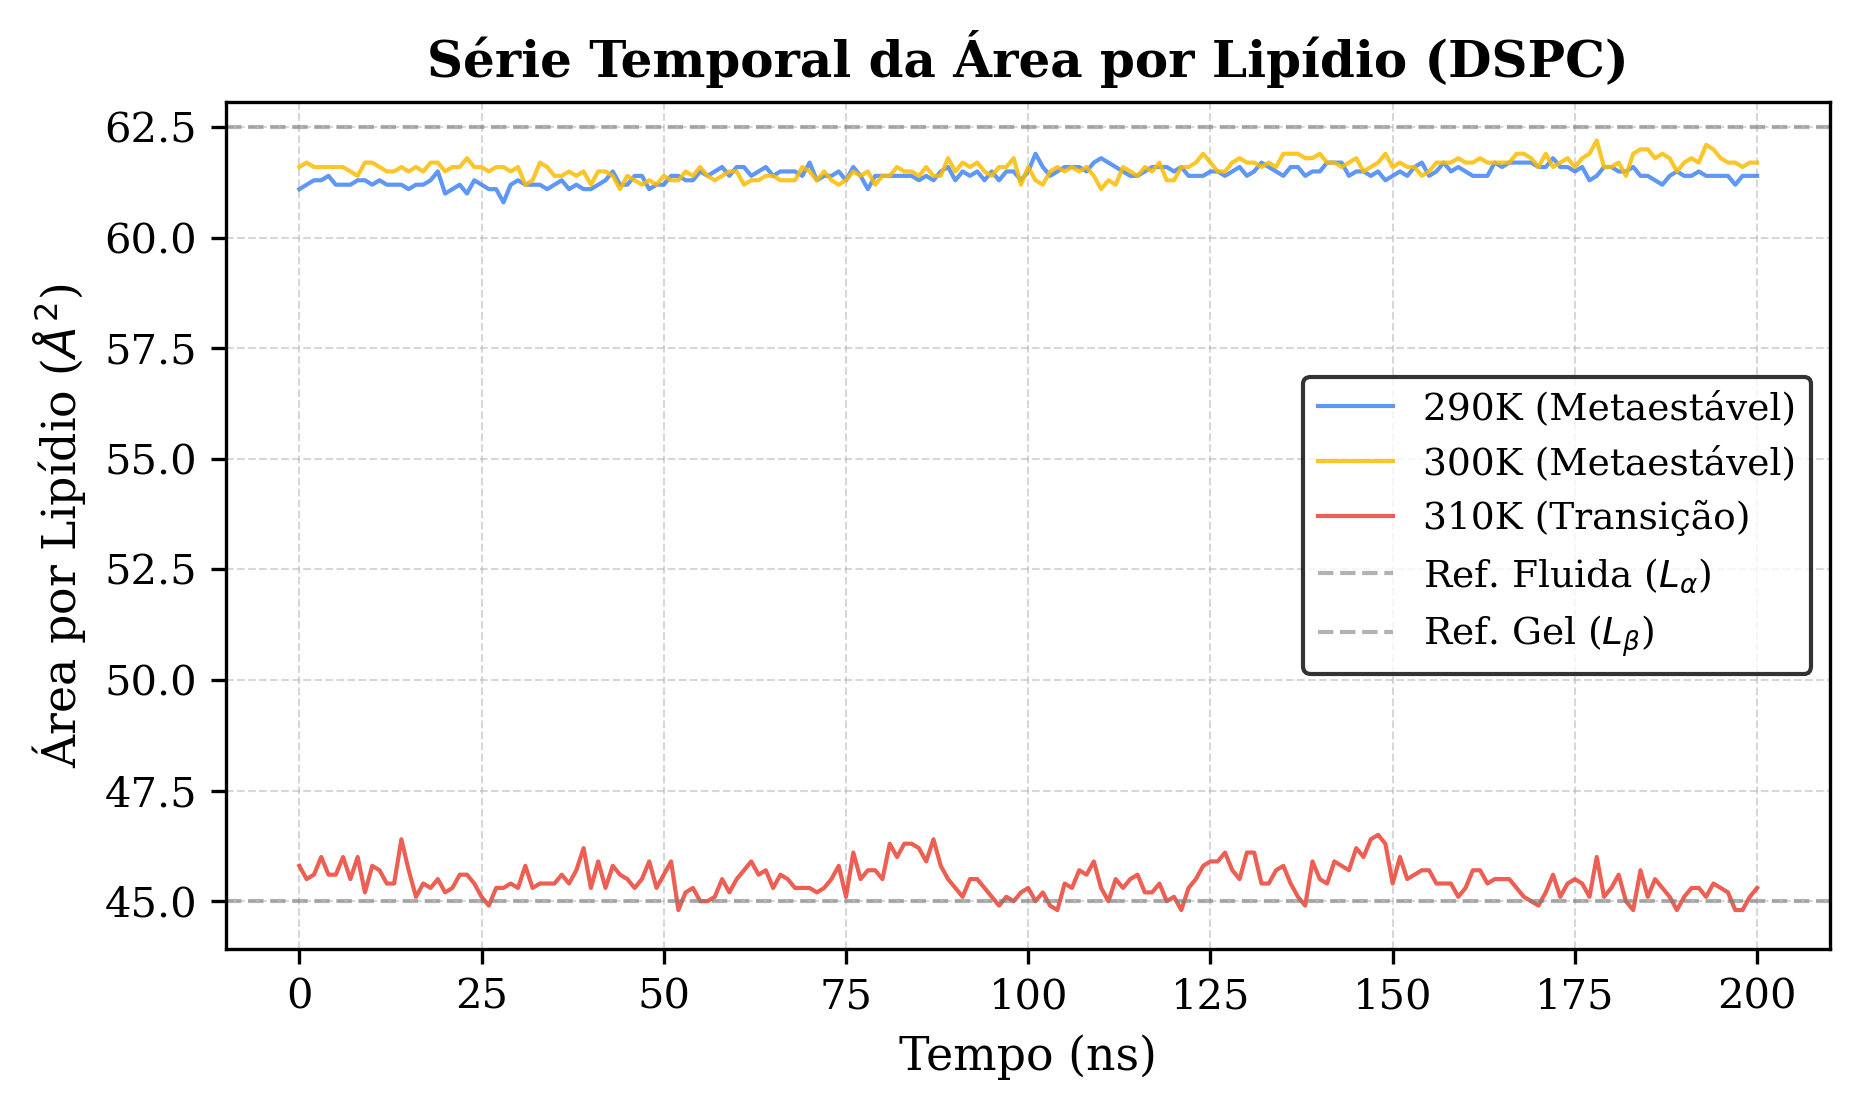
\includegraphics[width=\textwidth]{imagens/analise_estabilidade_DSPC_completa.png}
    \caption{Série temporal evidenciando a barreira de nucleação no DSPC puro (45W\_L). As trajetórias a 290 K e 300 K falham em transicionar espontaneamente para a fase gel ($L_{\beta}$) ao longo de 200 ns de simulação.}
    \label{fig:estabilidade}
\end{figure}

A restrição hídrica altera fundamentalmente a energia livre. No sistema de baixa hidratação (15W\_L, Figura \ref{fig:apl_15w}), a diminuição do volume e da blindagem dielétrica elimina a barreira de repulsão hídrica. Isso suprime a metaestabilidade, induzindo uma transição de fase para o DSPC. O regime intermediário (27W\_L, Figura \ref{fig:apl_27w}) atua como uma transição mecânica, onde a membrana ainda inicia retida em metaestabilidade, mas exibe uma cristalização tardia a 320 K.

% --- Figura 4.5: APL Baixa Hidratação (15W\_L) ---
\begin{figure}[htpb]
    \centering
    \includegraphics[width=\textwidth]{imagens/grafico_APL_15W\_L.png}
    \caption{Área por lipídio sob restrição hídrica (15W\_L). A diminuição da blindagem dielétrica e do volume livre de solvente suprime os estados metaestáveis, induzindo uma transição de fase.}
    \label{fig:apl_15w}
\end{figure}

% --- Figura 4.6: APL Média Hidratação (27W\_L) ---
\begin{figure}[htpb]
    \centering
    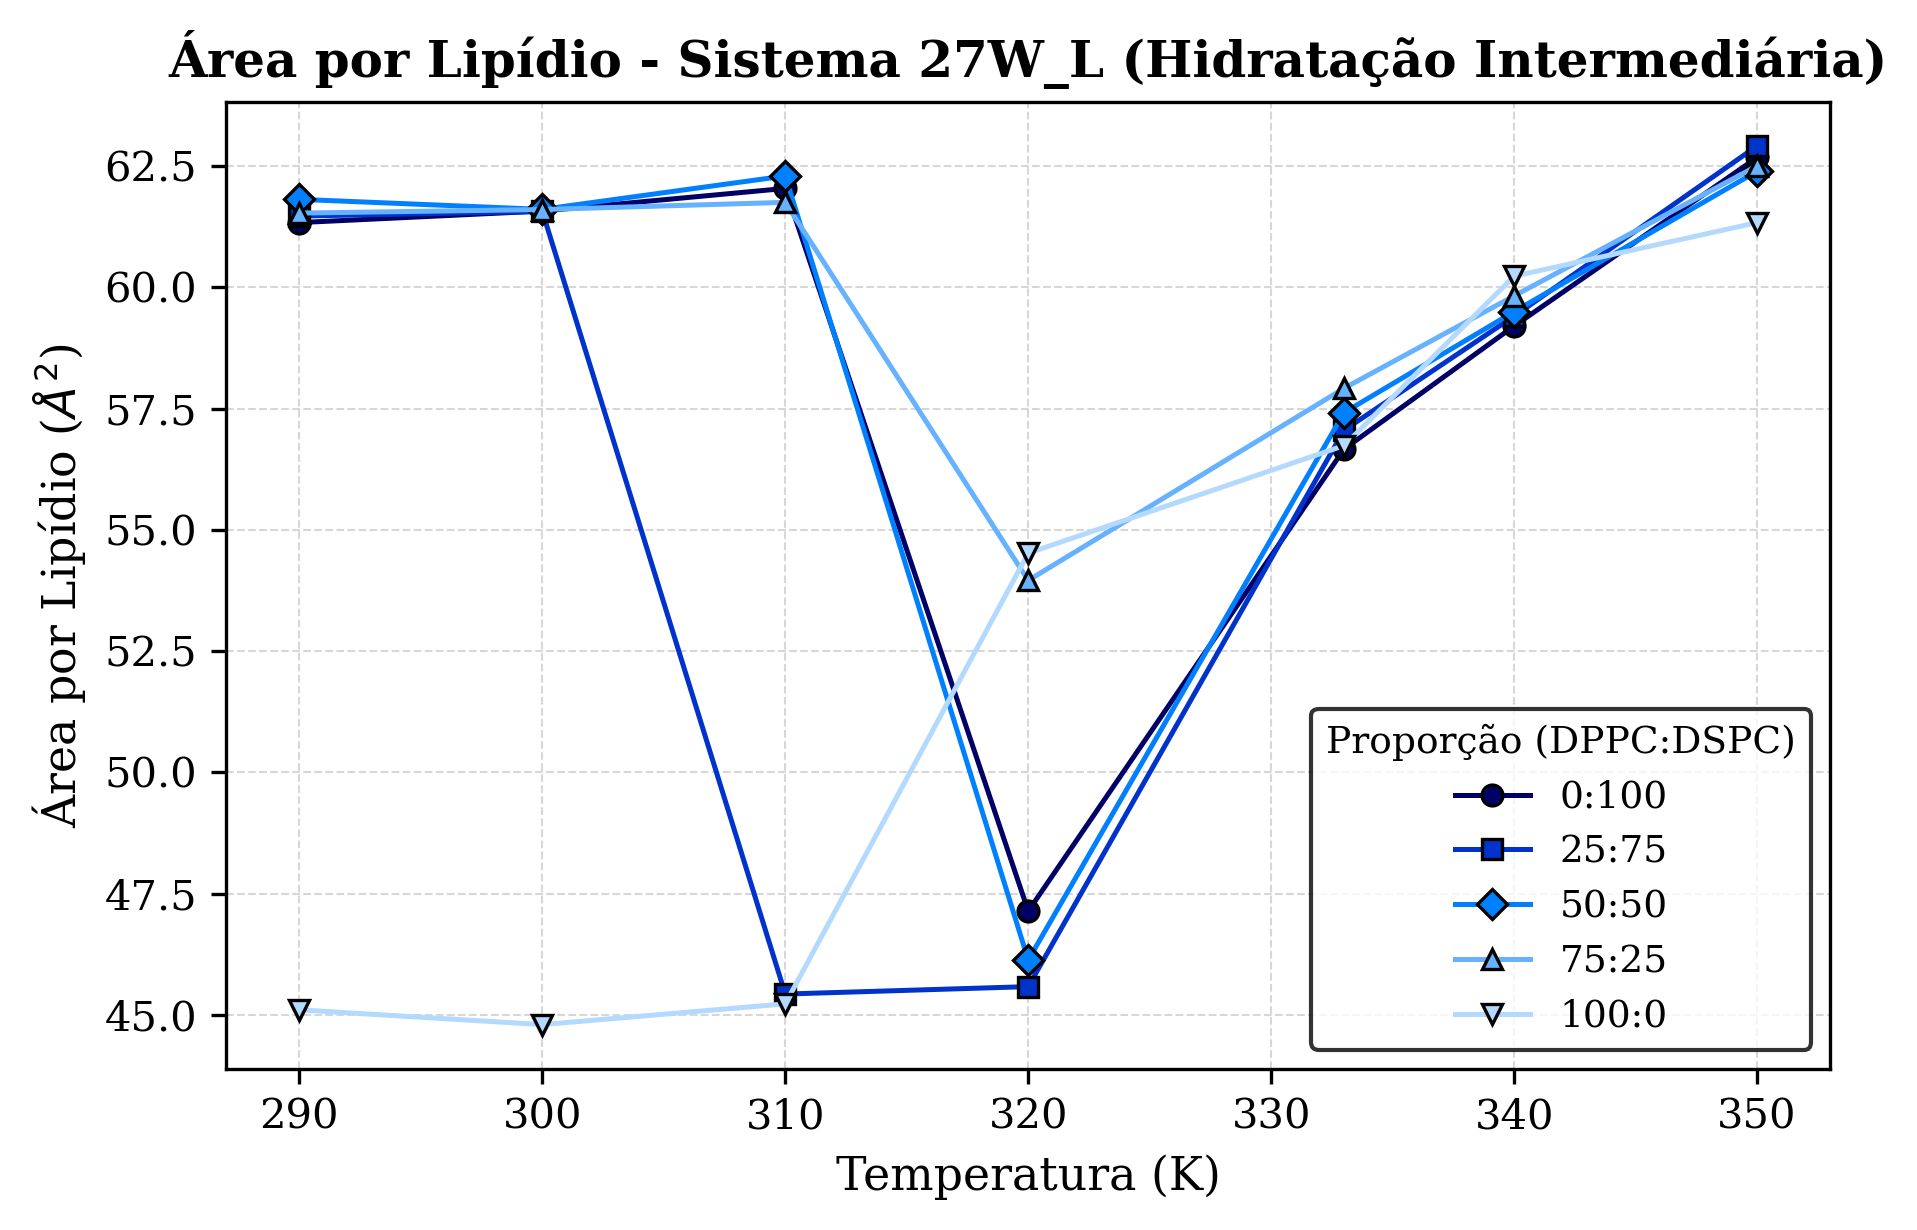
\includegraphics[width=\textwidth]{imagens/grafico_APL_27W_L.png}
    \caption{Área por lipídio sob hidratação intermediária (27W\_L). O sistema atua como um regime de transição, onde a matriz de DSPC inicia na fase fluida a 290 K, mas cede a uma cristalização a 320 K.}
    \label{fig:apl_27w}
\end{figure}

A heterogeneidade molecular atua como um contorno para esta  barreira termodinâmica. A Figura \ref{fig:mosaico_misturas} mostra este comportamento através das misturas binárias. As misturas apresentam zonas de coexistência onde a inclusão de cadeias mais curtas ($C_{16}$, DPPC) nas matrizes de DSPC atua como um facilitador, reduzindo a energia de ativação necessária para o rearranjo do empacotamento apolar e restaurando a cooperatividade da transição.

% --- Figura 4.7: Mosaico Global das Misturas ---
\begin{figure}[htpb]
    \centering
    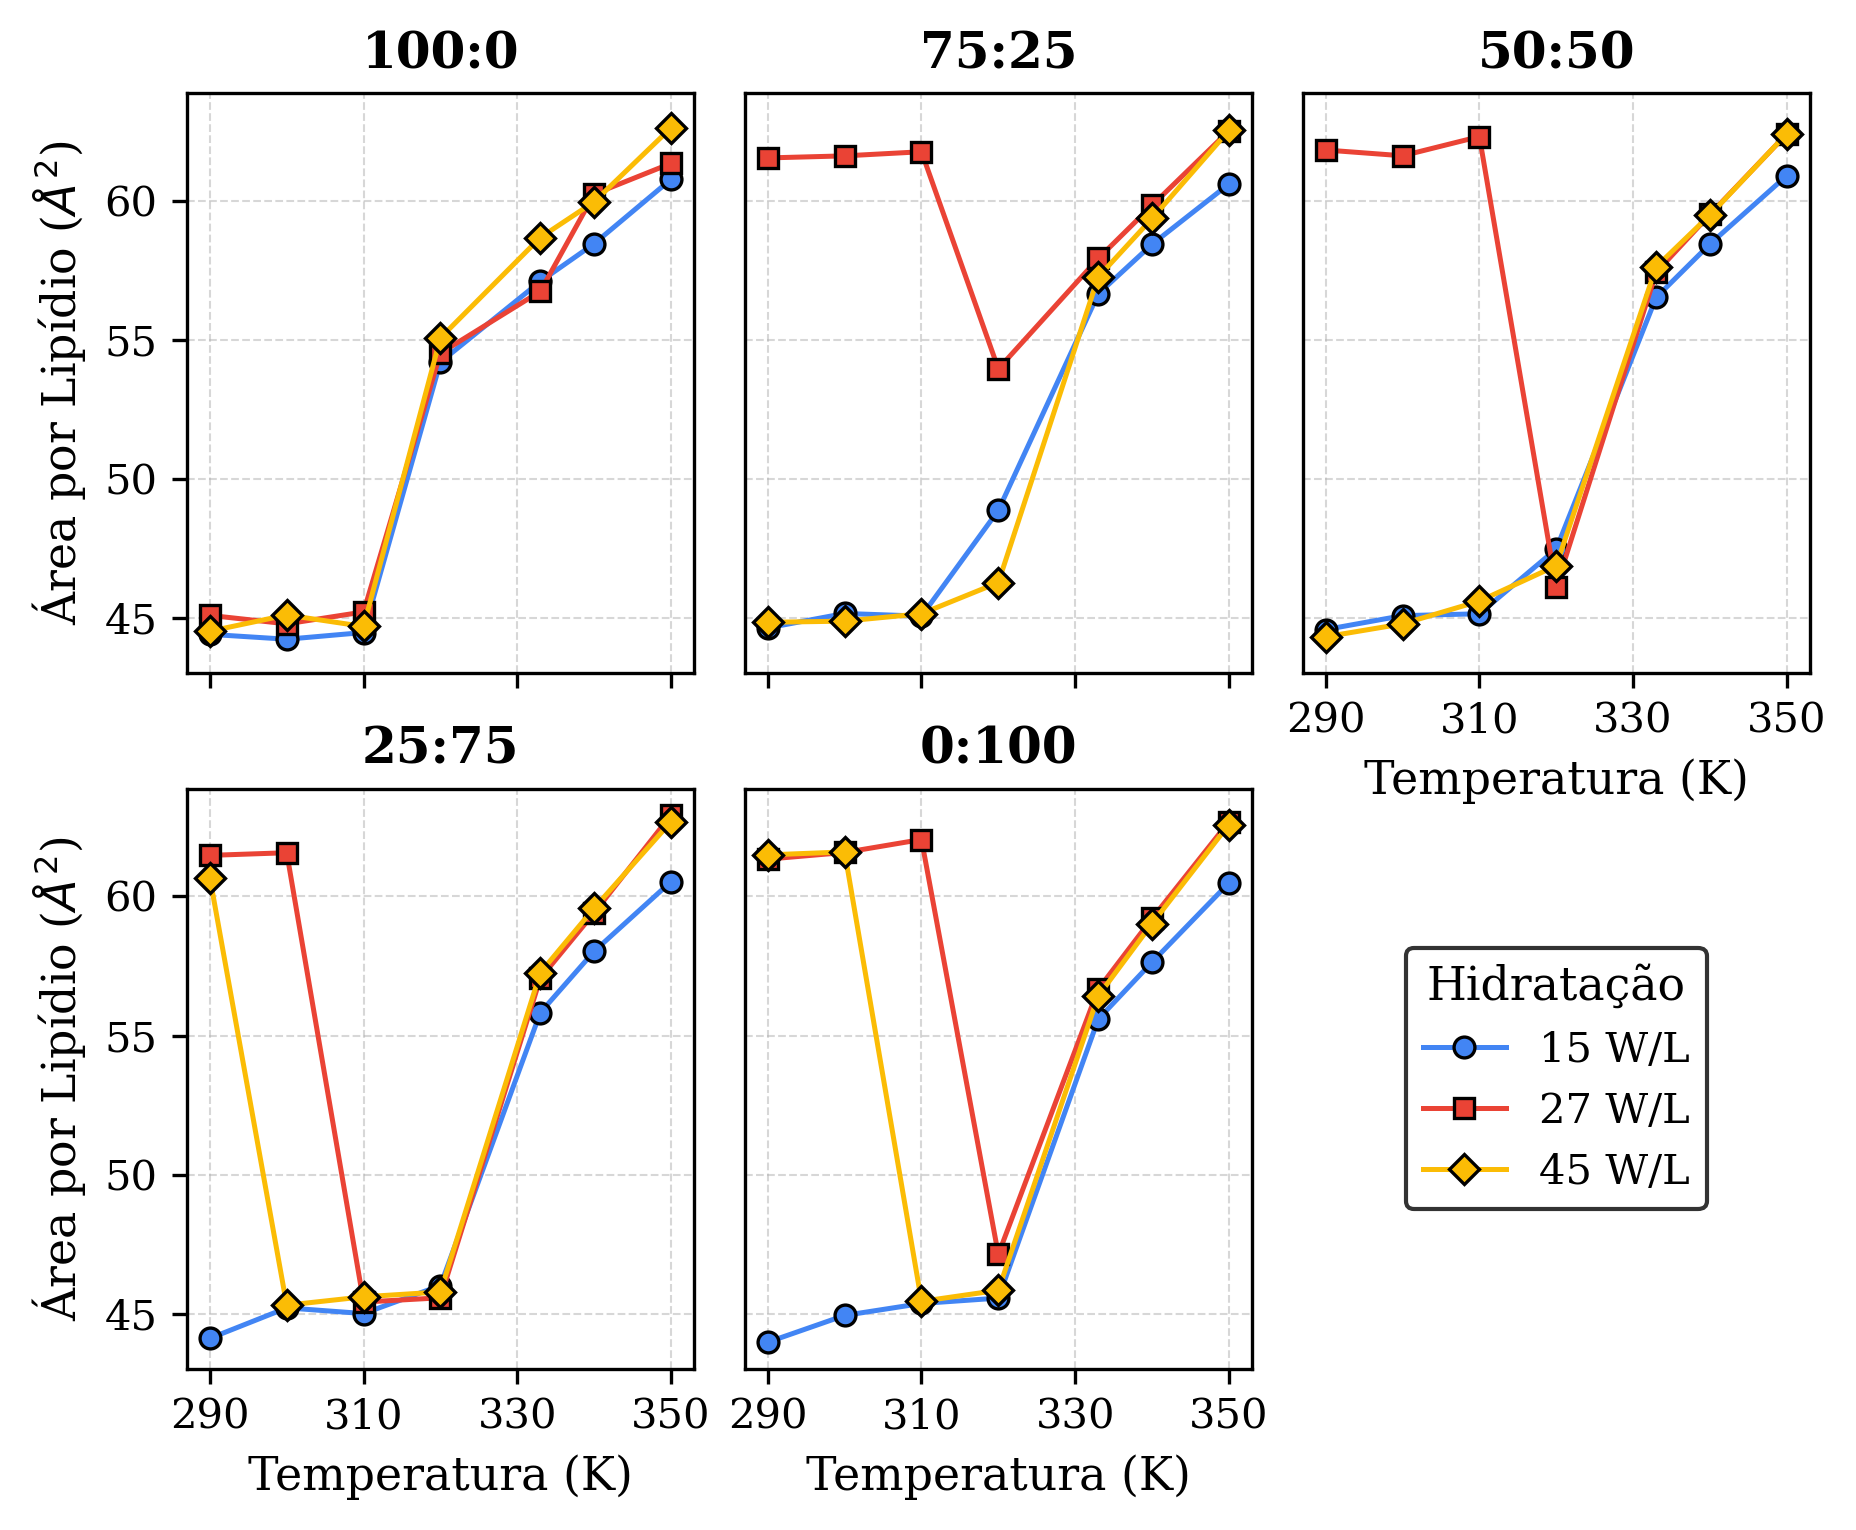
\includegraphics[width=\textwidth]{imagens/comparativo_global_misturas.png}
    \caption{Mosaico global da expansão térmica para as misturas binárias sob três diferentes regimes hídricos. Observa-se que a inclusão de DPPC ($C_{16}$) nas matrizes com DSPC atua como facilitador, restaurando a transição de fase nas hidratações mais altas.}
    \label{fig:mosaico_misturas}
\end{figure}

% --- INSIRA O SEU TEXTO ORIGINAL SOBRE A ESPESSURA (FIGURA 4.8) A PARTIR DESTE PONTO ---


\subsubsection*{Espessura da Bicamada e Efeito do Comprimento da Cadeia}

Para complementar a análise termodinâmica da área por lipídio, a espessura da membrana, distância transversal média entre os grupos polares, foi investigada em função da temperatura para o sistema de alta hidratação (45W\_L). Como ilustrado na Figura \ref{fig:espessura_45W_L}, a secção transversal da bicamada apresenta correlação inversamente proporcional à sua expansão lateral.

% --- Figura: Espessura da Membrana (A imagem que havia sumido) ---
\begin{figure}[htpb]
    \centering
    % Substitua o nome do arquivo abaixo pelo nome exato da sua imagem de espessura!
    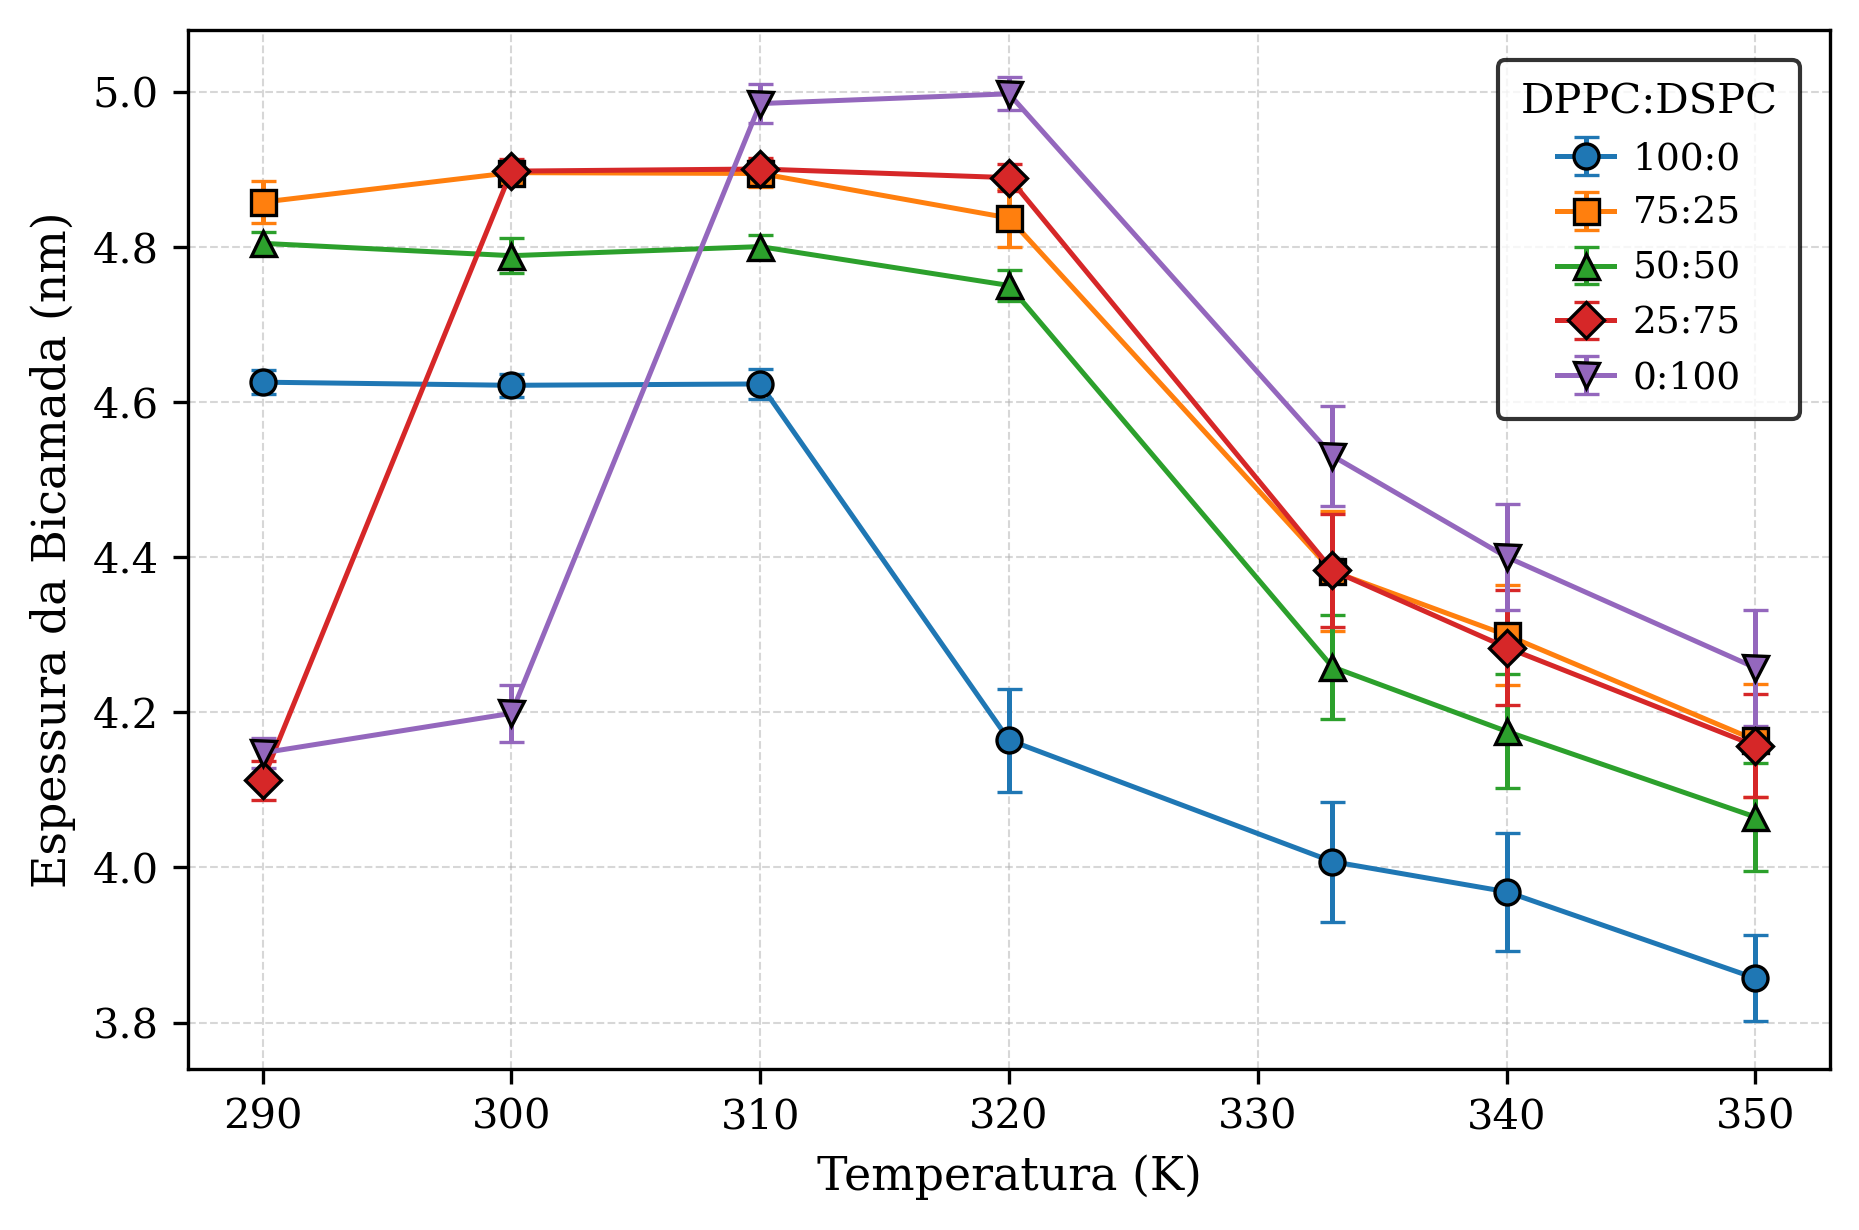
\includegraphics[width=0.85\textwidth]{imagens/grafico_espessura_45W_L.png}
    \caption{Evolução termotrópica da Espessura da Bicamada ($D_B$) sob alta hidratação (45 W/L). A expansão térmica lateral exige, por conservação de volume, a contração transversal do núcleo hidrofóbico. Nota-se que a espessura é alterada pelo comprimento das caudas ($C_{16}$ vs. $C_{18}$).}
    \label{fig:espessura_45W_L}
\end{figure}

Na fase gel ($T < 310$ K), as cadeias acílicas encontram-se altamente ordenadas e estendidas na conformação \textit{all-trans}, resultando em espessuras máximas que atingem aproximadamente $4,6$ nm para a matriz de DPPC e $5,0$ nm para o DSPC. O incremento térmico e a transição para a fase fluida ($L_\alpha$) elevam a probabilidade de isomerizações rotacionais \textit{trans-gauche}, induzindo desordem nas cadeias hidrocarbônicas \cite{kucerka2011}. Mecanicamente, esta desordem térmica exige a dilatação lateral da estrutura e a sua consequente contração transversal, evidenciada pela queda nas curvas termotrópicas.


Este comportamento e a dependência em relação ao comprimento da cadeia espelham as tendências estruturais reportadas em ensaios de espalhamento de raios-X e nêutrons \cite{kucerka2011}. Na fase fluida, a espessura total ($D_B$) é sistematicamente superior para o lipídio com mais carbono. Termodinamicamente, o incremento das interações atrativas de van der Waals nas caudas maiores atua como um contrapeso entálpico, mitigando parcialmente a diferença de espessura induzida pela desordem térmica.

Assim como observado na dinâmica de dilatação lateral, a comparação direta mascararia o deslocamento térmico inerente à modelagem. Para avaliar a precisão estrutural do mapeamento ao longo das diferentes fases físicas, a Tabela \ref{tab:comparativo_espessura} alinha a varredura térmica completa da espessura simulada com os referenciais experimentais correspondentes.

\begin{table}[htpb]
    \centering
    \caption{\label{tab:comparativo_espessura} Comparativo detalhado da evolução da Espessura da Bicamada ($D_B$) em função da temperatura, evidenciando a correlação termomecânica no modelo Martini 3 (sistema 45W\_L).}
    \label{tab:comparativo_wespessura}
    \renewcommand{\arraystretch}{1.2}
    \resizebox{\textwidth}{!}{%
    \begin{tabular}{llcccl}
        \toprule
        \multirow{2}{*}{\textbf{Lipídio}} & \multicolumn{2}{c}{\textbf{Referência Experimental \cite{kucerka2011}}} & \multicolumn{3}{c}{\textbf{Simulação Martini 3 (Este Trabalho)}} \\
        \cmidrule(lr){2-3} \cmidrule(lr){4-6}
         & \textbf{Fase a Temp. (K)} & \textbf{Espessura (nm)} & \textbf{Temp. (K)} & \textbf{Espessura (nm)} & \textbf{Fase Observada} \\
        \midrule
        \multirow{7}{*}{\textbf{DPPC}} & \multirow{3}{*}{Gel ($L_{\beta}$)} & \multirow{3}{*}{--}
         & 290 & $\sim 4,62$ & Gel ($L_{\beta}$) \\
         & & & 300 & $\sim 4,62$ & Gel ($L_{\beta}$) \\
         & & & 310 & $\sim 4,62$ & Gel ($L_{\beta}$) \\
        \cmidrule(lr){2-6}
         & \multirow{2}{*}{Fluida ($L_{\alpha}$) a 323} & \multirow{2}{*}{$3,90 \pm 0,08$} & 320 & $\sim 4,16$ & Transição de Fase \\
         & & & 333 & $\sim 4,01$ & Fluida ($L_{\alpha}$) \\
        \cmidrule(lr){2-6}
         & \multirow{2}{*}{Fluida ($L_{\alpha}$) a 333} & \multirow{2}{*}{$3,81 \pm 0,08$}
         & 340 & $\sim 3,97$ & Fluida ($L_{\alpha}$) \\
         & & & 350 & $\sim 3,85$ & Fluida ($L_{\alpha}$) \\
        \midrule
        \multirow{7}{*}{\textbf{DSPC}} & \multirow{4}{*}{Gel ($L_{\beta}$)} & \multirow{4}{*}{--}
         & 290 & $\sim 4,15$ & Metaestável \\
         & & & 300 & $\sim 4,20$ & Metaestável  \\
         & & & 310 & $\sim 4,98$ & Gel ($L_{\beta}$) \\
         & & & 320 & $\sim 5,00$ & Gel ($L_{\beta}$) \\
        \cmidrule(lr){2-6}
         & \textit{Transição} ($T_m \approx 328$) & \textit{--} & 333 & $\sim 4,53$ & Transição de Fase \\
        \cmidrule(lr){2-6}
         & \multirow{2}{*}{Fluida ($L_{\alpha}$) a 338} & \multirow{2}{*}{$4,22 \pm 0,08$}
         & 340 & $\sim 4,40$ & Fluida ($L_{\alpha}$) \\
         & & & 350 & $\sim 4,25$ & Fluida ($L_{\alpha}$) \\
        \bottomrule
    \end{tabular}%
    }
\end{table}

A análise quantitativa revela a precisão estrutural da simplificação molecular. A literatura estabelece espessuras experimentais de $3,90$ nm para o DPPC (a 323 K) e $4,22$ nm para o DSPC (a 333 K) \cite{kucerka2011}. No limite superior do regime totalmente fluido simulado (350 K), a secção transversal converge para $\sim 3,85$ nm no sistema de DPPC, enquanto o DSPC estabiliza-se em $\sim 4,25$ nm. A proximidade destes dados estruturais entre $C_{16}$ e $C_{18}$ valida a capacidade da discretização topológica em reproduzir as caracteristicas do empacotamento hidrofóbico.

Este comportamento atesta que a dependência térmica das propriedades geométricas da bicamada lipídica é reproduzida de maneira fisicamente coerente: a elevação da temperatura conduz ao incremento da Área por Lipídio e à respectiva diminuição da espessura da bicamada, o que consolida os parâmetros calibrados no modelo \cite{pedersen2025}.

Por fim, a secção transversal do DSPC, nas temperaturas em que a membrana permaneceu aprisionada em metaestabilidade (290 K e 300 K), a espessura também exibiu uma anomalia, comprovando que a presença da água de hidratação inviabilizou o estiramento vertical pleno das caudas apolares. Os dados aos 310 K, sinaliza a expulsão da água interfacial e atua como a resposta morfológica da cristalização mecânica para a fase gel ($L_{\beta}$).

\subsection{Efeito Condensador do Colesterol}

A introdução de colesterol na matriz lipídica altera fundamentalmente a termodinâmica da bicamada. Para isolar o efeito estrutural do esterol, avaliou-se inicialmente o sistema sob hidratação de 40 W/L na ausência de íons. O mosaico global da expansão térmica (Figura \ref{fig:mosaico_chol_global}) mostra o impacto de concentrações crescentes de colesterol (0\%, 3\% e 30\% em mol) sobre as misturas binárias de DPPC e DSPC.

% --- Figura 4.8: Mosaico Global do Colesterol (Sem Íons) ---
\begin{figure}[htpb]
    \centering
    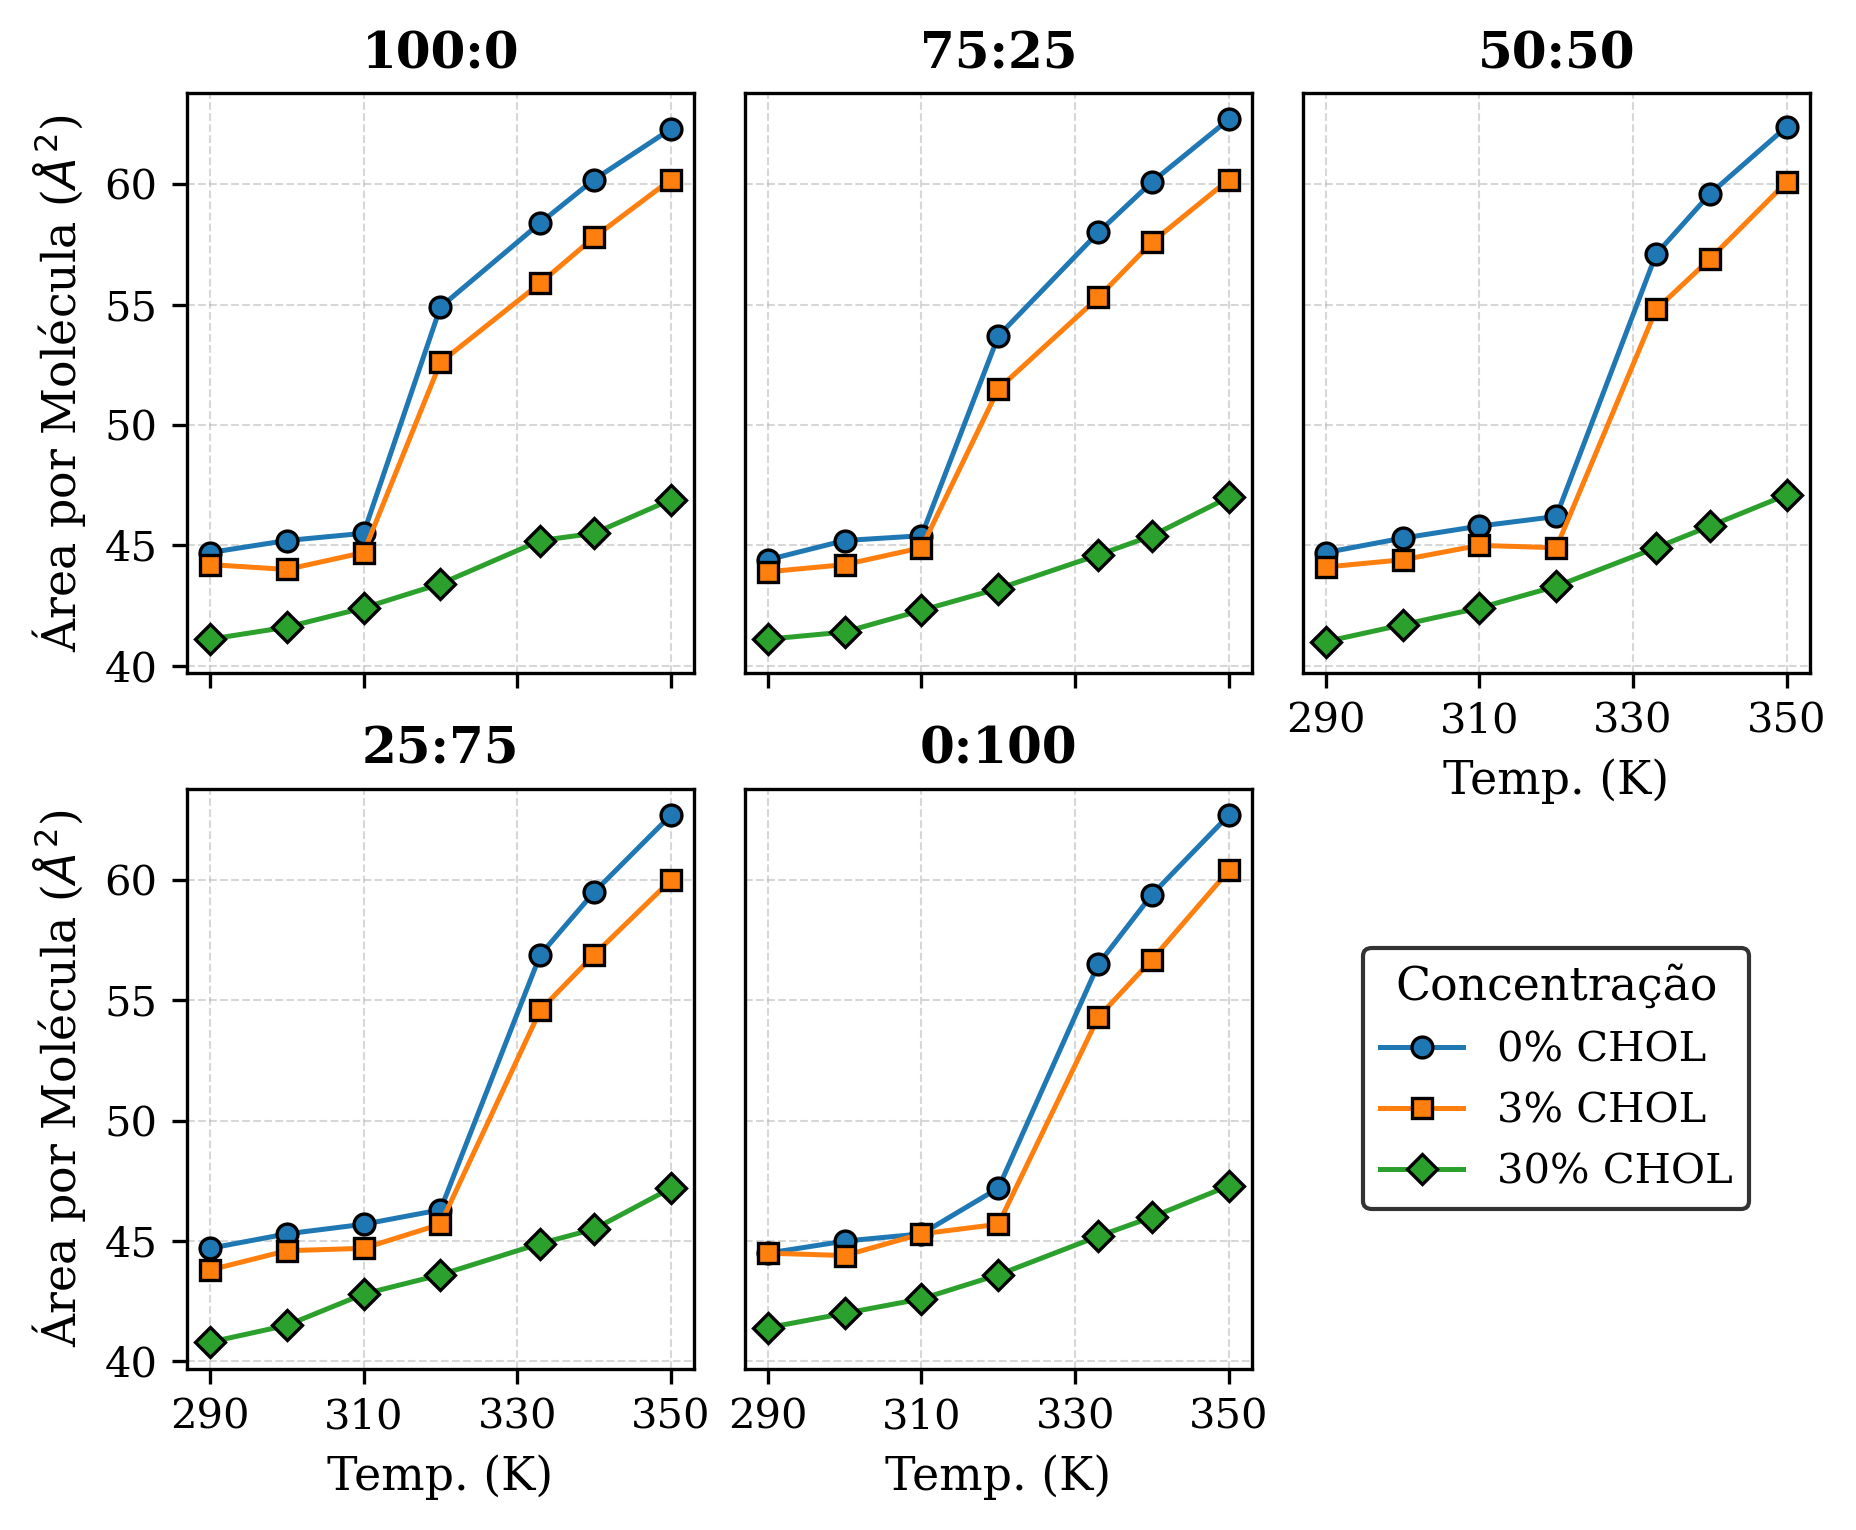
\includegraphics[width=\textwidth]{imagens/comparativo_chol_global.png}
    \caption{Mosaico da expansão térmica para misturas de DPPC/DSPC sob diferentes concentrações de colesterol (0\%, 3\% e 30\% em mol). Observa-se a supressão progressiva da transição de fase cooperativa em função do aumento da saturação por esterol.}
    \label{fig:mosaico_chol_global}
\end{figure}

A análise da área por molécula apresenta um decaimento à medida que a concentração de colesterol aumenta.  Este comportamento macroscópico ocorre por meio dos fosfolipídios que atuam como cordas flexíveis sujeitas a flutuações térmicas, enquanto a molécula de colesterol atua mecanicamente como uma haste rígida.  A presença do esterol suprime os graus de liberdade vibracionais das cadeias acílicas adjacentes, forçando o estiramento das mesmas e induzindo o achatamento da área lateral. 

No regime de baixa concentração (3\%), o colesterol atua como uma impureza que perturba o empacotamento da fase gel, mas preserva a transição para a fase fluida ($L_{\alpha}$). Em contrapartida, sob alta saturação (30\%), o efeito condensador torna-se absoluto. Para examinar a mecânica detalhada desta fase líquida-ordenada ($L_o$), a Figura \ref{fig:apl_chol_30} isola o perfil termotrópico do sistema com 30\% de esterol.

% --- Figura 4.9: Colesterol 30% (Efeito Condensador Linear) ---
\begin{figure}[htpb]
    \centering
    \includegraphics[width=\textwidth]{imagens/grafico_APL_CHOL\_30.png}
    \caption{Área média por molécula para o sistema com 30\% de colesterol. O efeito condensador lineariza a expansão térmica e anula a influência do comprimento da cadeia acílica, resultando na convergência das curvas para as diferentes misturas de DPPC/DSPC.}
    \label{fig:apl_chol_30}
\end{figure}

Neste regime, a expansão térmica torna-se linear. A restrição imposta pela haste rígida do colesterol suprime a transição de fase e sobrepõe-se à influência do comprimento da cadeia hidrocarbônica.

\subsubsection*{Efeito Combinado de Colesterol e Íons}

As membranas em meio biológico operam imersas em moleculas de água e eletrólitos, cuja presença dita interações interfaciais. Para aproximar o modelo deste cenário fisiológico, introduziu-se 0,15 M de NaCl, promovendo a ancoragem eletrostática e a blindagem dielétrica nas cabeças polares. O impacto global desta adição, combinada a diferentes níveis de saturação de colesterol, encontra-se documentado na Figura \ref{fig:mosaico_salino}.

% --- Figura 4.10: Mosaico Global do Colesterol com SAL ---
\begin{figure}[htpb]
    \centering
    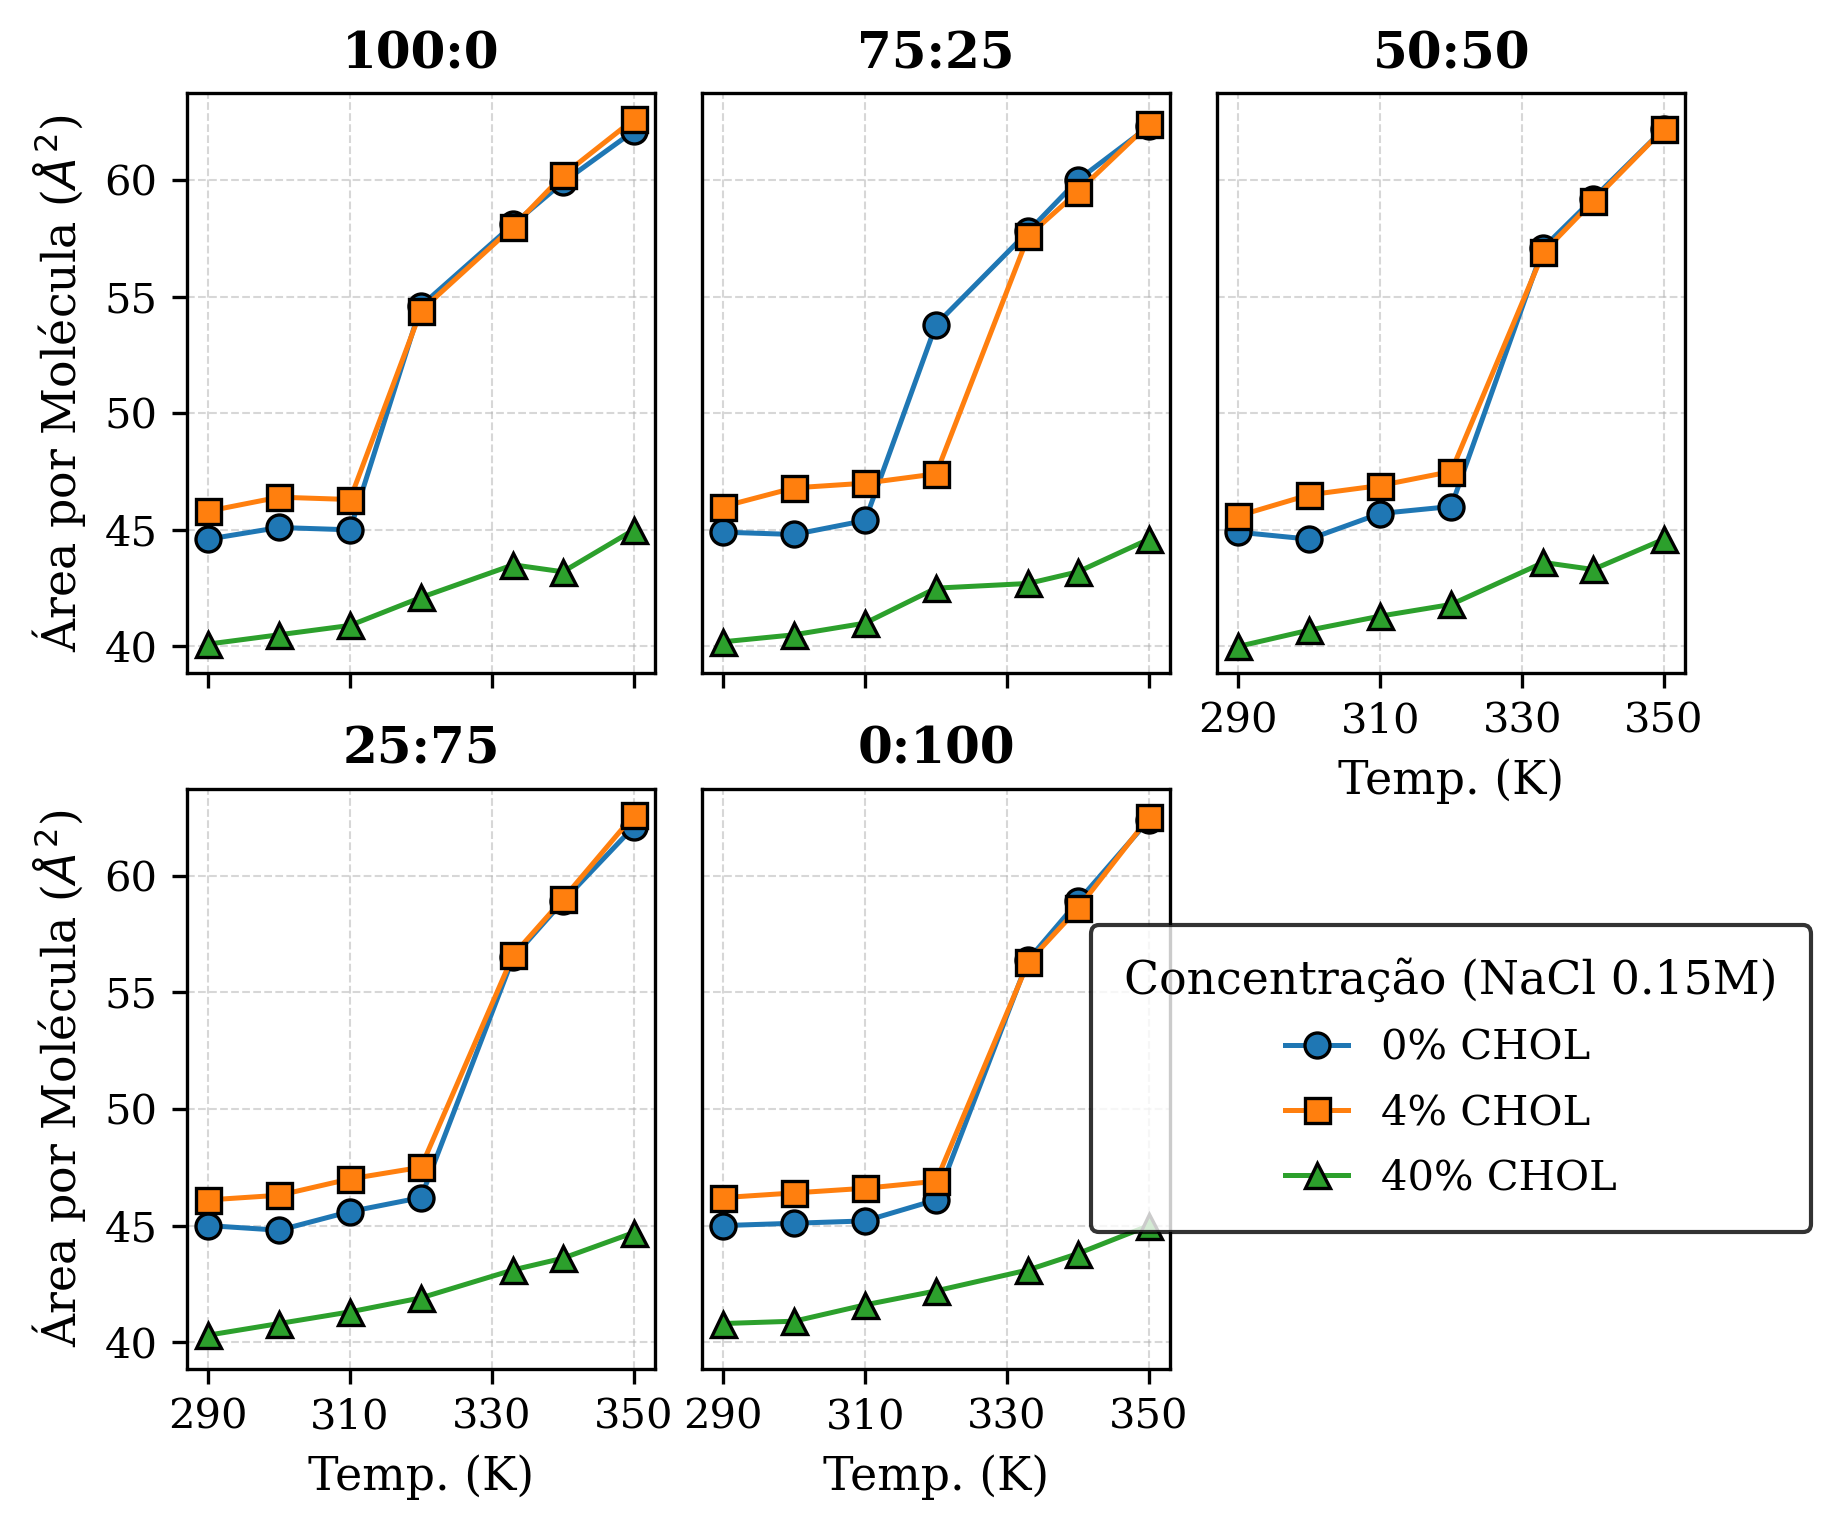
\includegraphics[width=\textwidth]{imagens/comparativo_global_salino.png}
    \caption{Mosaico termotrópico para as misturas binárias de DPPC/DSPC em meio salino fisiológico (0,15 M NaCl). Observa-se que a adição de alta concentração de colesterol (40\% em mol) sobrepõe-se à coordenação iônica interfacial, anulando a cooperatividade em todas as proporções estequiométricas.}
    \label{fig:mosaico_salino}
\end{figure}

O comportamento da simulação é baseado nas interações entre os beads. Em sistema puramente lipídico e com 4\% de colesterol, os íons exercem um papel estabilizador evidente: a coordenação dos cátions de sódio ($Na^+$) com os oxigênios carbonílicos favorece o empacotamento lateral, mantendo uma transição de fase de primeira ordem a aproximadamente 320 K. 

No entanto, a inserção de 40\% de colesterol impõe uma retificação física significativa. A dominância termomecânica do esterol induz a condensação acentuada das caudas flexíveis, achatando a curva termotrópica em todas as frações lipídicas (convergência para valores entre $43$ e $45$ \AA$^2$). Esta dinâmica demonstra que a rigidez imposta pela formação da fase $L_o$ anula a cooperatividade intrínseca da matriz lipídica, sobrepondo-se à ancoragem elétrica proporcionada pela rede salina.


% =====================================================================
% SECÇÃO 4.3 - FUNDAMENTOS TERMODINÂMICOS
% =====================================================================

\subsection{Análise Termodinâmica Global: Coulomb vs. Lennard-Jones}

Para fundamentar empiricamente o balanço termodinâmico global da caixa de simulação, definiu-se a Energia Total ($E_{Tot}$) como o somatório algébrico das contribuições não-covalentes globais ($E_{Tot} = E_{Coulomb} + E_{LJ}$). 

Uma vez que as parcelas de Coulomb e de Lennard-Jones consistem em variáveis derivadas das flutuações estatísticas intrínsecas ao campo de força, a propagação dessas variâncias exige um tratamento metrológico específico de acordo com as diretrizes e normativas adotadas na física experimental. A combinação dessas grandezas enquadra-se no cálculo da Incerteza Padrão Combinada ($u_c$) \cite{kallner2001uncertainty}. A sua magnitude final é determinada pelo cômputo da raiz quadrada da soma em quadratura das incertezas-padrão estatísticas originais:

\begin{equation}
    u_{c} = \sqrt{\left(\frac{\partial E_{Tot}}{\partial E_{Coulomb}} u_{Coulomb}\right)^2 + \left(\frac{\partial E_{Tot}}{\partial E_{LJ}} u_{LJ}\right)^2} = \sqrt{u_{Coulomb}^2 + u_{LJ}^2}
\end{equation}

Os resultados da Energia Total para todos os sistemas simulados encontram-se tabulados na Tabela \ref{tab:dados_brutos_energias} (Anexos).

A análise comparativa das energias eletrostáticas de Coulomb, Figura \ref{fig:coulomb_comparativo}) e das forças de Lennard-Jones, Figura \ref{fig:lj_comparativo}) permite distinguir os eixos termodinâmicos que governam a estabilidade da membrana. Os dados indicam que a interface polar e o núcleo apolar da bicamada respondem de forma distinta a mudanças térmicas e químicas.

Conforme a Figura \ref{fig:coulomb_comparativo}, as interações de Coulomb apresentam dependência da composição iônica do solvente e do grau de hidratação. Enquanto as membranas puras em meio sem sal exibem energias de Coulomb limitadas pelas interações entre os dipolos das cabeças zwitteriônicas, a adição de NaCl induz uma estabilização eletrostática expressiva. Este decréscimo energético decorre da coordenação específica de íons $Na^+$ com os grupos carbonílicos e fosfato das cabeças lipídicas, formando pontes eletrostáticas que conferem maior coesão à interface \cite{bockmann2003, javanainen2017}.

\begin{figure}[H]
    \centering
    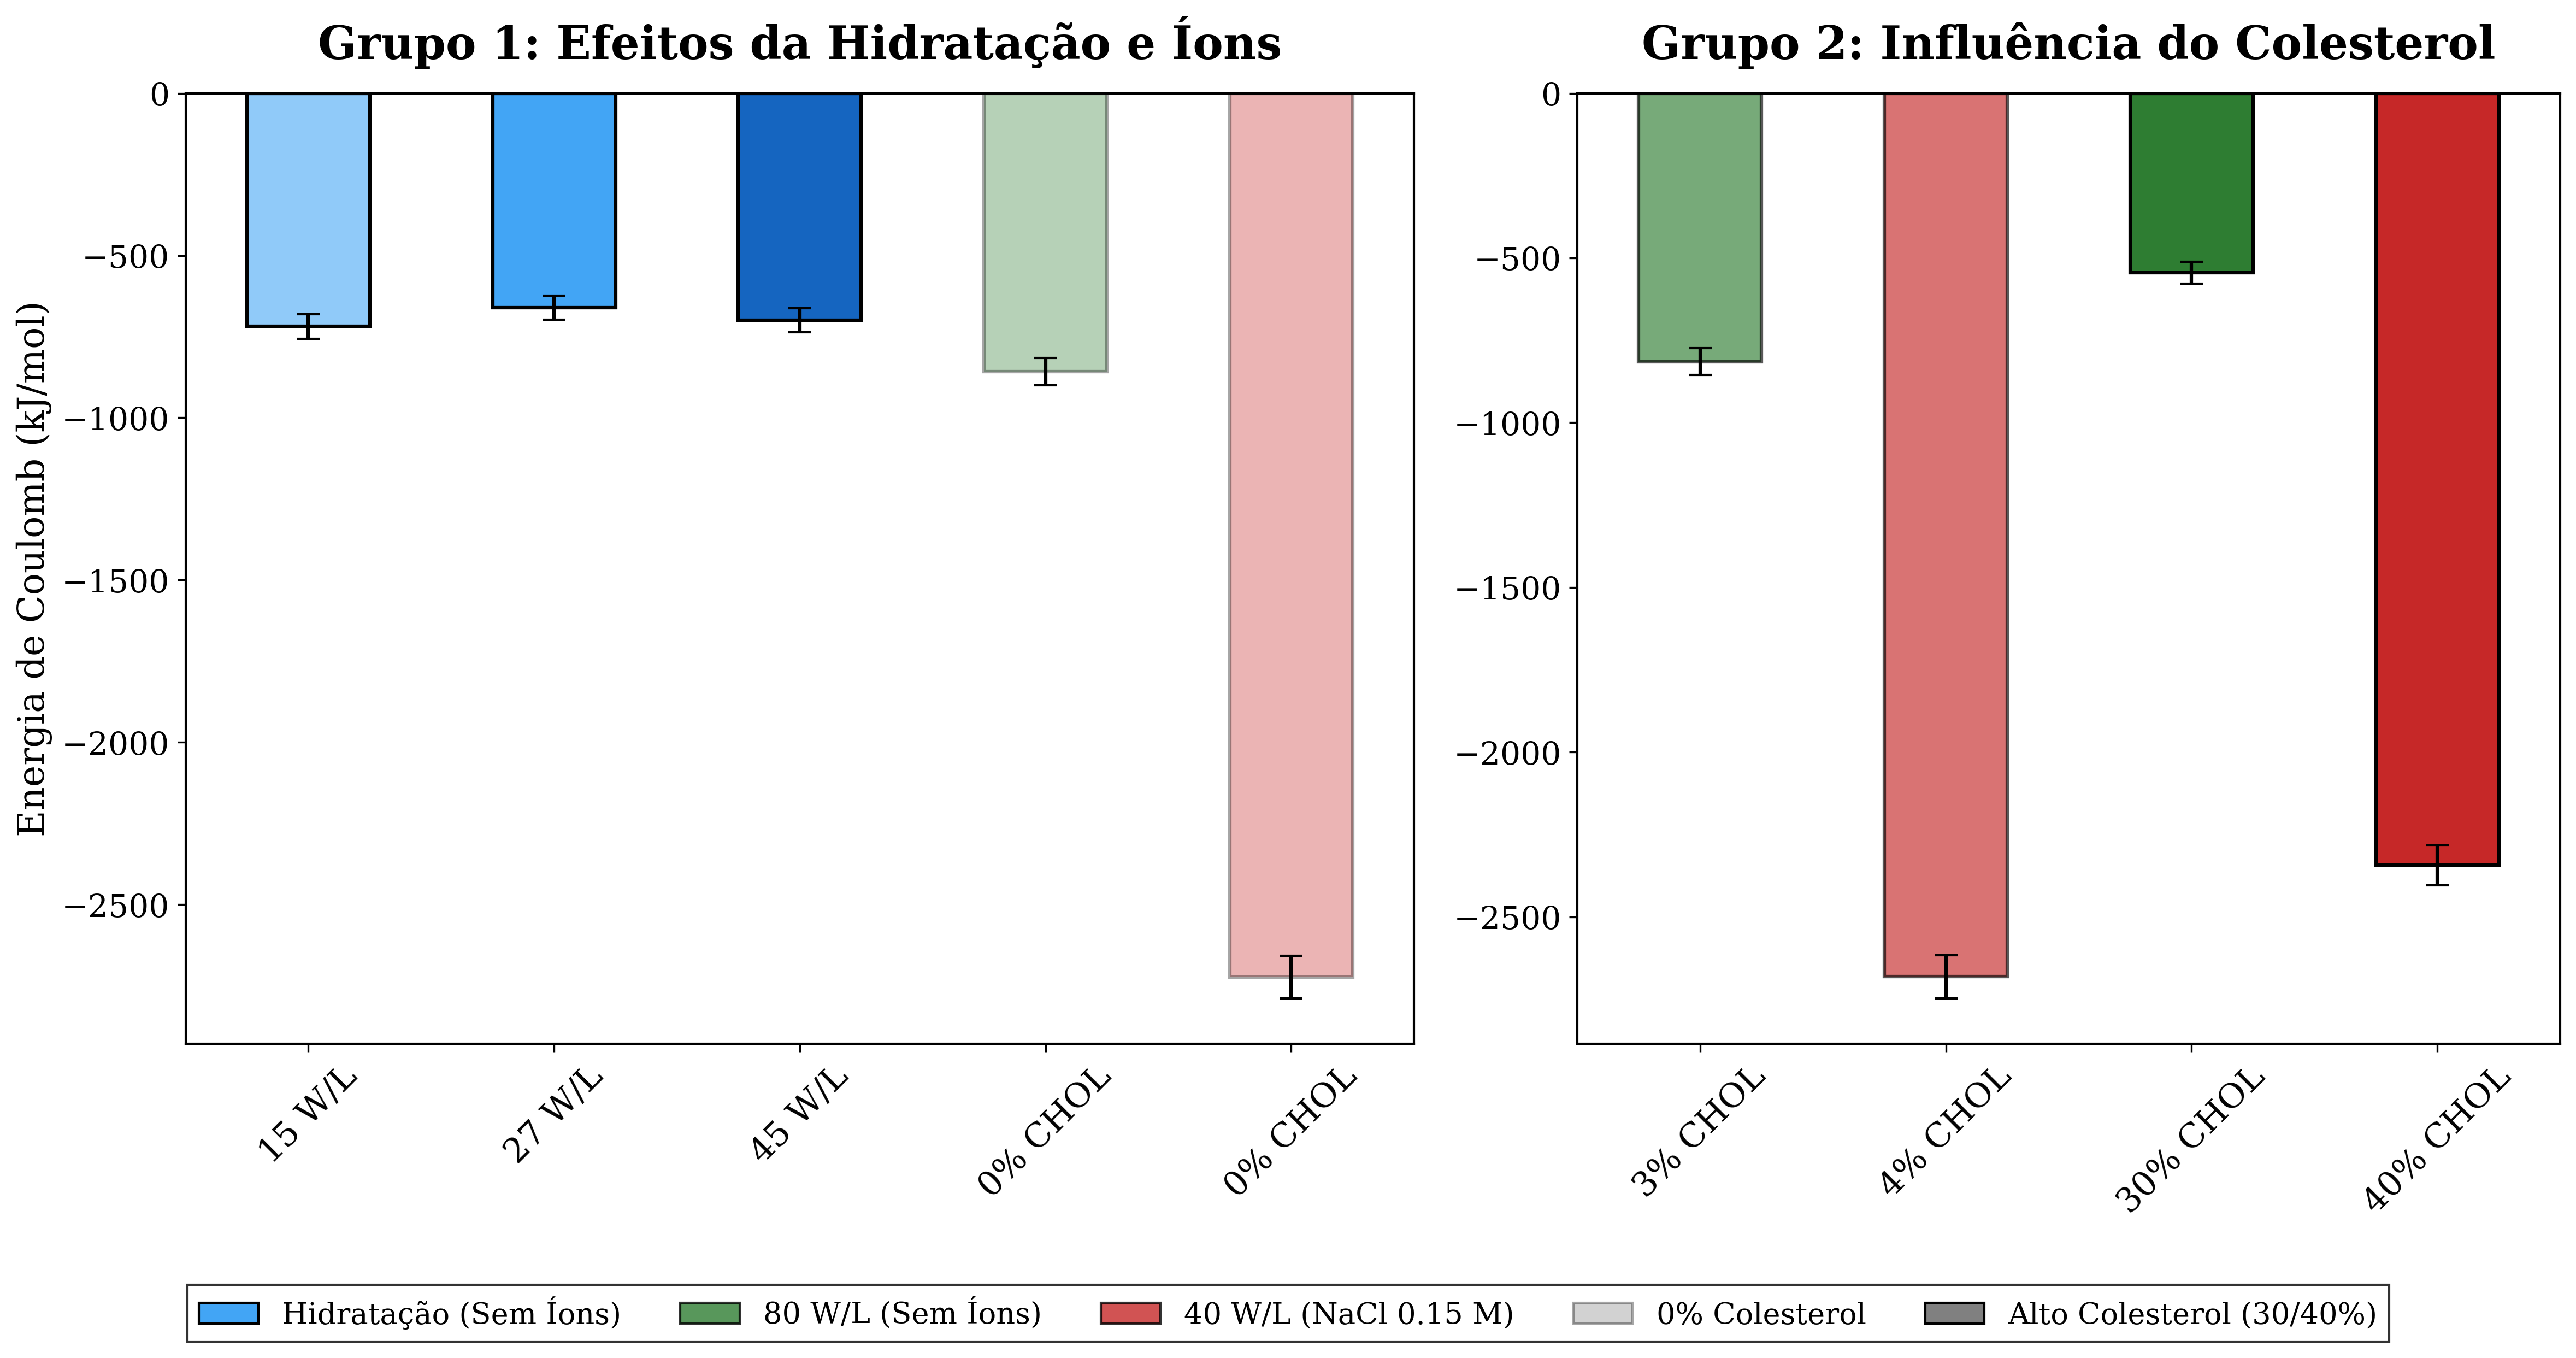
\includegraphics[width=0.9\textwidth]{imagens/comparativo_Coulomb_Exato.png}
    \caption{Energias eletrostáticas (Coulomb) médias. O Grupo 1 demonstra o impacto da hidratação, enquanto o sistema com NaCl (vermelho) evidencia a estabilização por coordenação iônica. No Grupo 2, o colesterol não altera significativamente o domínio eletrostático devido à sua neutralidade elétrica.}
    \label{fig:coulomb_comparativo}

    \vspace{0.8cm}

    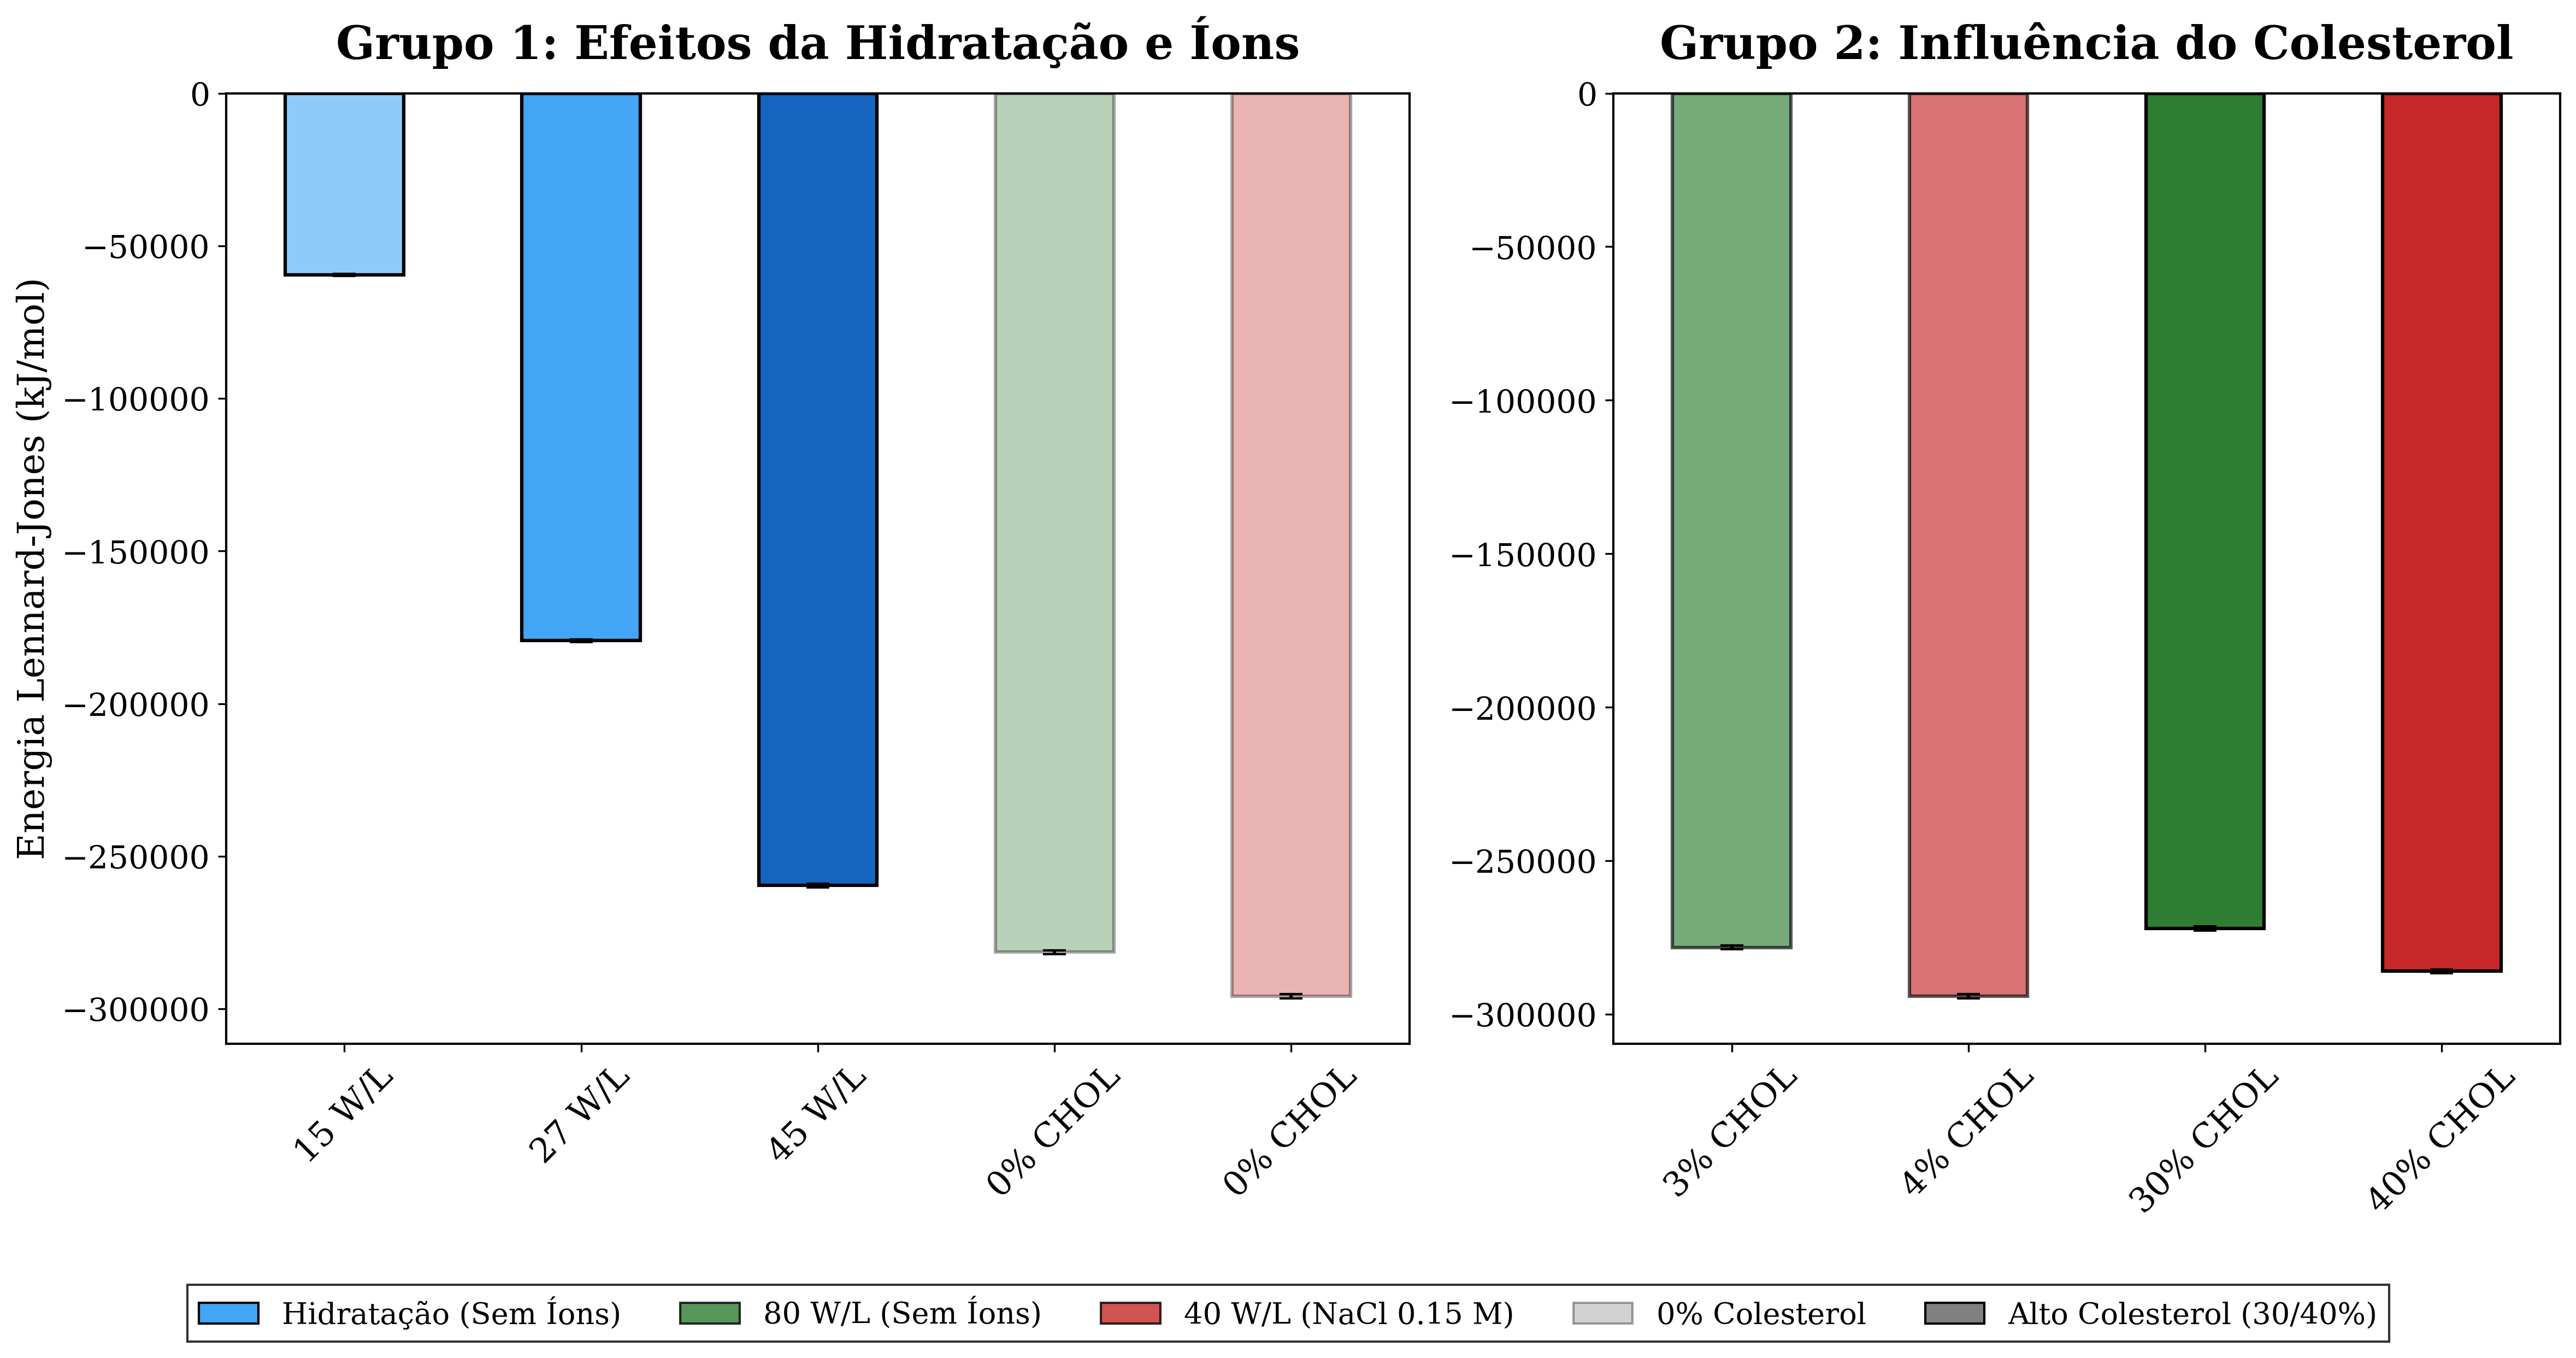
\includegraphics[width=0.9\textwidth]{imagens/comparativo_LJ_Exato.png}
    \caption{Energias de dispersão (Lennard-Jones) médias. O crescimento linear em degraus nos sistemas do Grupo 1, reflete a densidade do solvente. No Grupo 2, observa-se a estabilidade entálpica global: a condensação lateral induzida pelo colesterol não altera a energia de forma expressiva.}
    \label{fig:lj_comparativo}
\end{figure}

Em contrapartida, as forças de Lennard-Jones apresentam um perfil termodinâmico distinto, centrado na densidade de empacotamento. À esquerda da Figura \ref{fig:lj_comparativo}, observa-se uma variação linear da energia de dispersão com o aumento da hidratação, indicando que as contribuições LJ são ditadas majoritariamente pela rede de interações do solvente que permeia a interface.

A análise do Grupo 2 na Figura \ref{fig:lj_comparativo} mostra que a redução da APL induzida pelo colesterol não altera significativamente a energia de Lennard-Jones total da caixa. Este comportamento indica uma compensação entálpica eficiente: a perda das interações decorrente da expulsão de água da interface é compensada pelo ganho de contatos atrativos de van der Waals no núcleo hidrofóbico, decorrente do empacotamento das cadeias acílicas \cite{peccati2021enthalpy}.

Ao analisar os dados de energia dos sistemas com colesterol, observa-se que as energias globais de Coulomb e Lennard-Jones tornam-se menos negativas com o incremento da concentração do esterol. Este comportamento não reflete uma desestabilização estrutural interna da bicamada, mas sim um viés inerente à medição de propriedades nas simulações.

O somatório energético da caixa de simulação engloba as interações lipídio-lipídio, água-água e lipídio-água. A adição de colesterol ocasiona um efeito condensador, o qual reduz a APL e, por consequência geométrica, a área de contato total da interface polar. Esta compactação expulsa um volume significativo de água de hidratação primária. Somado a isso, a substituição dos lipídios DPPC e DSPC pelo colesterol reduz ainda mais a densidade de sítios de interação interfacial.

Portanto, a elevação dos valores globais de energia traduz a perda mecânica de contato entre a superfície da membrana e o solvente. Microscopicamente, no núcleo apolar da bicamada, o cenário é inverso: a inserção de esterol induz a conformação \textit{all-trans} das cadeias acílicas, maximizando o empacotamento. Este alinhamento torna a energia local de Lennard-Jones fortemente mais atrativa. É a magnitude dessa estabilização local lipídio-lipídio que garante a integridade e o ordenamento da fase $L_o$, assim a aparente penalidade energética do sistema global mascara um robusto ganho de coesão interna na membrana.

A energia de Lennard-Jones da caixa inteira variou de $\approx -304.000\text{ kJ/mol}$ no Controle para $\approx -290.000\text{ kJ/mol}$ a 40\% de Colesterol, uma diferença de $\approx 4,5\%$. Esta variação atesta que o ganho de atração molecular estabelecido no confinamento do núcleo hidrofóbico ($U \propto -1/r^6$) compensa o elevado débito da dessolvatação superficial. A membrana cede uma pequena fração da sua entalpia global para consolidar a rigidez mecânica, tornando a fase líquida-ordenada ($L_o$) termodinamicamente viável e protegendo a membrana de flutuações estruturais severas.

\vspace{1em}
\noindent\textbf{Fundamentação Energética da Metaestabilidade: A Barreira de Dessolvatação}

A investigação do comportamento termotrópico focada na evolução do modelo de DSPC sob alta hidratação (45 W/L), demonstra uma limitação da metodologia: o aprisionamento da matriz estrutural em um estado metaestável. Em temperaturas abaixo da transição, as simulações indicaram que a membrana de DSPC manteve sua área lateral em aproximadamente $61,5\text{ \AA}^2$. O sistema não atingiu a transição para a fase gel sólida ($L_\beta$), que exigiria uma compactação para valores próximos a $45,0\text{ \AA}^2$, transição esta observada apenas a partir de 310 K.

A justificativa para essa metaestabilidade, caracterizada pela inibição da nucleação cooperativa, baseia-se na necessidade energética para dessolvatação, refletida nas variações das energias de Lennard-Jones observadas \cite{kowalik2015}. Quando a membrana permanece dilatada, as moléculas de água e íons interagem com os grupos polares das cabeças lipídicas. Esta hidratação estabelece um conjunto de interações atrativas favorável entalpicamente. Para que a membrana cristalize na fase gel, é necessário que ocorra uma compressão lateral. Remover essa estrutura atrativa consolidada pelo solvente está ligada a Força de Repulsão por Hidratação.

A mecânica desta repulsão hídrica gera obstáculos estruturais da transição de fase $L_\alpha \rightarrow L_\beta$. Protocolos experimentais de desidratação controlada demonstraram que a remoção de água interfacial atua como o principal fator necessário para induzir o reordenamento geométrico das caudas hidrofóbicas dos lipídios. A fase previamente desordenada adota características estereoquímicas de maior densidade e rigidez, próprias da fase gel \cite{krok2024}.

Portanto, os dados sugerem que a metaestabilidade observada para o DSPC está ligada ao sistema em romper a sua camada de hidratação interfacial favorável. O sistema não adquire o empacotamento gel porque tal processo exigiria uma quebra das interações com a água, acarretando uma barreira entálpica.


\vspace{1em}
\noindent\textbf{Barreira de Dessolvatação}

A barreira de dessolvatação e a consequente metaestabilidade observadas nas simulações podem ser quantificadas através da termodinâmica dos estados, utilizando o sistema de hidratação intermediária (27W\_L) como modelo estatístico. Diferente do regime de alta hidratação (que apresenta metastabilidade apenas para o sistema puro), o regime 27W\_L oferece robustez analítica superior ao exibir cinco pontos de retenção distribuídos em duas estequiometrias distintas: no DSPC puro (0:100) e na mistura rica em DSPC (25:75).

A literatura ressalta que o balanço fino das interações não covalentes, especialmente a calibração das forças de dispersão de Lennard-Jones, é o principal motor para o empacotamento termodinamicamente correto das cadeias hidrocarbônicas \cite{liu2012}. Utilizando os dados gerados, na Tabela \ref{tab:dados_brutos_energias} do Anexo, é possível calcular a energia associada a esta barreira. A diferença entre a energia global de Lennard-Jones no estado mestaestável, quando a membrana está expandida, e a fase gel quantifica a magnitude do "custo entálpico" exigido do sistema para afastar a água interfacial.

Para a mistura 25:75 (DPPC:DSPC), o sistema transita do estado metaestável a 300 K para a fase gel em 310 K. A energia global de Lennard-Jones salta de $-198.860,0$ kJ/mol para $-178.349,7$ kJ/mol. Esta variação resulta em um custo de dessolvatação de $+102,6$ kJ/mol por cada um dos 200 lipídios da caixa. 

Para o sistema de DSPC puro (0:100), que cristaliza apenas a 320 K ($-176.762,1$ kJ/mol), as barreiras entálpicas mensuradas a partir dos estados metaestáveis a 290 K, 300 K e 310 K foram de $+121,0$, $+112,5$ e $+102,5$ kJ/mol por lipídio, respectivamente, consolidando um custo entálpico médio de $\approx +112,0$ kJ/mol por molécula.

Esta análise comprova que a barreira de nucleação é proporcional ao volume de solvente disponível. Enquanto no sistema de hidratação 45W\_L a penalidade entálpica média atinge valores de até $\approx +188,8$ kJ/mol por molécula, a redução do volume de água livre no sistema 27W\_L fez com que a barreira energética média global caísse para $\approx +109,0$ kJ/mol por lipídio. A magnitude dessa barreira evidencia a assimetria fundamental entre a água biológica e a água do modelo CG \cite{ref_langmuir_2024}. 

Na temperatura de 300 K, a energia térmica de flutuação ($k_B T$) é de $\approx 2,5$ kJ/mol. Exigir uma energia livre interfacial dessa magnitude equivale a impor uma barreira de $\approx 75 \ k_B T$. Pela Equação de Arrhenius, a probabilidade de um microestado reunir espontaneamente essa quantidade de energia térmica é estatisticamente nula. Na natureza observável, a repulsão hídrica é rapidamente contornada porque a água se difunde e reorganiza, quebrando e refazendo pontes de hidrogênio direcionais; o curto déficit entálpico superficial é amplamente compensado pelo massivo ganho de Entropia rotacional e translacional ($+T\Delta S$) ao retornar ao solvente livre (\textit{bulk}). 

O campo de força Martini 3, contudo, aplica um mapeamento 4:1 que funde quatro moleculas de água em uma única esfera, suprimindo a direcionalidade quântica e a entropia rotacional.  Consequentemente, o modelo transforma um complexo movimento do sistema, modulado pela entropia, numa barreira entálpica na membrana. A atração transversal nas cadeias acílicas não consegue superar espontaneamente esta barreira superestimada, mantendo a matriz de lipídios no estado metaestável.

A conformação geométrica inerente a cada lipídio é confirmada no modelo, com as parametrizações implementadas. Fosfolipídios saturados possuem uma topologia essencialmente cilíndrica, o que favorece a formação de um arranjo lamelar compactado \cite{lee2022}. Contudo, a água aprisionada entre os grupos polares dilatados gera uma forte repulsão estérica e de hidratação, que age fisicamente como a barreira entálpica calculada acima.

\vspace{1em}
\noindent\textbf{Capacidade Calorífica}

Além da barreira entálpica de nucleação, os dados extraídos do regime de hidratação intermediária (27W\_L) permitem a quantificação de uma segunda propriedade termodinâmica fundamental: a Capacidade Calorífica à pressão constante ($C_p = \Delta E / \Delta T$). O acompanhamento da energia no estado metaestável antes da transição de fase mostra como o encurtamento da cadeia acílica em uma fração dos lipídios altera a absorção de energia do sistema (Tabela \ref{tab:dados_brutos_energias} do Anexo).

Para o sistema de DSPC puro, a variação energética de Lennard-Jones dentro da zona metaestável (290 K a 310 K) resultou em um $C_p$ aparente médio de $\approx 0,92$ kJ/mol/K. Na análise da mistura 25:75 (DPPC:DSPC), houve redução do $C_p$ da mistura metaestável (entre 290 K e 300 K) para $\approx 0,68$ kJ/mol/K. Esta correlação direta entre o encurtamento da cadeia e a queda da capacidade calorífica valida que a entalpia de empacotamento e a capacidade calorífica de fosfolipídios são medidas dependentes do mapeamento dos diferentes tamanhos de beads. 

Sob a ótica da mecânica estatística, a diminuição da capacidade calorífica no sistema misto reflete esta constatação, a redução da superfície hidrofóbica faz com que o sistema possua menos graus de liberdade para dissipar a energia térmica em excitações vibracionais. Consequentemente, a energia térmica fornecida $(k_B T)$ é transferida de forma mais eficiente para as flutuações coordenadas que formam o núcleo crítico de cristalização.

Isso explica o comportamento observado nas trajetórias: enquanto o DSPC puro, com sua maior área apolar ($C_p \approx 0,92$ kJ/mol/K), utiliza a energia térmica internamente e permanece retido na zona metaestável até 320 K, a mistura com apenas 25\% de cadeias mais curtas ($C_p \approx 0,68$ kJ/mol/K) otimiza o uso da energia e consegue superar a barreira de dessolvatação a 310 K.

\begin{figure}[H]
    \centering
    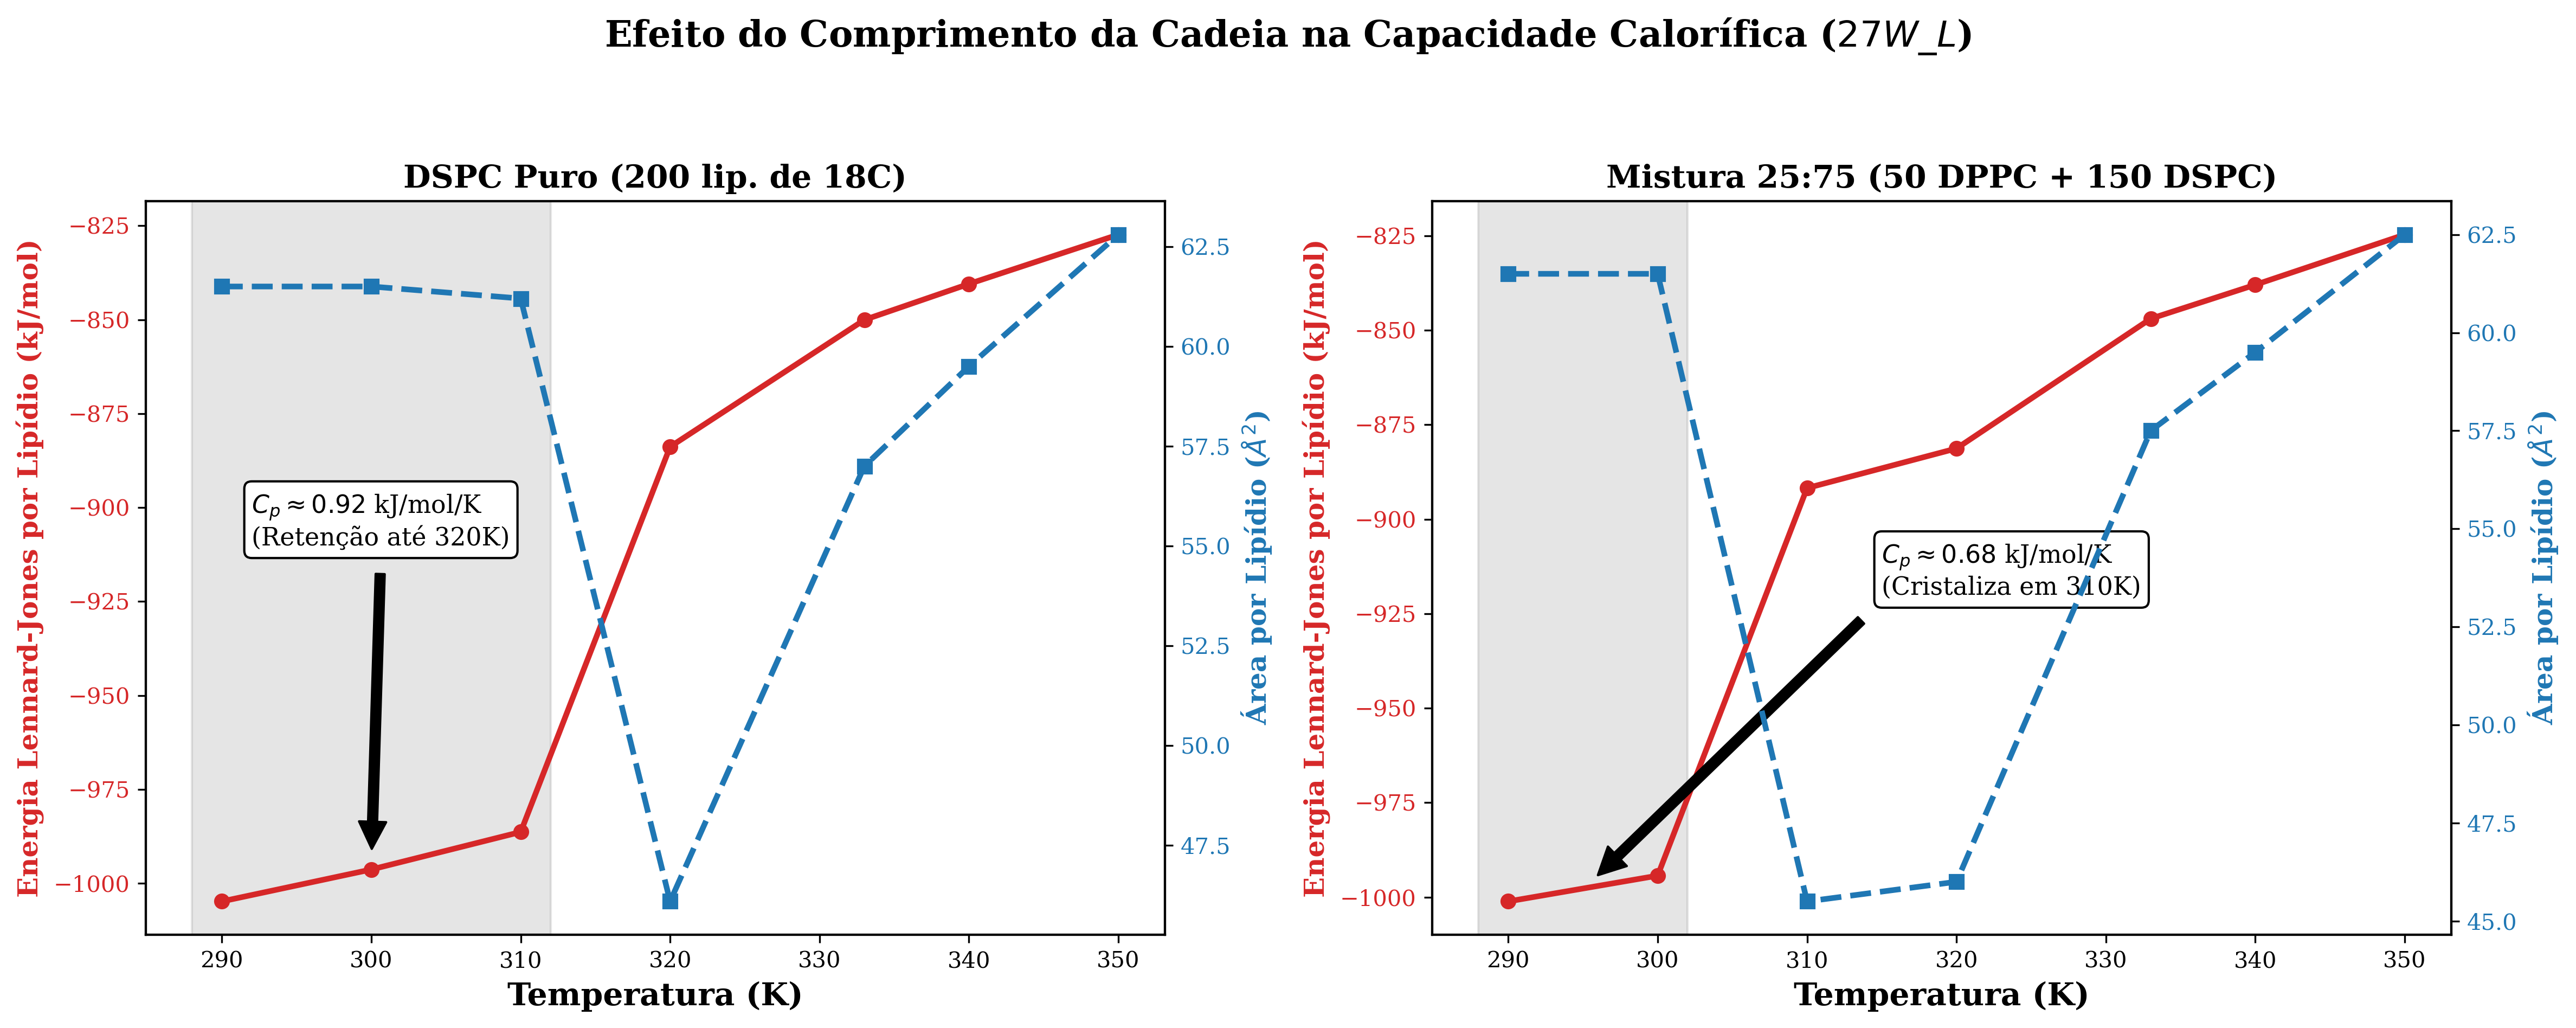
\includegraphics[width=\textwidth]{imagens/grafico_cp_27w.png}
    \caption{Comparativo termodinâmico da Capacidade Calorífica ($C_p$) sob hidratação de 27W\_L). As zonas em cinza delimitam o estado metaestável. À esquerda, o sistema de DSPC puro apresenta $C_p \approx 0,92$ kJ/mol/K. À direita, a substituição de 50 lipídios de DSPC por DPPC reduz a capacidade de dissipação térmica do sistema ($C_p \approx 0,68$ kJ/mol/K), permitindo que a energia seja utilizada de forma mais cooperativa, antecipando a nucleação da fase gel para 310 K.}
    \label{fig:capacidade_calorifica_27w}
\end{figure}

\vspace{1em}
\noindent\textbf{Permuta Entálpica e a Dinâmica de Compensação do Colesterol}

A inspeção da Tabela 5.1 fornece informações da forma como a membrana responde a mudança composicional: ocorre uma troca direta entre os domínios de energia. Foi observado que a substituição de fosfolipídios por concentrações elevadas de colesterol (como nos sistemas CHOL\_30) resulta em um enfraquecimento substancial do poço de potencial de Coulomb. Tomando a matriz de DSPC puro a 310 K como referência, a energia eletrostática decai de $-943,5$ kJ/mol (ausência de esterol) para $-565,7$ kJ/mol (com 30\% de colesterol). 

Esta perda expressiva de coesão eletrostática justifica-se pela arquitetura molecular do colesterol, que exibe apenas um grupo hidroxila ($-\text{OH}$). Para evitar o colapso estrutural frente à perda combinada de entropia vibracional e de atração de Coulomb interfacial, a membrana compensa a sua estabilidade no núcleo apolar. A condensação lateral induzida pelo colesterol força uma aproximação radial das cadeias hidrocarbônicas, maximizando os contatos de Lennard-Jones no interior da bicamada. Portanto, a membrana lipídica com colesterol é um sistema auto-regulável que cede as interações polares com o solvente na interface para obter a estabilização, sustentando assim o empacotamento denso da fase líquida-ordenada ($L_o$).

% =====================================================================
% SECÇÃO 4.4 - ANÁLISE MORFOLÓGICA (VMD)
% =====================================================================

\subsection{Topologia Interfacial e Empacotamento Hidrofóbico: Análise Morfológica}

As métricas termodinâmicas e estruturais observadas refletem microestados conformacionais que podem ser diretamente validados através da inspeção topológica. Para este fim, procedeu-se à análise visual das trajetórias moleculares utilizando o \textit{Visual Molecular Dynamics} (VMD), permitindo a correlação entre o perfil termotrópico e o arranjo espacial das cadeias e do solvente na nanoescala.

A análise estrutural da bicamada lipídica composta por DPPC/DSPC/Colesterol (na proporção 50:50 para os fosfolipídios, com 40\% em mol de colesterol) a 333 K mostra a formação de um sistema lamelar estável ao final da etapa de produção. A inspeção visual das trajetórias demonstra a ausência de separação macroscópica de fases (formação de grandes domínios isolados), evidenciando uma mistura homogênea em ambos os folhetos da membrana.

Essa estabilidade pode ser acompanhada na Figura \ref{fig:mosaico_dinamico}, que apresenta, além da perspectiva lateral, uma sequência de quadros (\textit{frames}) extraídos da simulação. A evolução temporal evidencia a constância do Efeito Condensador: as moléculas de colesterol (em amarelo) não formam aglomerados segregados, mas permanecem dinamicamente intercaladas entre as cadeias acílicas, garantindo um empacotamento denso e contínuo característico da fase líquida-ordenada ($L_o$).

\begin{figure}[H]
    \centering
    % ================= PRIMEIRA LINHA (4 imagens) =================
    \begin{subfigure}[b]{0.24\textwidth}
        \centering
        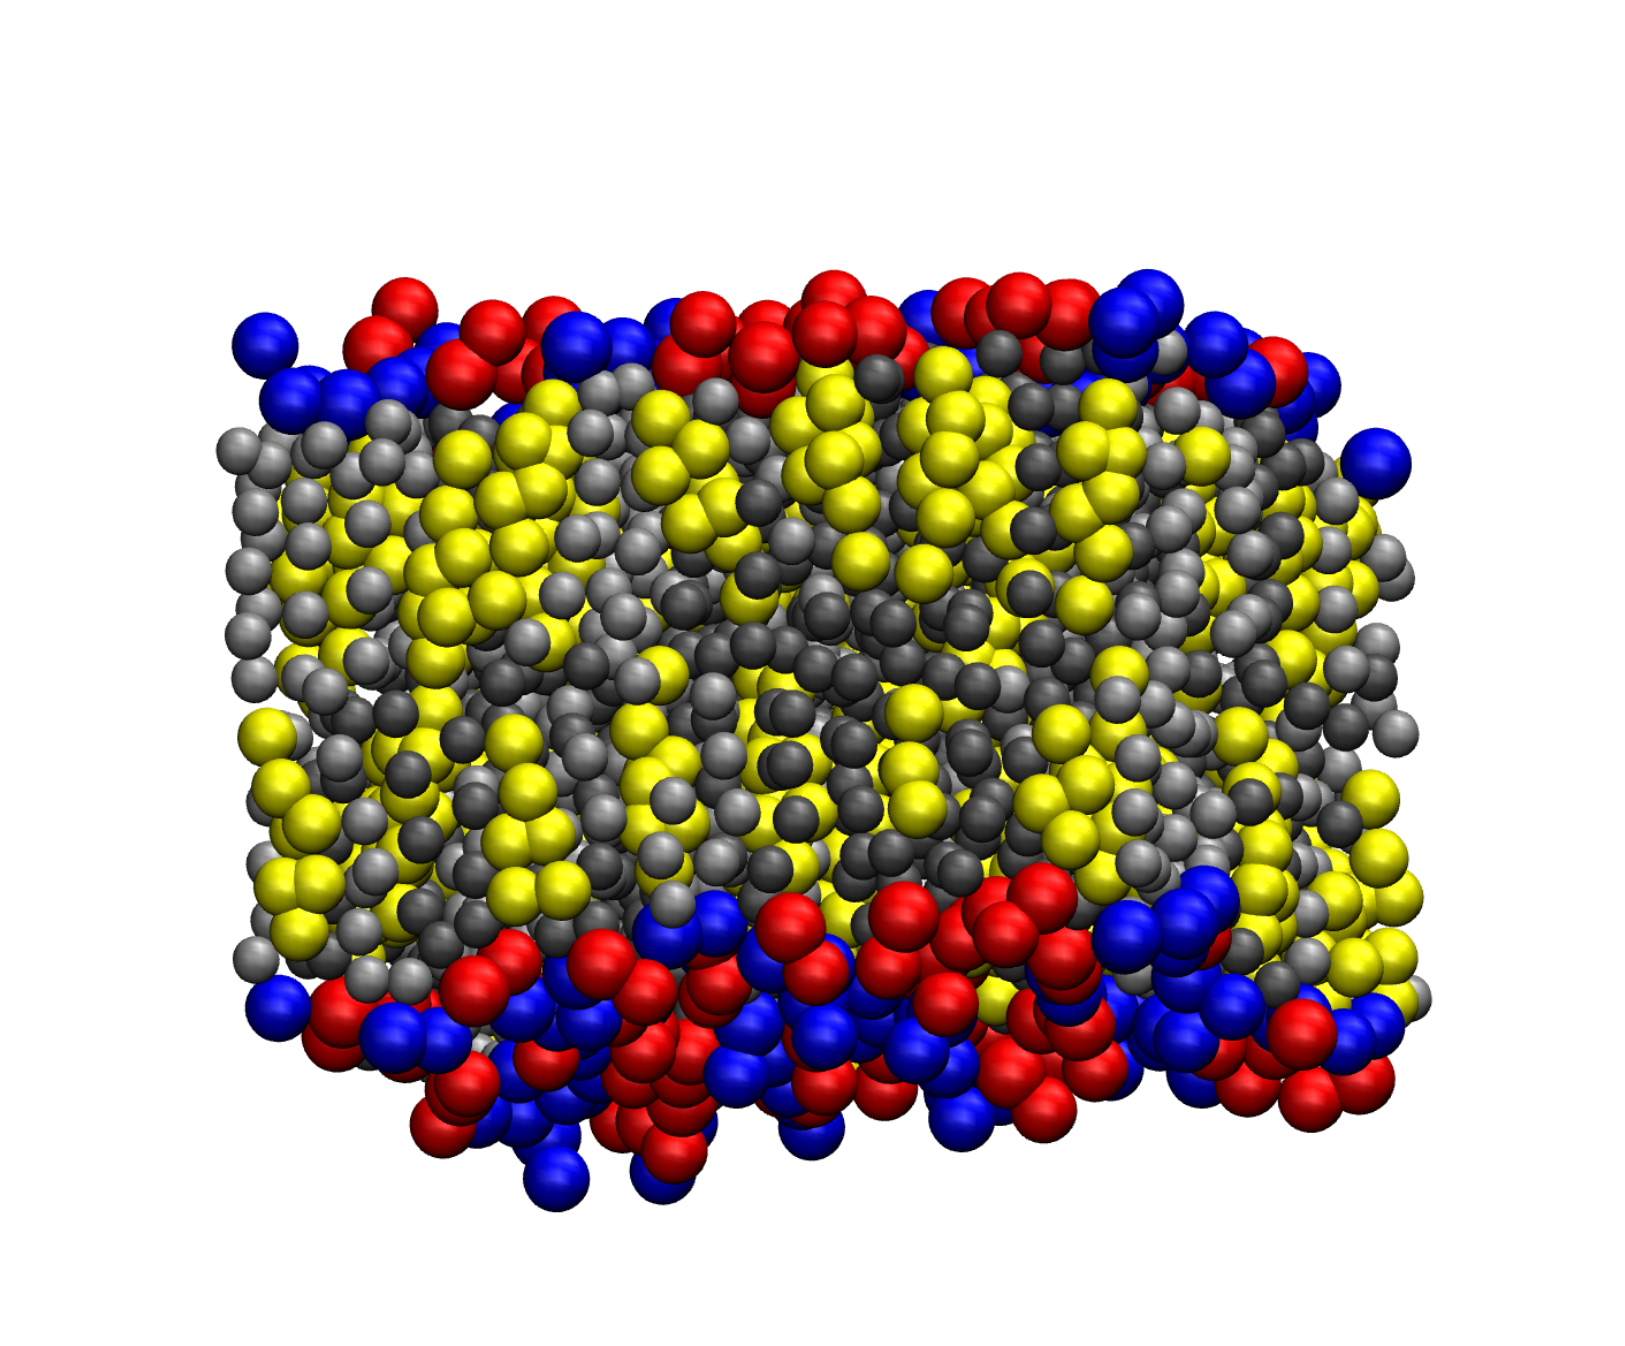
\includegraphics[width=\textwidth]{imagens/img1.jpg}
        \caption{Vista lateral}
    \end{subfigure}
    \hfill
    \begin{subfigure}[b]{0.24\textwidth}
        \centering
        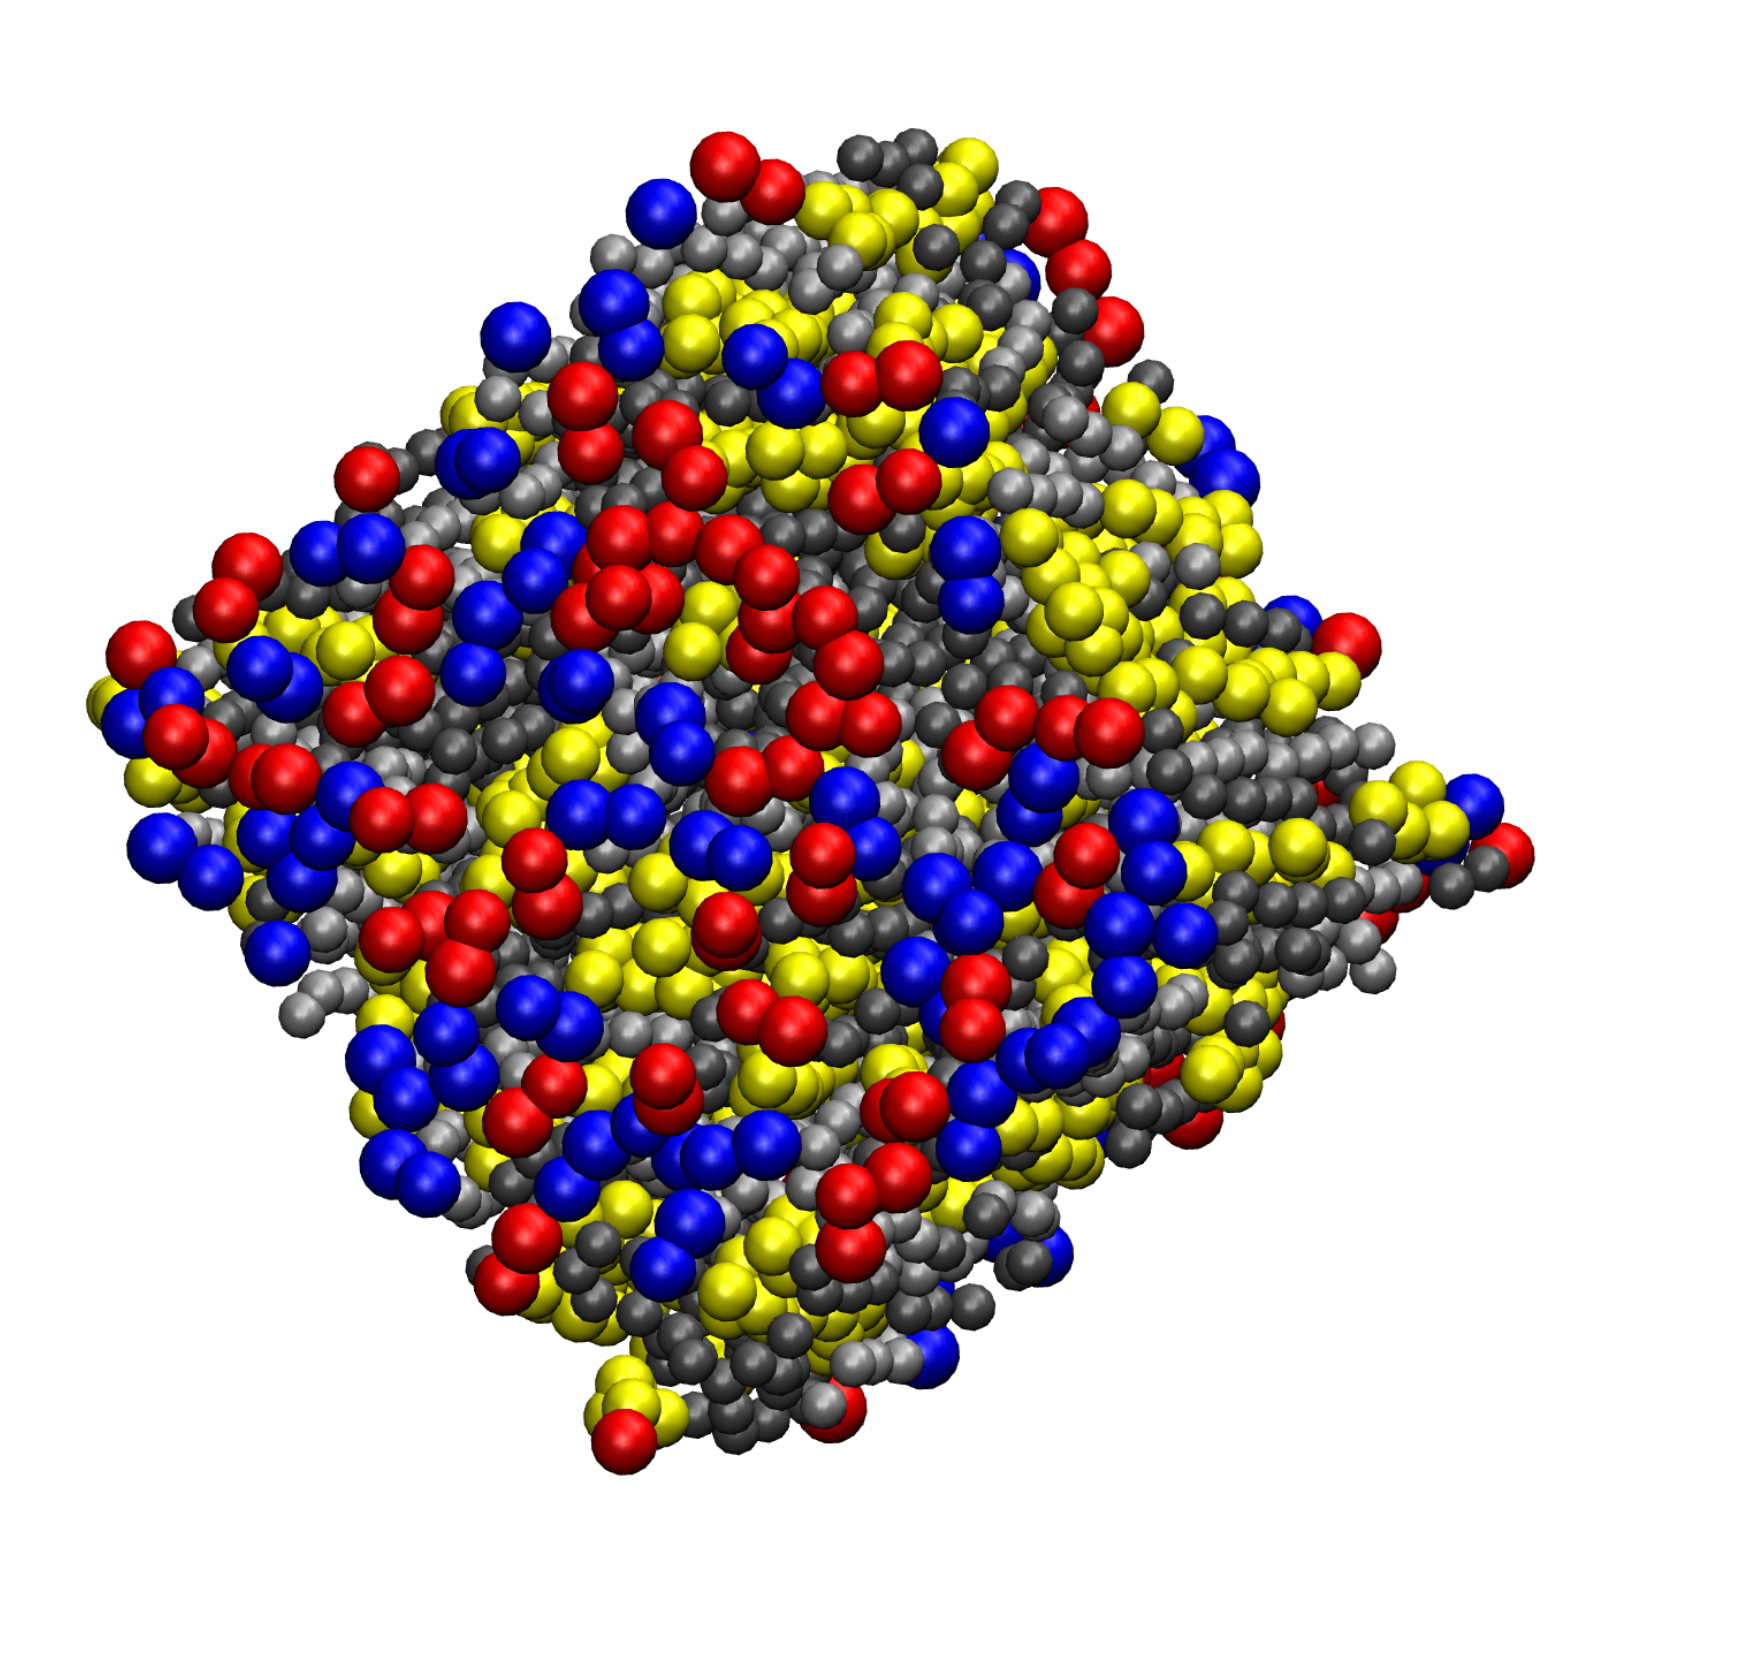
\includegraphics[width=\textwidth]{imagens/img3.jpg} 
        \caption{Frame $t_1$}
    \end{subfigure}
    \hfill
    \begin{subfigure}[b]{0.24\textwidth}
        \centering
        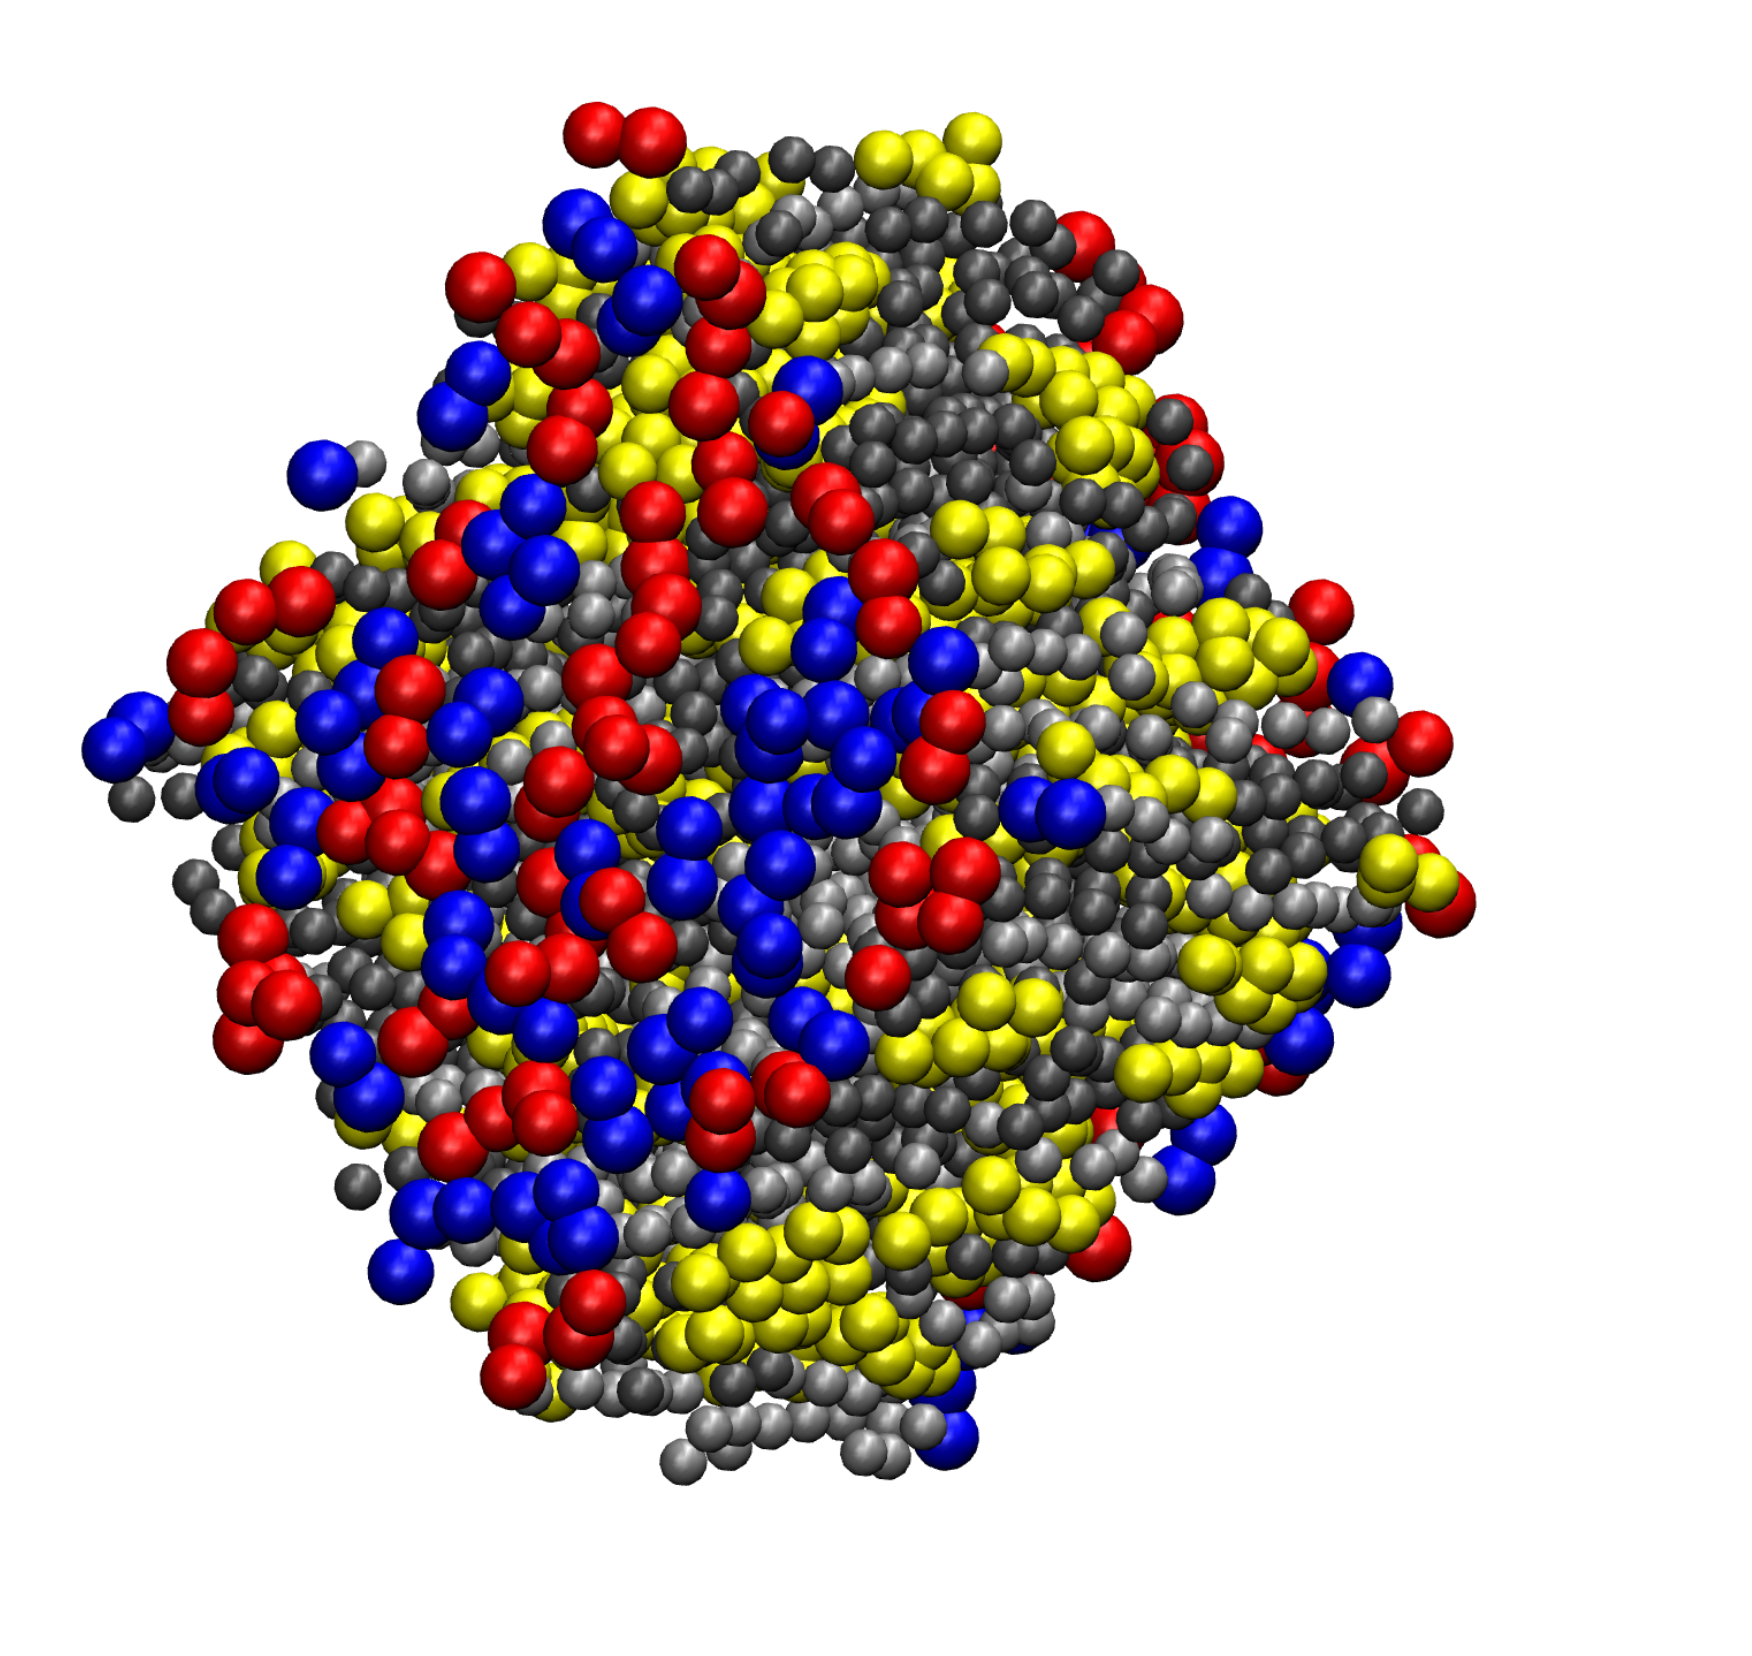
\includegraphics[width=\textwidth]{imagens/img4.jpg}
        \caption{Frame $t_2$}
    \end{subfigure}
    \hfill
    \begin{subfigure}[b]{0.24\textwidth}
        \centering
        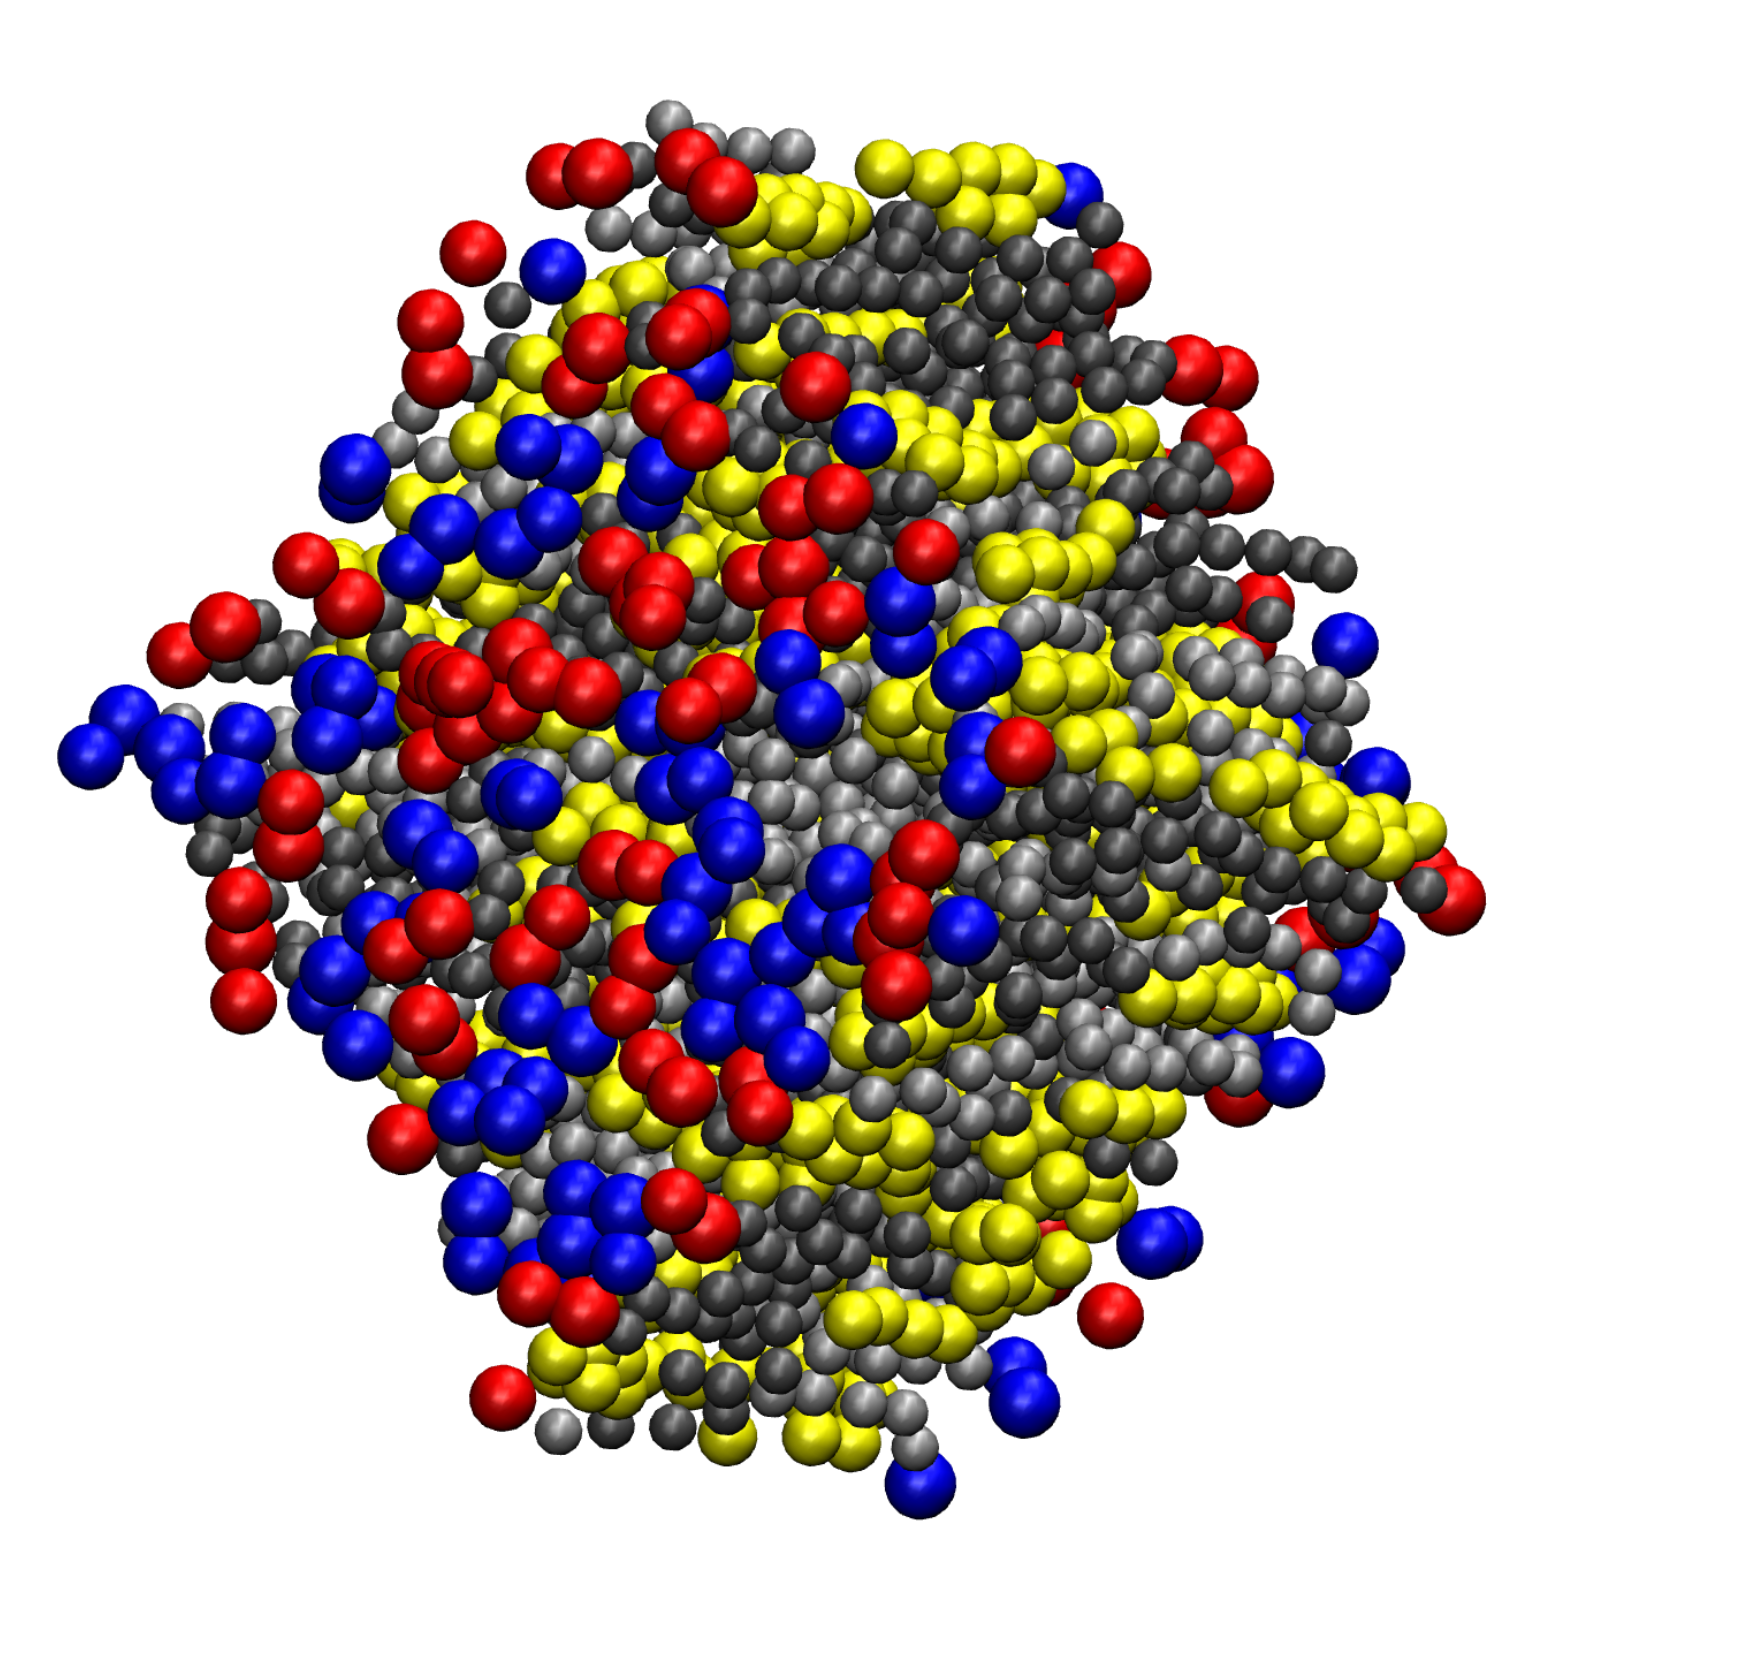
\includegraphics[width=\textwidth]{imagens/img5.jpg}
        \caption{Frame $t_3$}
    \end{subfigure}

    \vspace{0.4cm} 

    % ================= SEGUNDA LINHA (4 imagens) =================
    \begin{subfigure}[b]{0.24\textwidth}
        \centering
        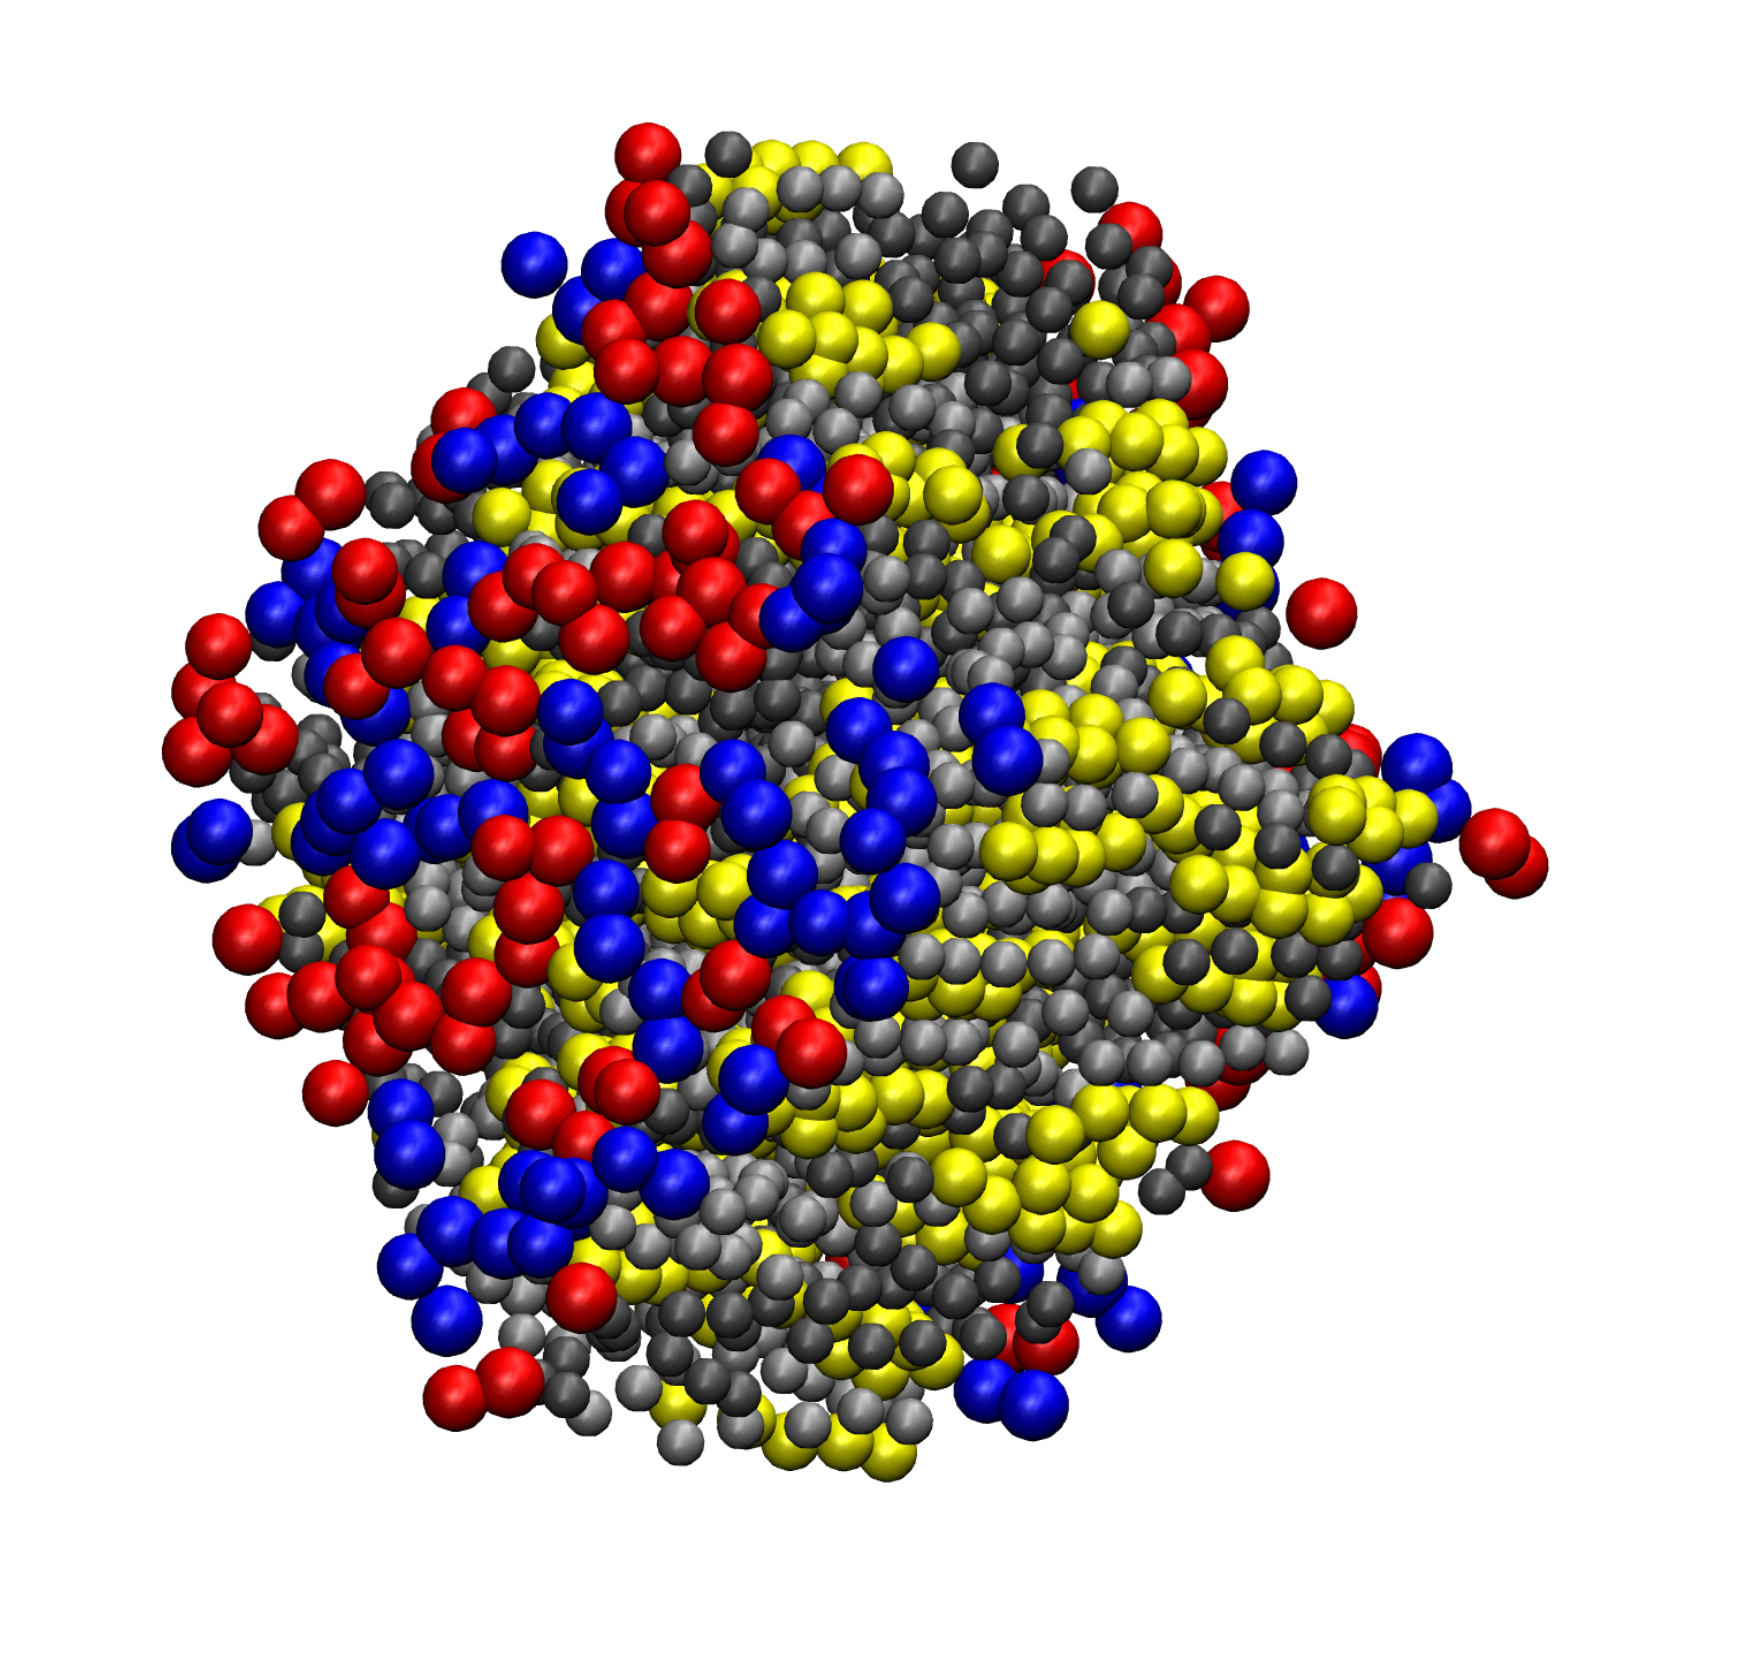
\includegraphics[width=\textwidth]{imagens/img6.jpg}
        \caption{Frame $t_4$}
    \end{subfigure}
    \hfill
    \begin{subfigure}[b]{0.24\textwidth}
        \centering
        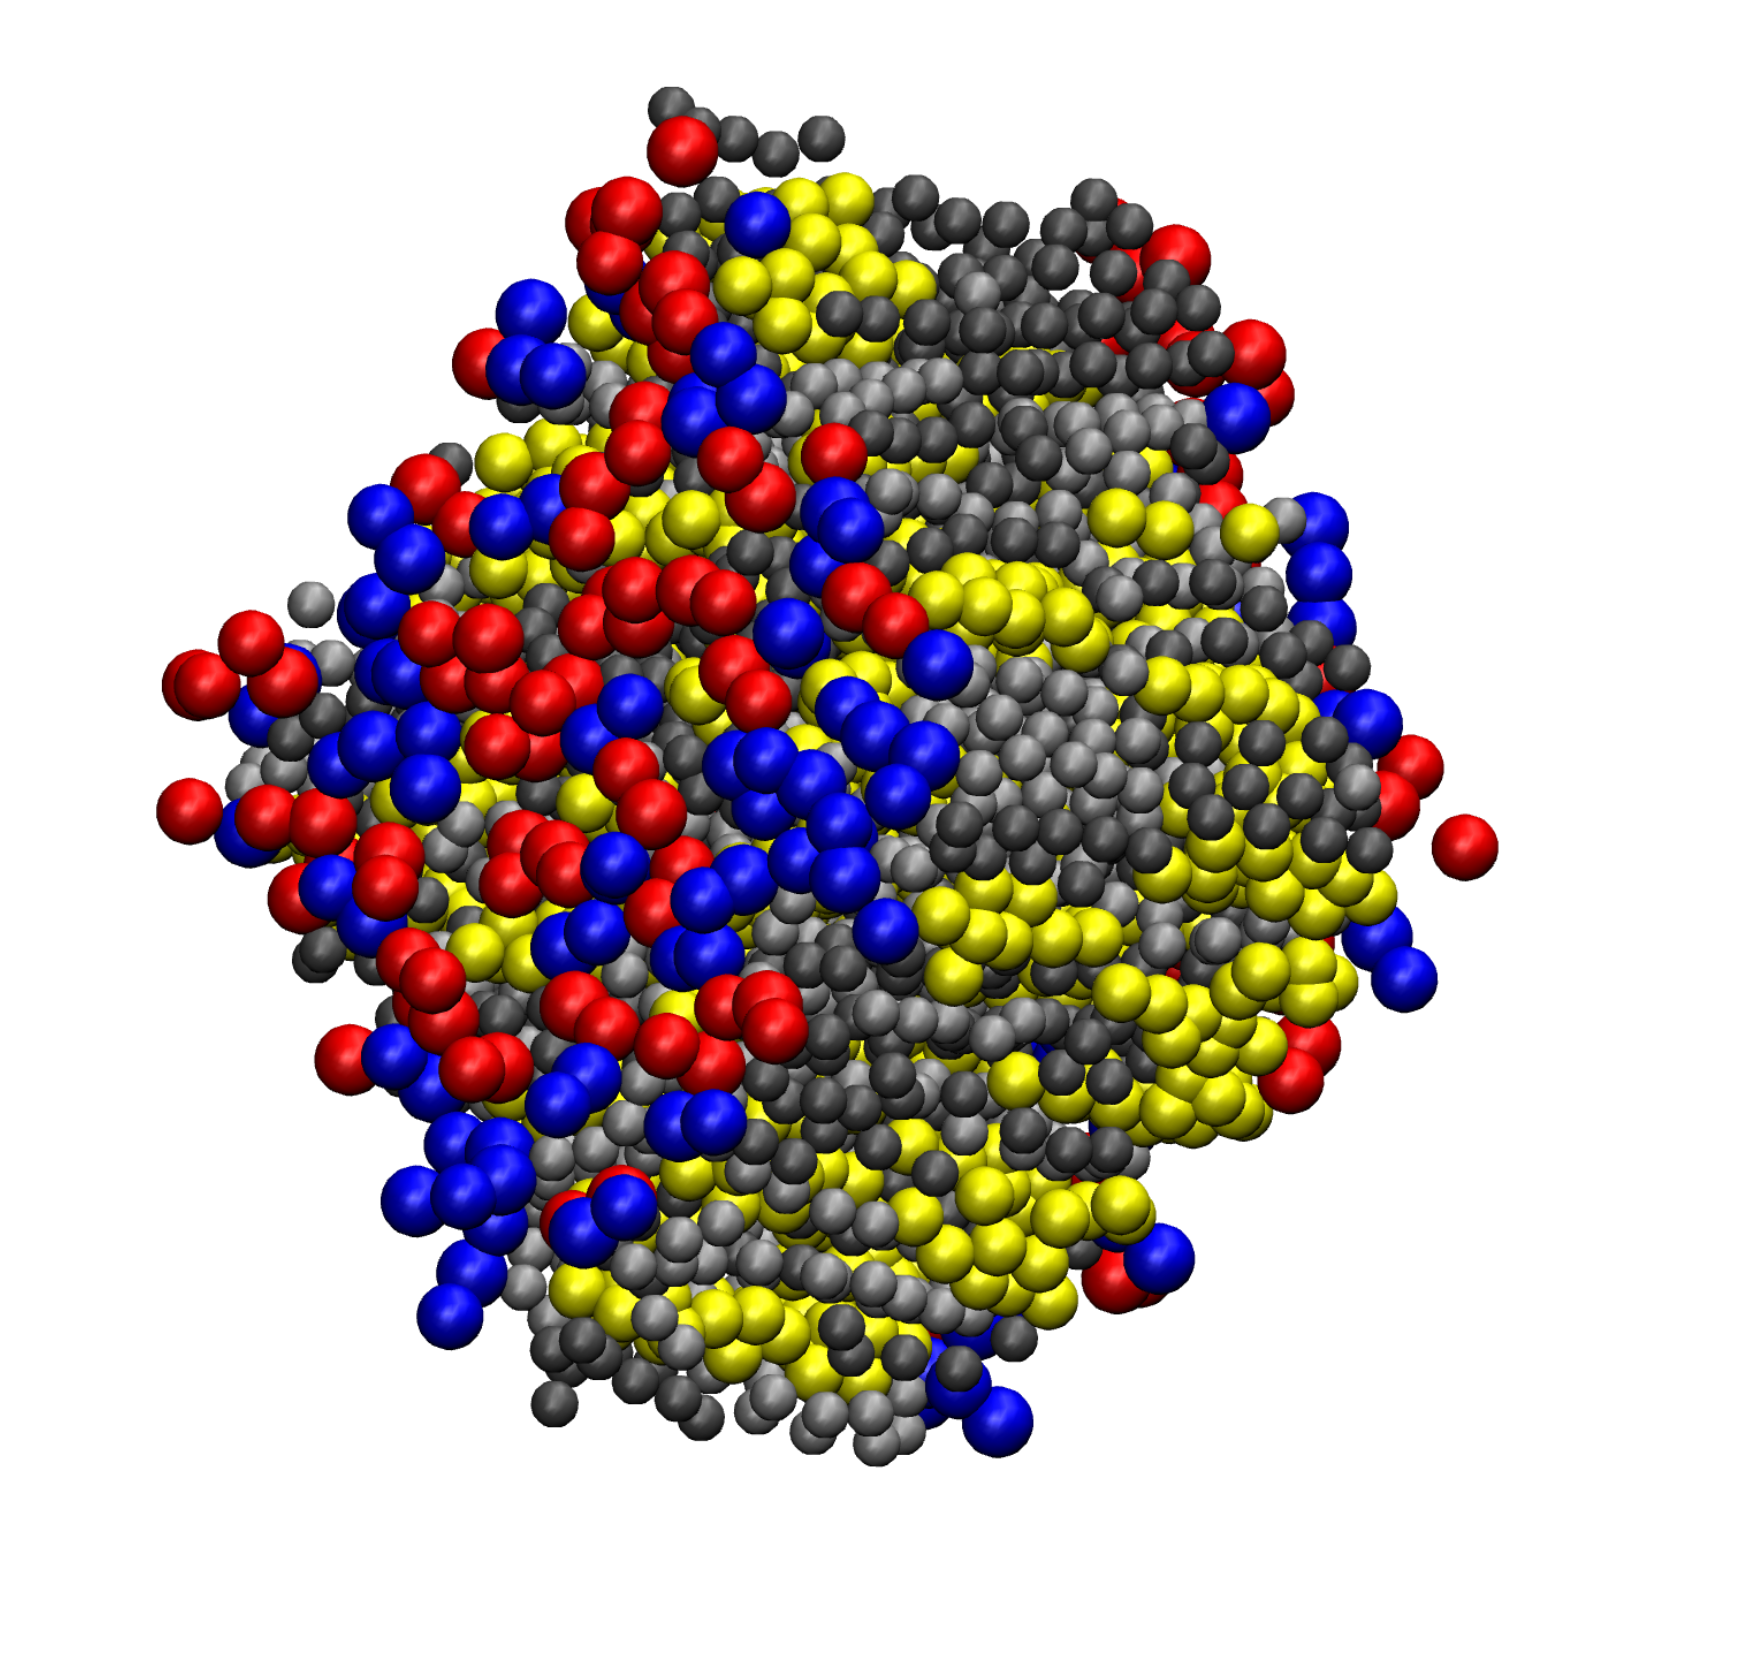
\includegraphics[width=\textwidth]{imagens/img7.jpg}
        \caption{Frame $t_5$}
    \end{subfigure}
    \hfill
    \begin{subfigure}[b]{0.24\textwidth}
        \centering
        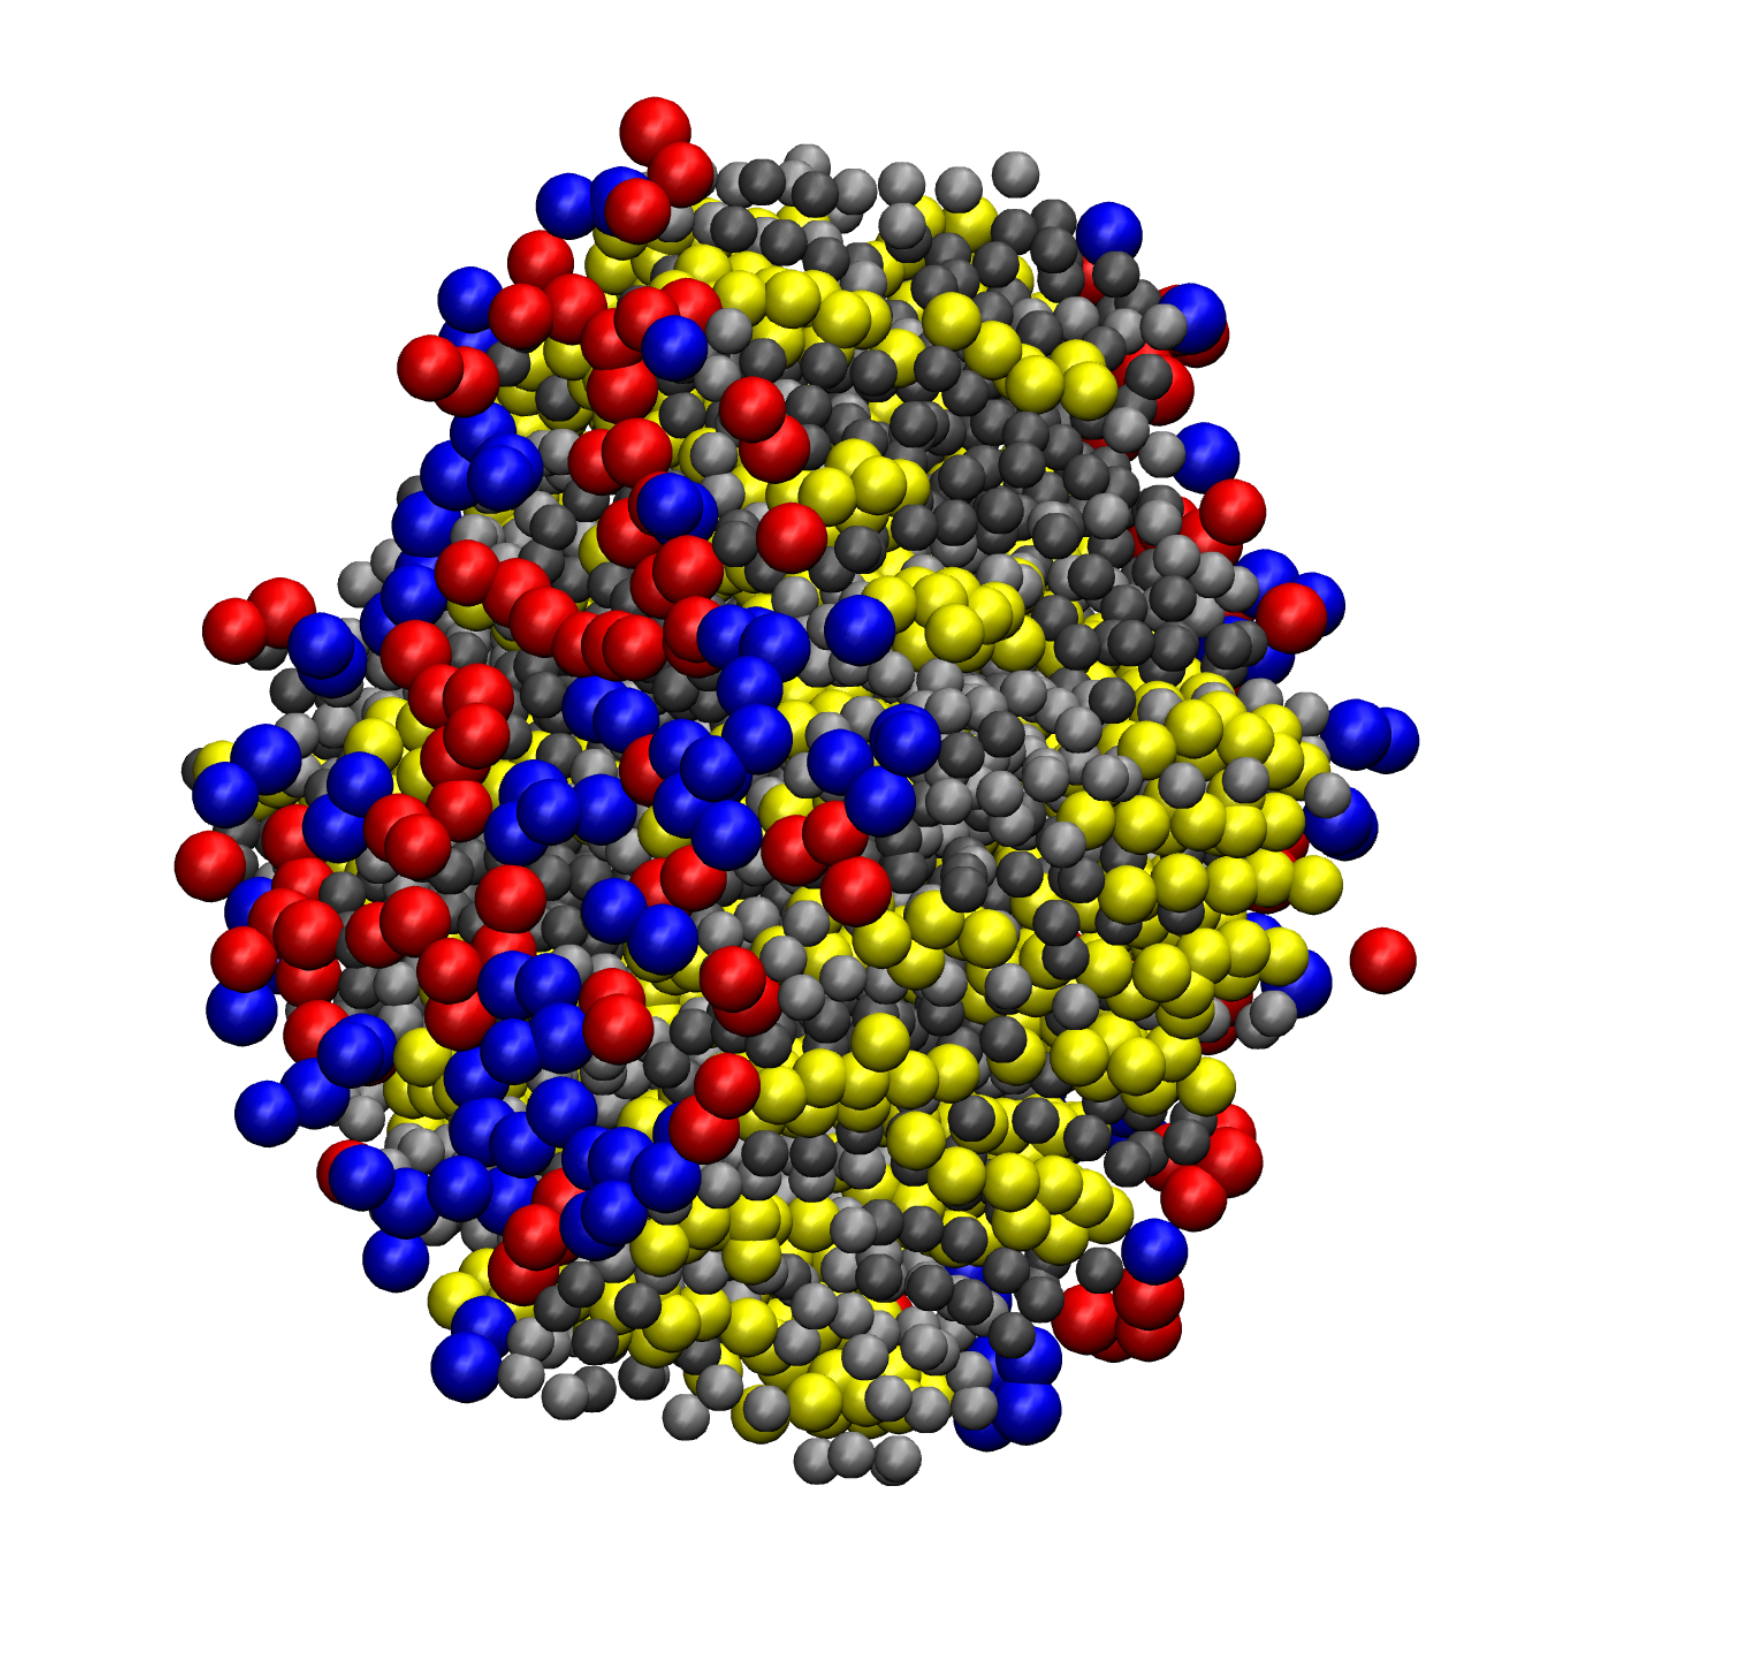
\includegraphics[width=\textwidth]{imagens/img8.jpg}
        \caption{Frame $t_6$}
    \end{subfigure}
    \hfill
    \begin{subfigure}[b]{0.24\textwidth}
        \centering
        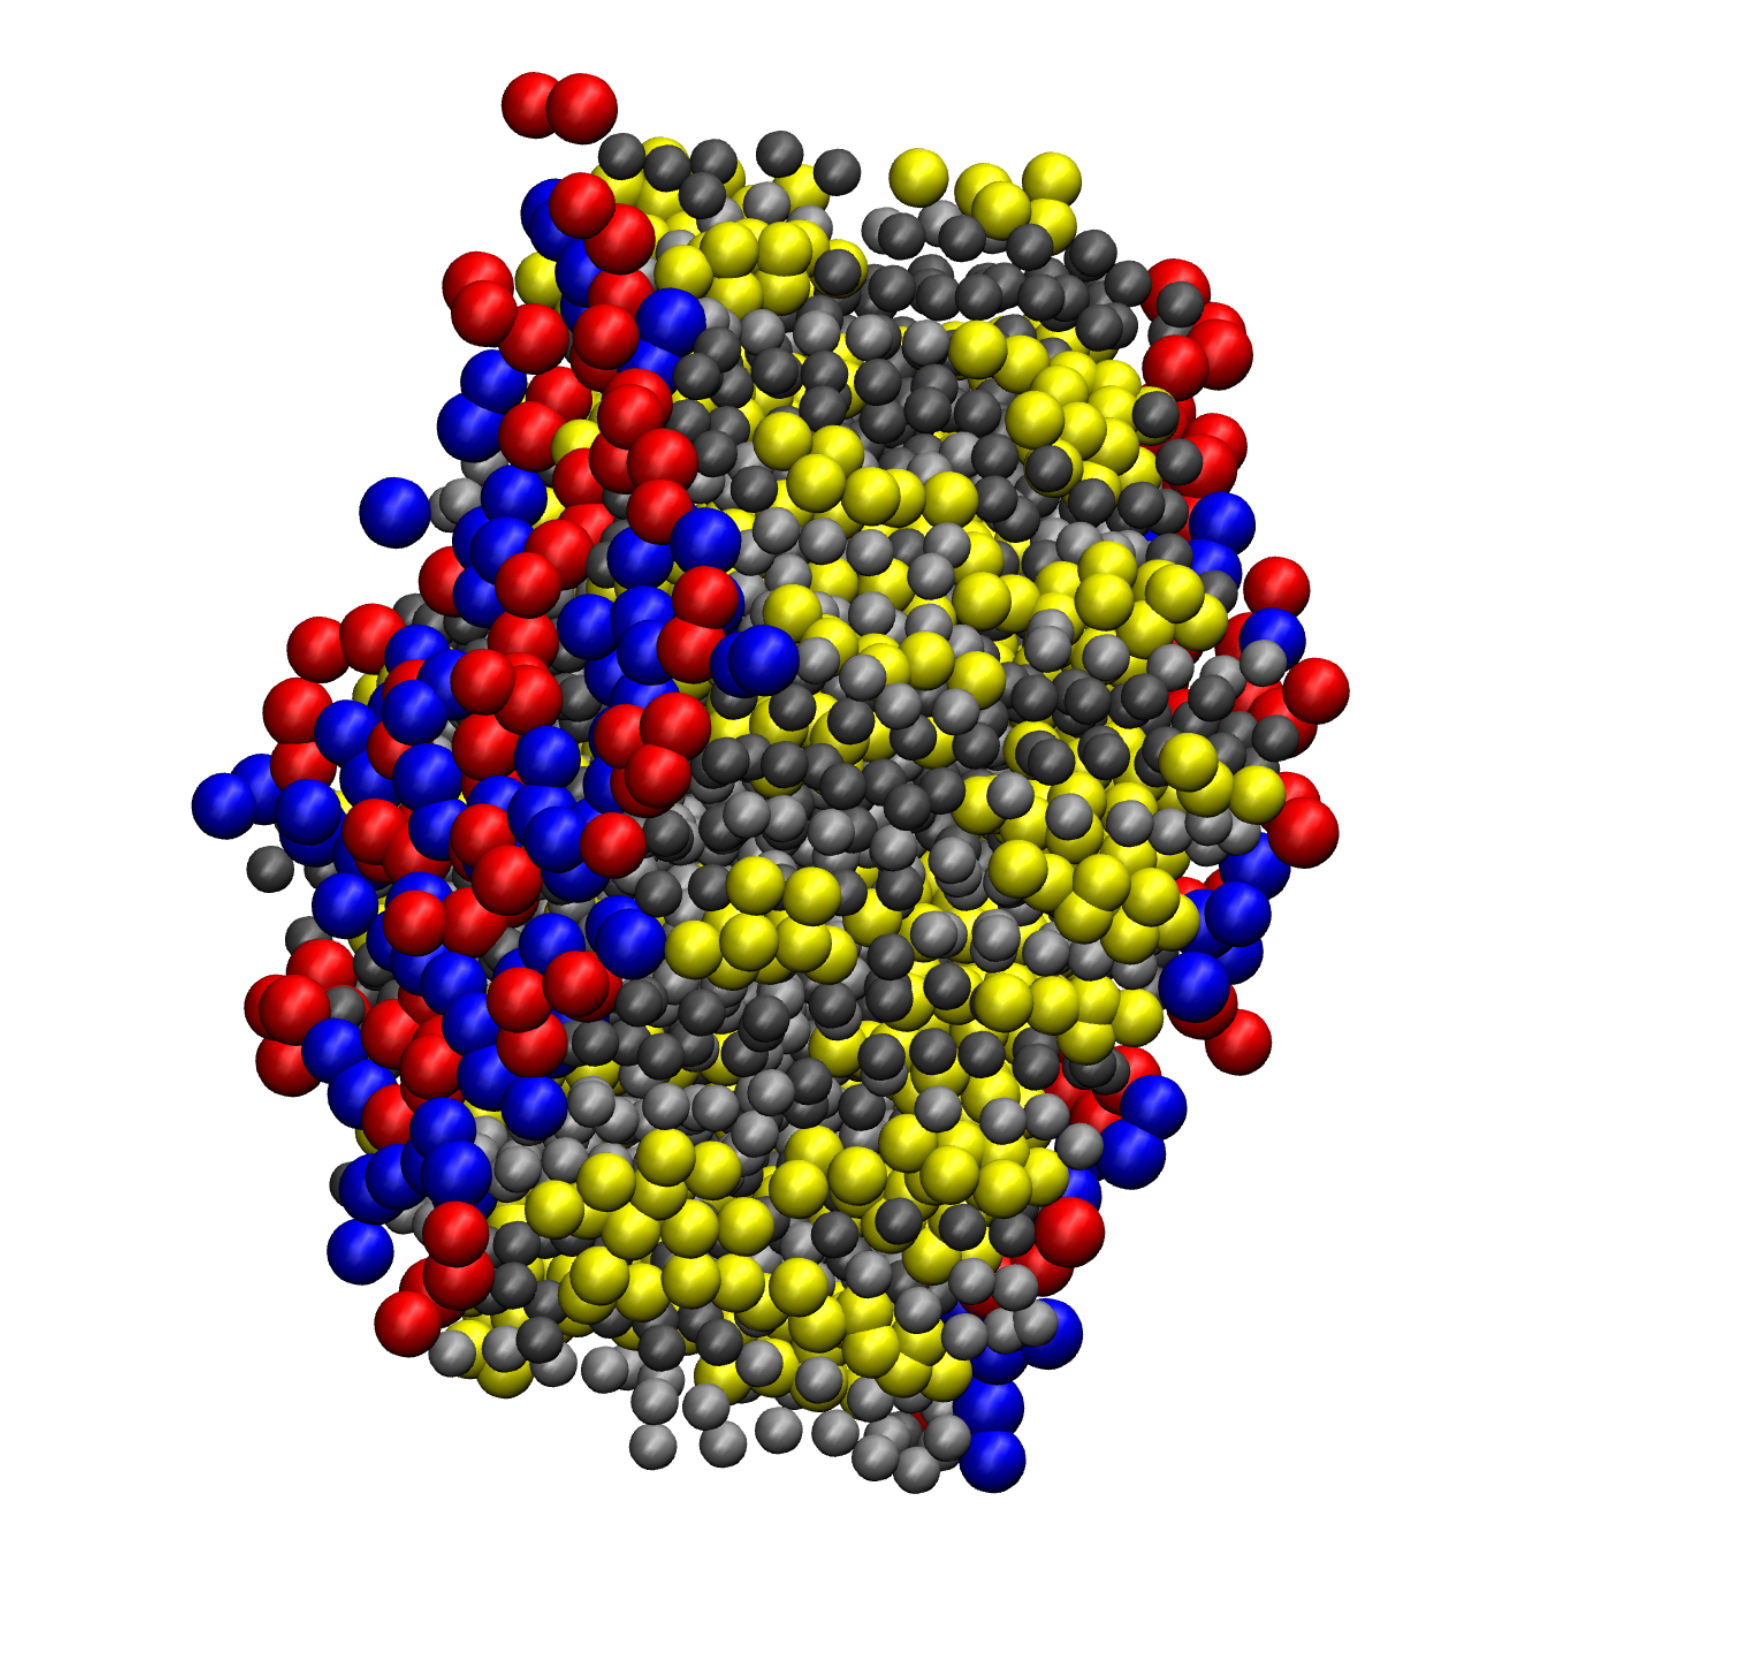
\includegraphics[width=\textwidth]{imagens/img9.jpg}
        \caption{Frame $t_7$}
    \end{subfigure}

    \caption{Mosaico do sistema DPPC/DSPC/Colesterol (40\% mol) a 333 K. Em (a), observa-se a vista lateral evidenciando o empacotamento das caudas. De (b) a (h), a evolução temporal confirma que a mistura se mantém estável, sem separação macroscópica de fases, com o colesterol (amarelo) dinamicamente intercalado e homogeneamente distribuído pelo núcleo hidrofóbico, sustentando a fase líquida-ordenada ($L_o$). (Fonte: Autoria própria).}
    \label{fig:mosaico_dinamico}
\end{figure}

\subsubsection*{Perfil de Solvatação e Coordenação Iônica}

Para observar a difusão dos eletrólitos na interface polar, optou-se por uma renderização com escala atômica ajustada. Ao atenuar os raios de van der Waals da malha hídrica e ampliar os de sódio e cloreto, o mapeamento dos beads torna-se evidente. \ref{fig:vmd_solvatacao}).

\begin{figure}[H]
    \centering
    % ================= TOPO: PANORÂMICA (Vista Lateral) =================
    \begin{subfigure}[b]{0.95\textwidth}
        \centering
        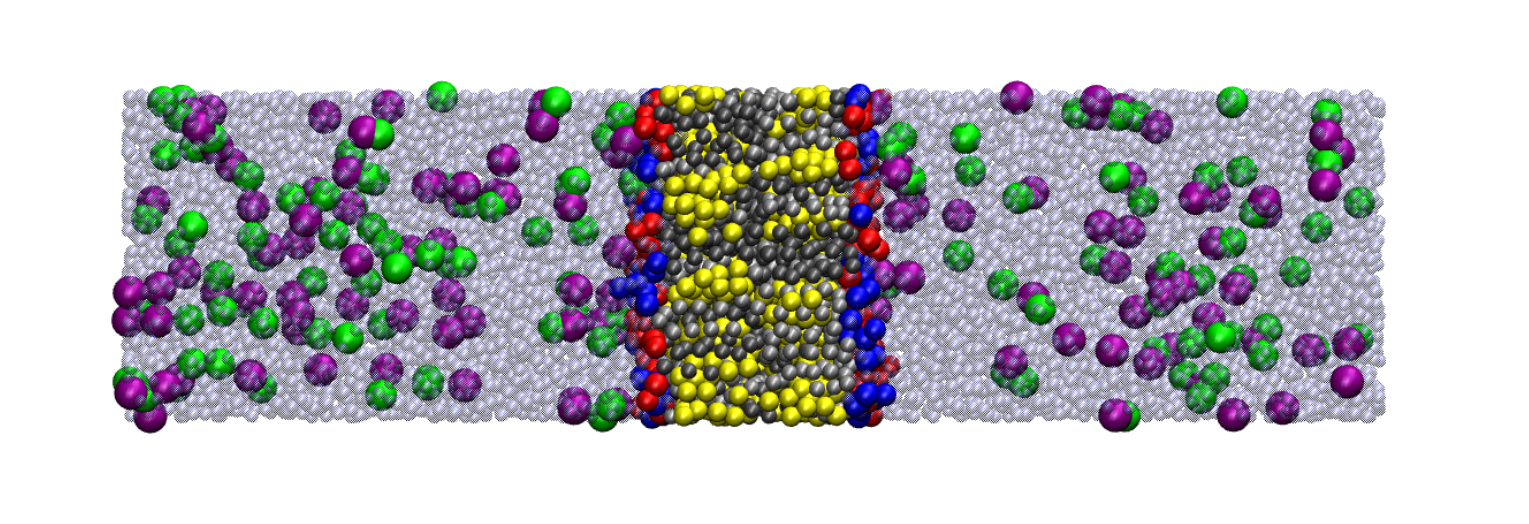
\includegraphics[width=\textwidth]{imagens/img_panoramica_140505.png} 
        \caption{Corte transversal evidenciando a completa solvatação da bicamada}
    \end{subfigure}

    \vspace{0.6cm} 

    % ================= BASE: 3 PERSPECTIVAS LADO A LADO =================
    \begin{subfigure}[b]{0.31\textwidth}
        \centering
        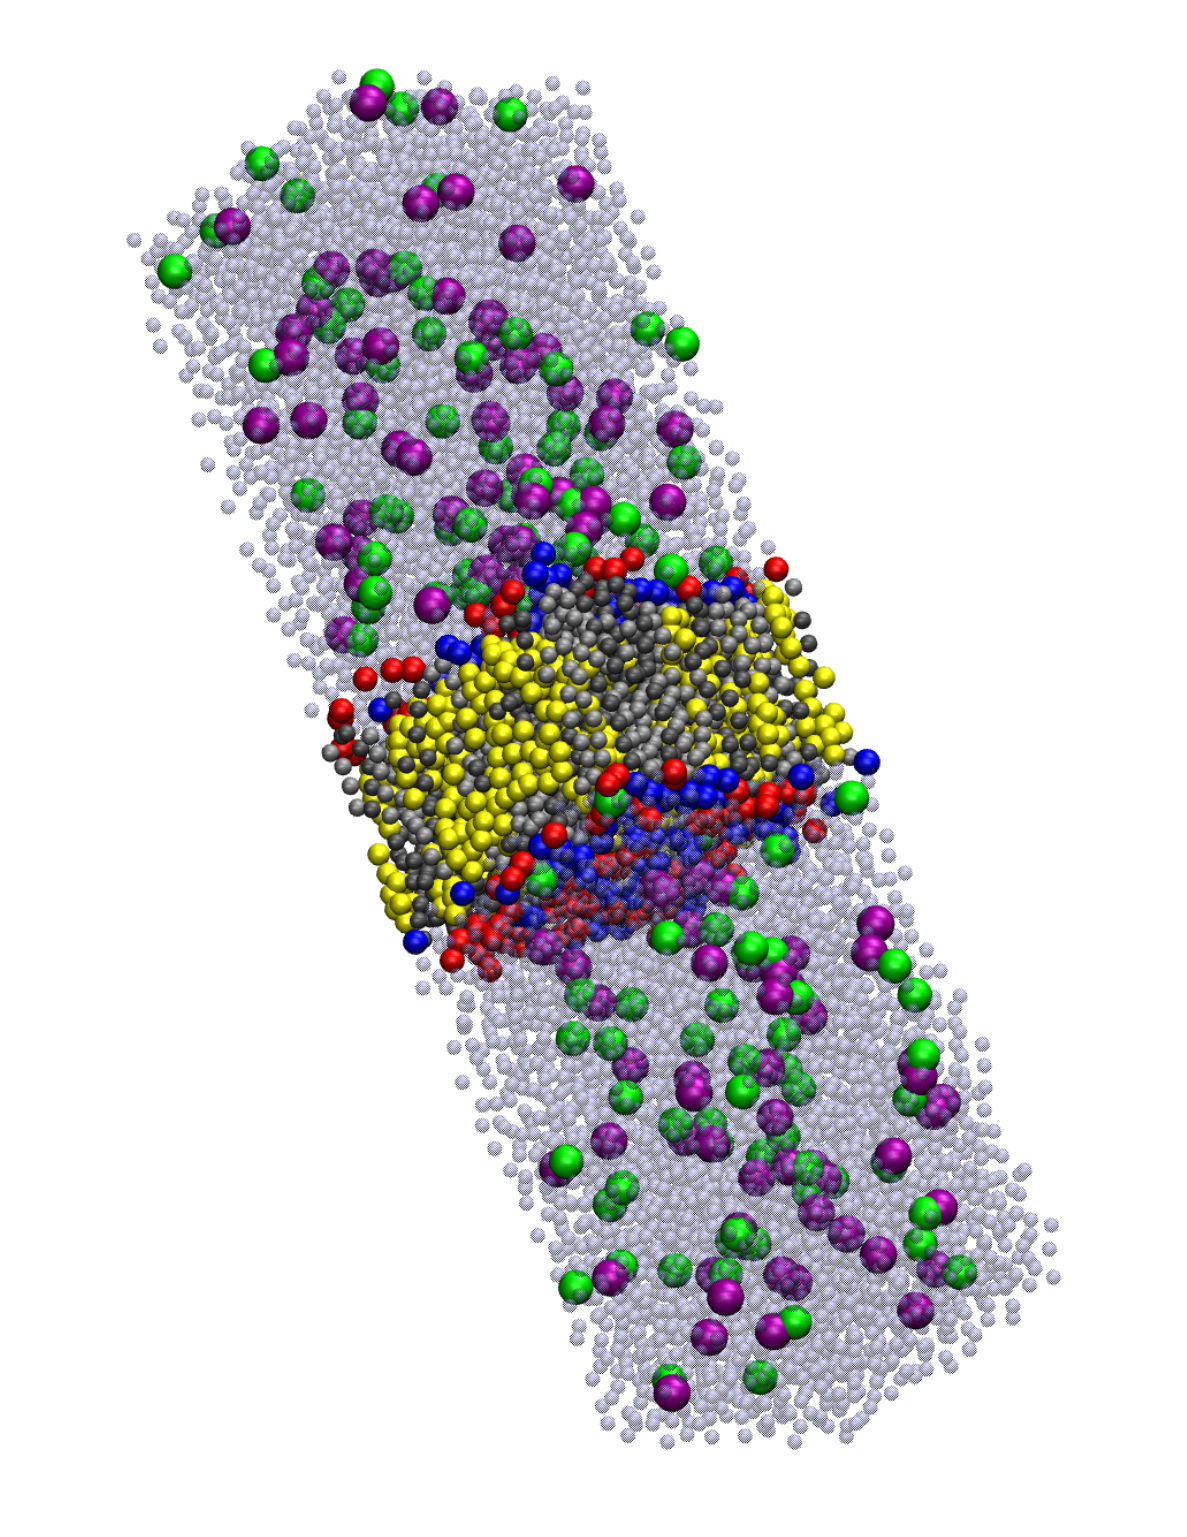
\includegraphics[width=\textwidth]{imagens/img_persp_135957.png} 
        \caption{Vista isométrica A}
    \end{subfigure}
    \hfill
    \begin{subfigure}[b]{0.31\textwidth}
        \centering
        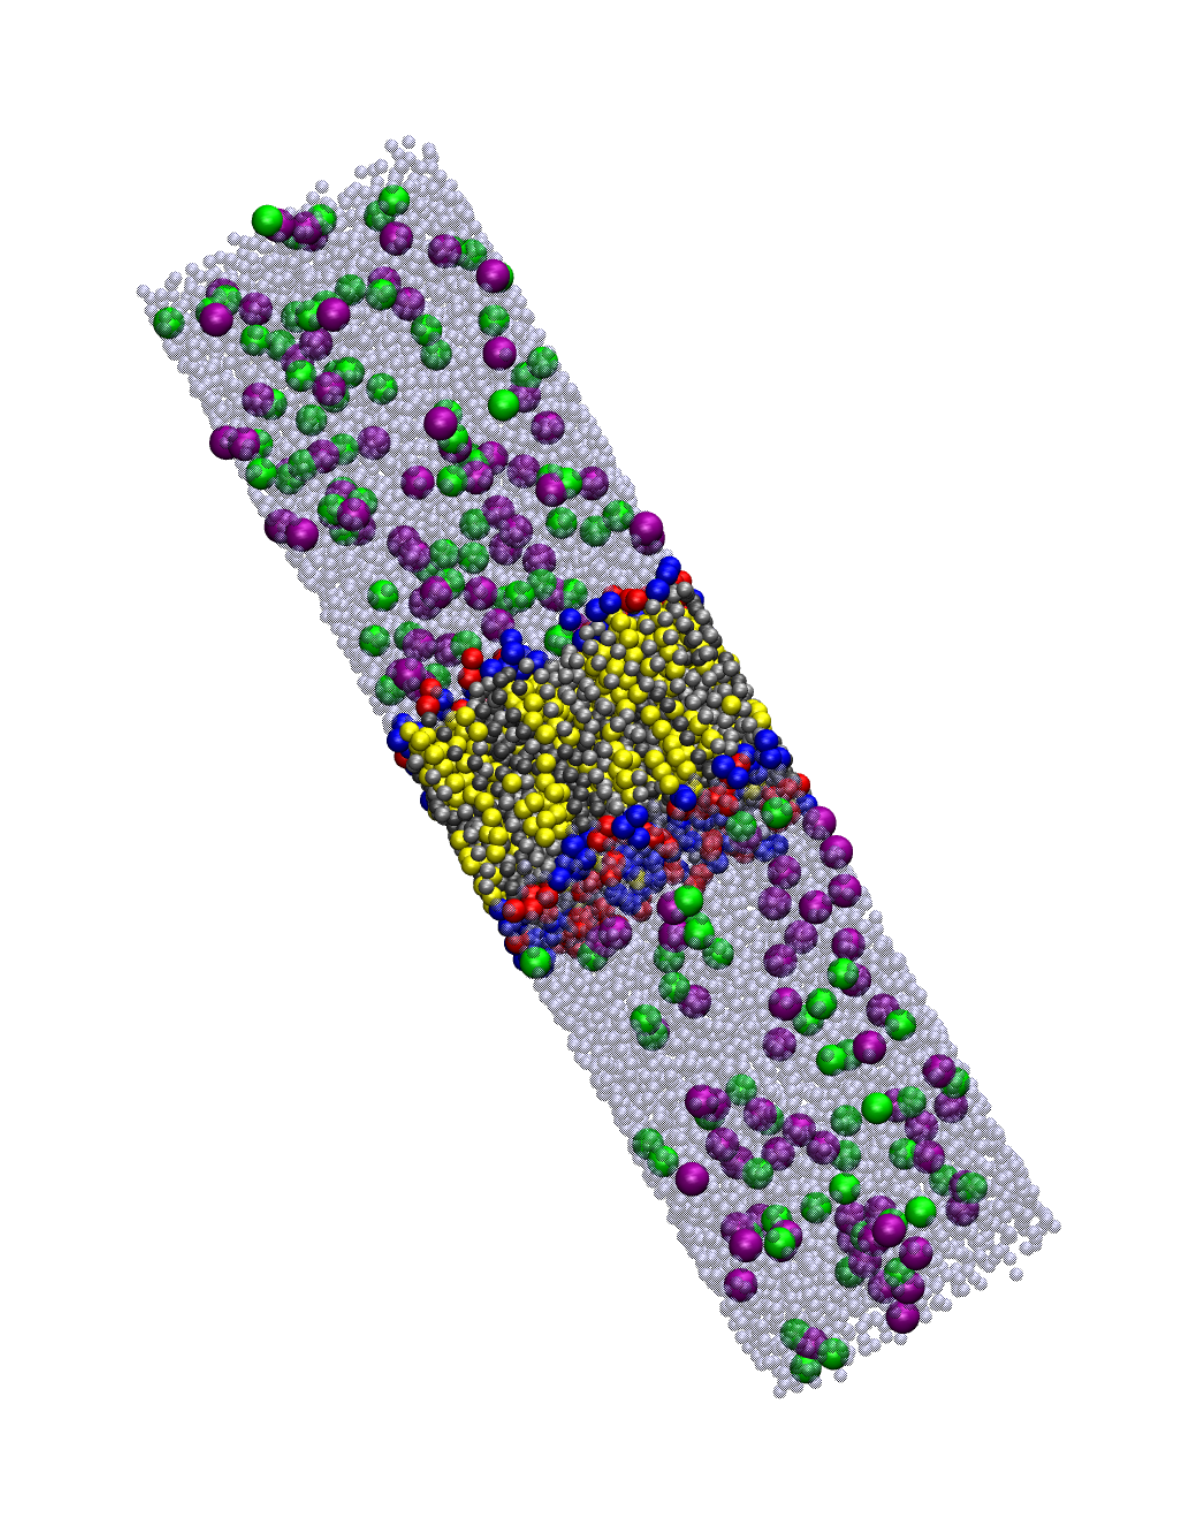
\includegraphics[width=\textwidth]{imagens/img_persp_140217.png} 
        \caption{Vista isométrica B}
    \end{subfigure}
    \hfill
    \begin{subfigure}[b]{0.31\textwidth}
        \centering
        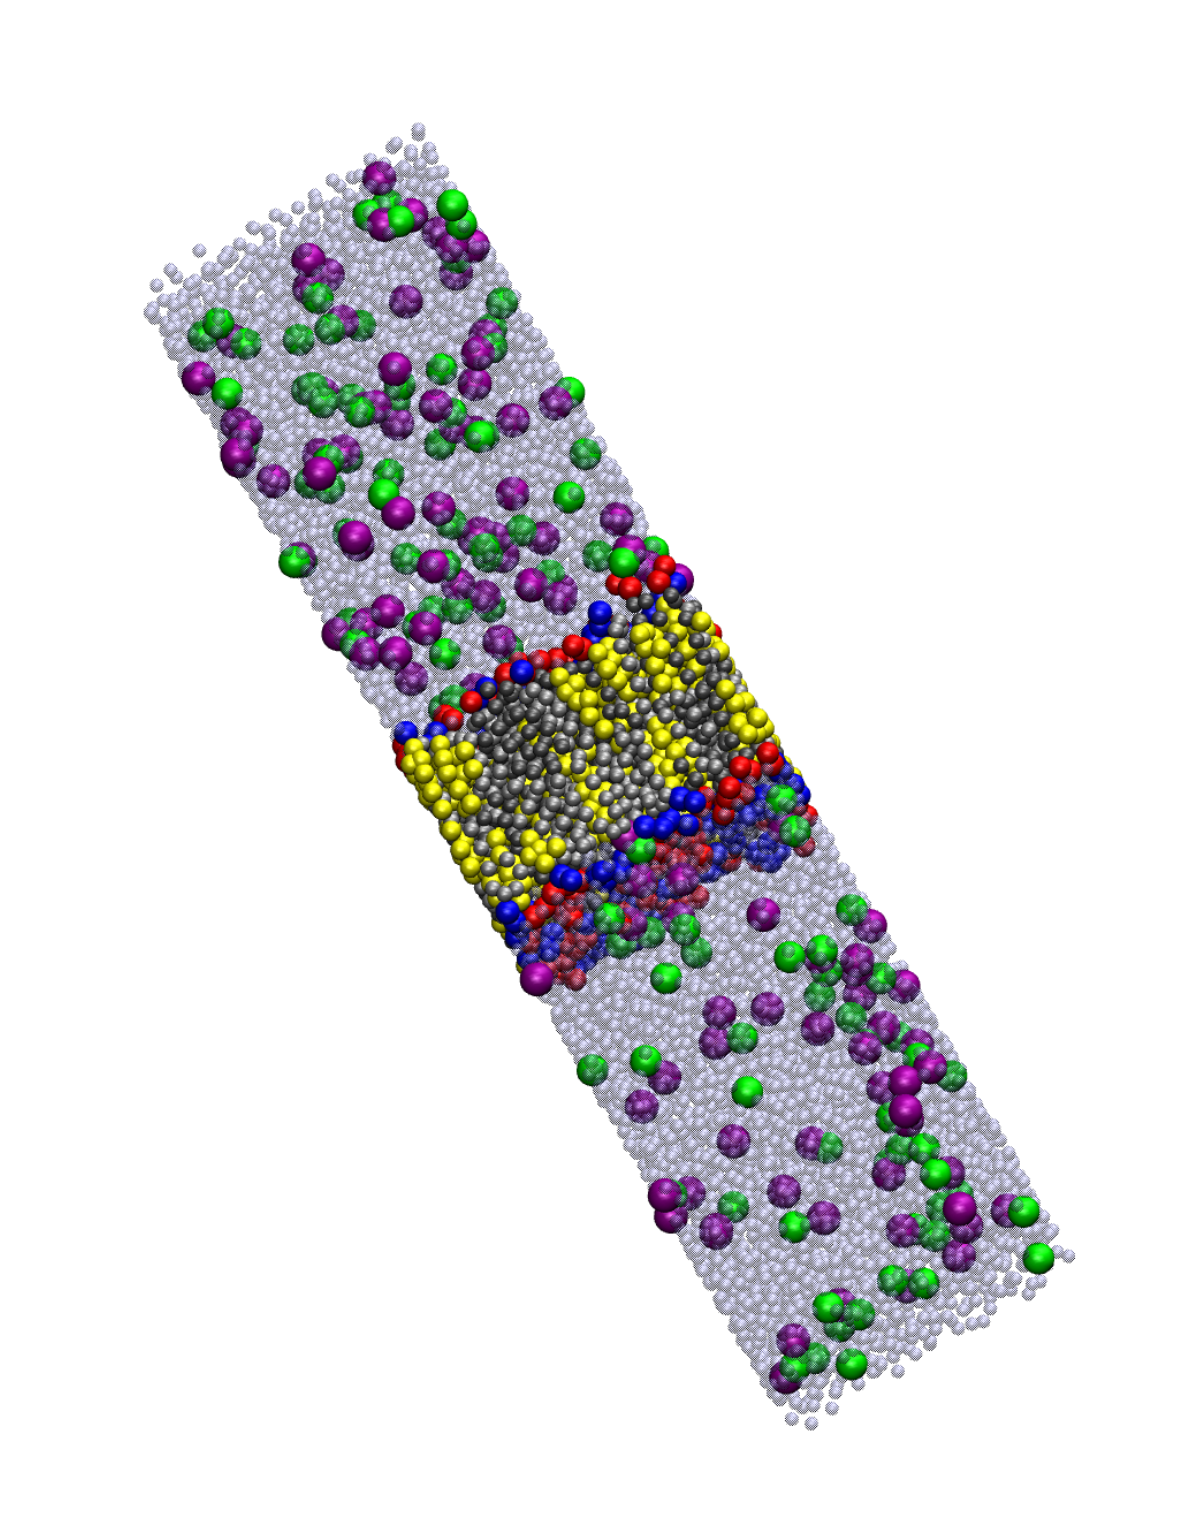
\includegraphics[width=\textwidth]{imagens/img_persp_140322.png} 
        \caption{Vista isométrica C}
    \end{subfigure}

    \caption{Solvatação e distribuição iônica do sistema DPPC/DSPC/Colesterol em meio salino a 333 K. Utilizou-se uma escala atômica modificada: a malha de água (esferas azuis translúcidas) apresenta raio reduzido, enquanto os íons de Na$^+$ (verde) e Cl$^-$ (roxo) encontram-se ampliados, destacando a sua distribuição volumétrica na fase aquosa e a ausência de permeação no núcleo hidrofóbico denso ($L_o$). (Fonte: Autoria própria).}
    \label{fig:vmd_solvatacao}
\end{figure}

\subsubsection*{Mismatch Hidrofóbico e Acomodação Interfacial}

A resposta topológica da membrana à disparidade do comprimento das cadeias acílicas (\textit{hydrophobic mismatch}) encontra-se ilustrada na Figura \ref{fig:mosaico_mismatch}. O comparativo visual espelha o ganho de espessura transversal e as alterações na distribuição geométrica da solvatação discutidas nas análises termodinâmicas anteriores.

\begin{figure}[H]
    \centering
    % ================= LINHA 1: Vistas Laterais =================
    \begin{subfigure}[b]{0.26\textwidth}
        \centering
        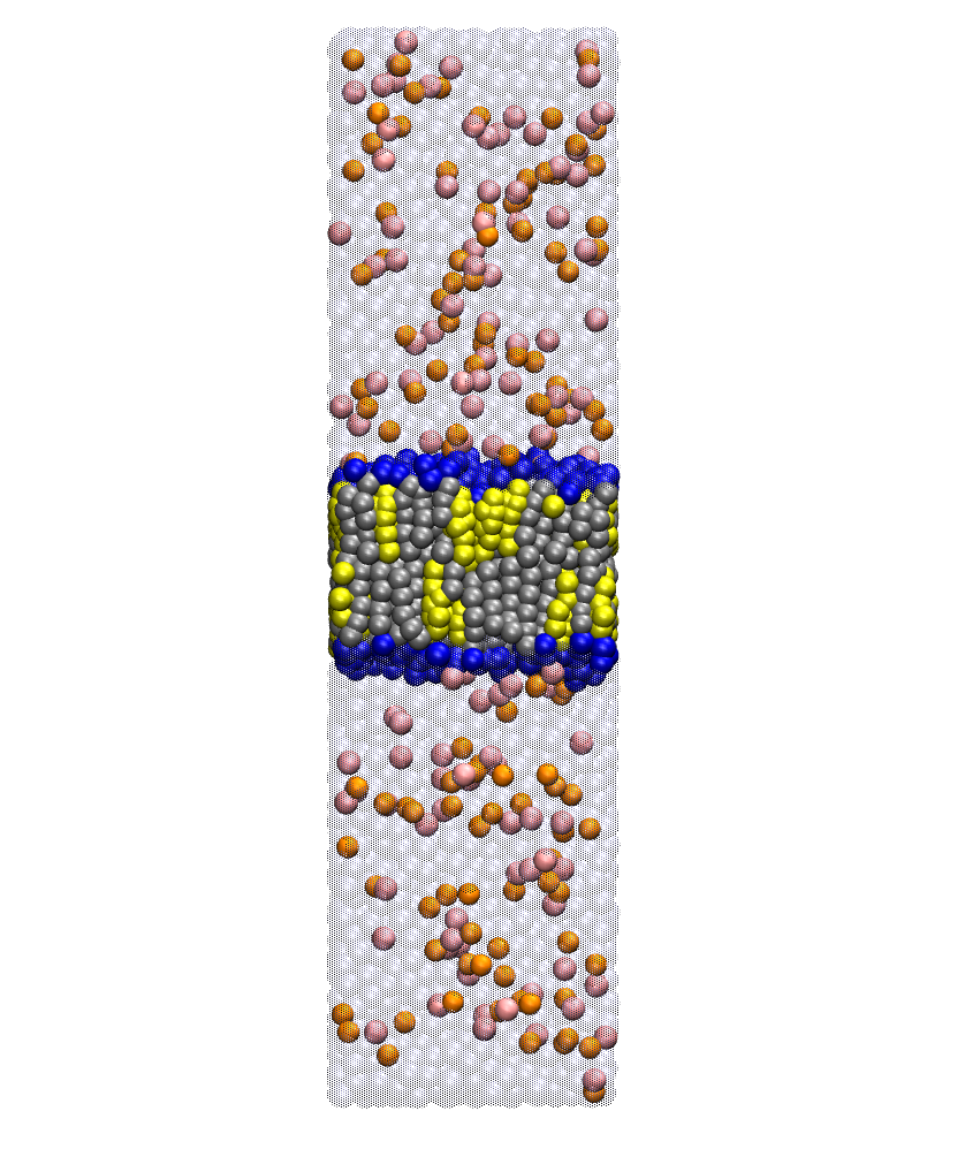
\includegraphics[width=\textwidth]{imagens/dppc_lat.png}
        \caption{DPPC (C16) - Vista Lateral}
    \end{subfigure}
    \hspace{1.5cm} 
    \begin{subfigure}[b]{0.26\textwidth}
        \centering
        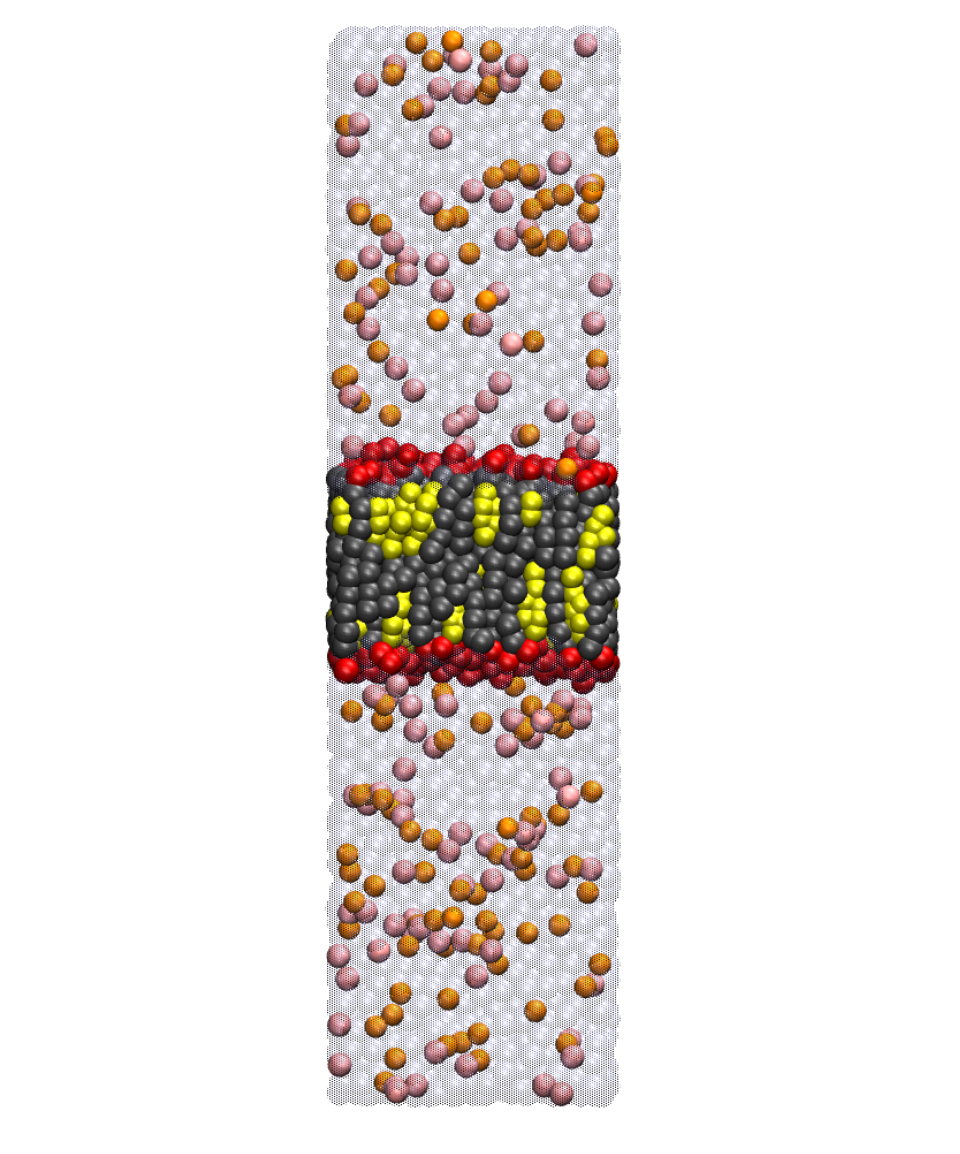
\includegraphics[width=\textwidth]{imagens/dspc_lat.png}
        \caption{DSPC (C18) - Vista Lateral}
    \end{subfigure}

    \vspace{0.5cm} 

    % ================= LINHA 2: Vistas Isométricas =================
    \begin{subfigure}[b]{0.26\textwidth}
        \centering
        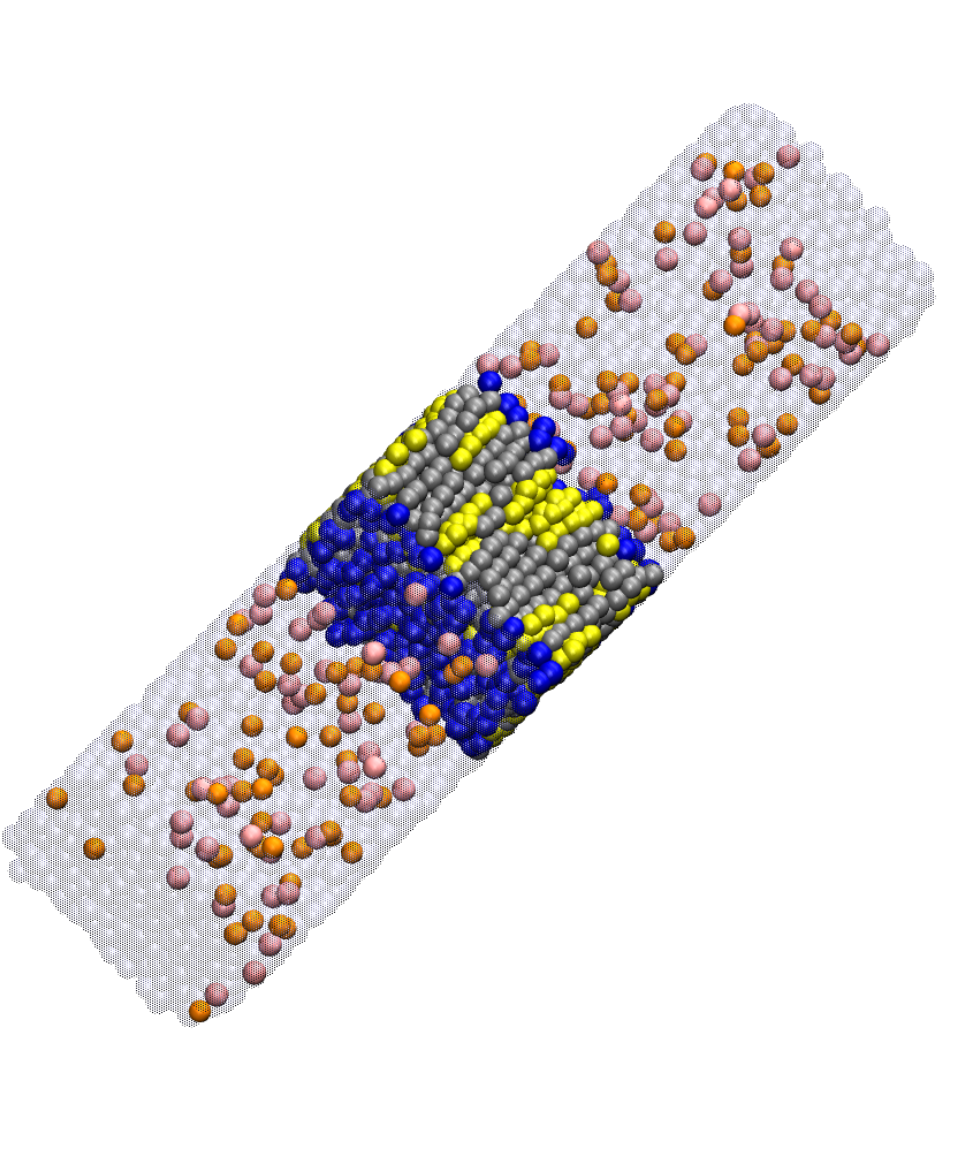
\includegraphics[width=\textwidth]{imagens/dppc_iso.png}
        \caption{DPPC (C16) - Perspectiva}
    \end{subfigure}
    \hspace{1.5cm} 
    \begin{subfigure}[b]{0.26\textwidth}
        \centering
        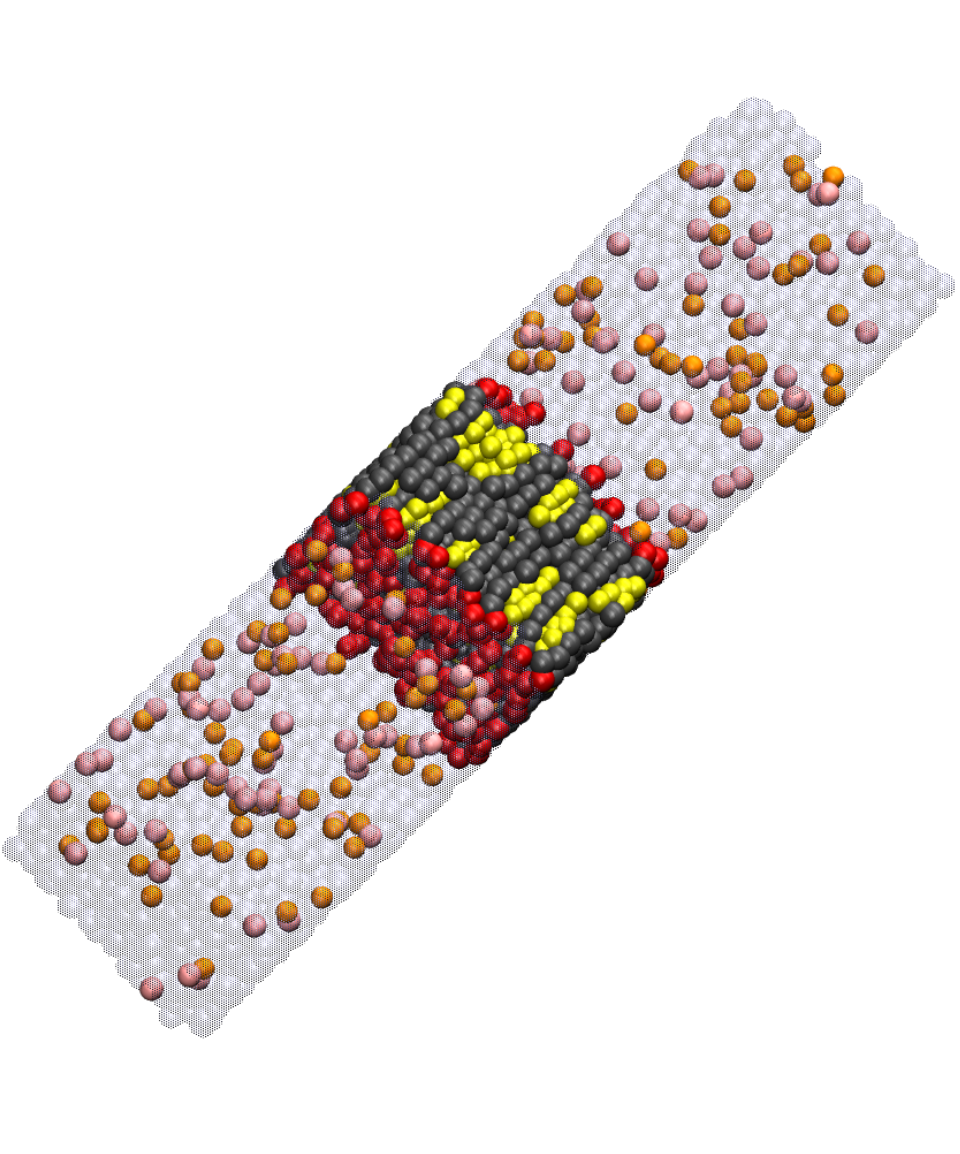
\includegraphics[width=\textwidth]{imagens/dspc_iso.png}
        \caption{DSPC (C18) - Perspectiva}
    \end{subfigure}

    \caption{Comparativo visual do efeito do comprimento da cadeia acílica (\textit{mismatch} hidrofóbico) na estrutura da bicamada a 310 K. À esquerda, o sistema composto por DPPC (16 carbonos) apresenta um núcleo hidrofóbico mais estreito. À direita, o sistema composto por DSPC (18 carbonos) possui maior espessura de membrana. (Fonte: Autoria própria).}
    \label{fig:mosaico_mismatch}
\end{figure}






% =====================================================================
% SECÇÃO 4.5 - PERSPECTIVAS FUTURAS E METODOLOGIA
% =====================================================================


% =====================================================================
% SECÇÃO 4.5 - PERSPECTIVAS FUTURAS E SEEDING
% =====================================================================

\subsection{Perspectivas Futuras: Aprimoramentos Paramétricos e Nucleação Assistida (\textit{Seeding})}

Conforme demonstrado nas análises termodinâmicas, o aprisionamento do DSPC em um estado metaestável não decorre de artefatos de simulação, mas de uma autêntica barreira entálpica de dessolvatação intrínseca ao modelo \textit{coarse-grained}. A inércia estrutural observada nos protocolos de resfriamento contínuo (\textit{simulated annealing}) corrobora estudos recentes do lipidoma Martini 3, que atestam uma histerese significativa neste tipo de amostragem térmica \cite{pedersen2024}. 

Para investigações futuras que demandem a determinação exata e livre de histerese da temperatura de transição ($T_m$), sugere-se a aplicação metodológica da nucleação assistida (\textit{seeding}). Com base nas configurações validadas para este campo de força \cite{pedersen2024}, o refinamento topológico e termodinâmico no GROMACS deve seguir as seguintes diretrizes:

A montagem de membranas heterogêneas contendo ilhas sólidas (fase gel) inseridas em matrizes líquidas encontra limitações no clássico \textit{script insane}. Recomenda-se a ferramenta \textit{Coarse-Grained System Builder} (COBY), projetada especificamente para viabilizar a inserção de um \textit{patch} lamelar estruturado ($L_\beta$) no núcleo da membrana fluida ($L_\alpha$) sem provocar sobreposições destrutivas.

A estabilização do sistema exige banhos térmicos independentes na mesma topologia, devido a uma limitação arquitetural do GROMACS, o barostato estocástico \textit{c-rescale} não suporta múltiplos grupos de acoplamento térmico (\texttt{tc-grps}). Portanto, é obrigatório o uso temporário do barostato Berendsen ($\tau_p = 4,0$ ps) unicamente durante o relaxamento da interface de coexistência. Com a interface estabilizada, o controle de temperatura é unificado e o sistema deve obrigatoriamente retornar ao barostato \textit{c-rescale} semi-isotrópico para a execução das trajetórias de varredura térmica que ditarão a $T_m$ exata.\cite{pedersen2024}. Mudanças no protocolo utilizado podem aprimorar os resultados simulados.

A adoção de uma reparametrização no tamanho dos beads de acordo com os centros de massa dos agrupamentos atômicos pode contribuir para uma melhor resolução do campo de força Martini 3, garantindo alta exatidão física.
